\documentclass[10pt,a4paper]{article}
\usepackage{float}
\usepackage{verbatim}
\usepackage[utf8]{inputenc}
\usepackage[italian]{babel}
\usepackage{amsmath}
\usepackage{amsbsy}
\usepackage{amsfonts}
\usepackage{amssymb}
\usepackage{graphicx}
\usepackage[left=2cm,right=2cm,top=2cm,bottom=2cm]{geometry}
\usepackage{xcolor}
\usepackage{amsthm}
\usepackage{mhchem}
\usepackage[hypertexnames=false]{hyperref}
\usepackage{nameref}
\usepackage{multicol}

\hypersetup{
    pdftitle={title},
    pdfsubject={subject},
    pdfauthor={author},
}

% comandi richiamati
\newcommand{\numberset}{\mathbb}
\newcommand{\Q}{\numberset{Q}}
\newcommand{\I}{\numberset{I}}
\renewcommand\thepart{\arabic{part}}
\renewcommand\thesection{\alph{section}}
\renewcommand\thesubsection{\thepart.\thesection.\arabic{subsection}}
\newcommand{\parallelsum}{\mathbin{\|}}

\author{Edoardo Gabrielli}
\title{Checklist per l'esame di Fisica 3}

\begin{document}

\maketitle
Ispirato alla Checklist creata in precedenza da \ldots ha voluto scrivere e condividere anche la mia, sperando che sia utile e che la facciate vostra negli anni a venire, infati tutto il codice sorgente sarà reperibile sulla pagina Git \ldots per chiunque voglia scaricare e prendere ciò che c'è di buono. Buona lettura e buono studio.
\clearpage

\begin{multicols}{2}
	\tableofcontents
\end{multicols}

\listoffigures
\clearpage


\pagenumbering{arabic}
\part{Prerequisiti}
\section{Domande a}
\subsection[ $\beta$, $\gamma$]{Definire le quantità $\beta$ e $\gamma$ per le trasformazioni di Lorentz.} 
Presi due sistemi di riferimento inerziali $O$ ed $O'$ si ha che $\beta$ è la velocità del sistema $O'$ rispetto ad $O$ (in unità di c) mentre:
\[
	\gamma = \frac{1}{\sqrt{1-\beta^2}}
.\] 

\subsection[ Prodotto scalare nella metrica di Minkowsky]{Definire il prodotto scalare di due 4-vettori.} 
Presi $x^{\mu} = (x^0,\boldsymbol{x})$ e $y^{\mu} = ( y^0, \boldsymbol{y})$ si definisce il loro prodotto come $x^{\mu}y_{\nu}$ come:
\[
x^{\mu}y_{\nu} = x^{0}y^{0}-\boldsymbol{x} \cdot \boldsymbol{y} 
.\] 
\subsection[ Modulo di un quadrivettore]{Definire il modulo di un 4-vettore.}
Se $x^{\mu}$ è un 4-vettore il suo modulo è definito secondo la metrica:
\[
|x|^2 = x^{\mu}x_{\mu}
.\] 
Dato che il tensore metrico non è definito positivo il modulo di un 4-vettore può esser positivo, negativo o nullo. 
\subsection[ Trasformazioni di Lorentz]{Scrivere le trasformazioni di Lorentz per il boost lungo un asse (asse x).}
Per un boost lungo l'asse x si ha:
\[
\begin{cases}
	ct' = \gamma ( ct - \beta x) \\	
	x' = \gamma (x - \beta ct ) \\
	y' = y \\
	z' = z
\end{cases}
\]
o in forma matriciale:

\[
\left( \begin{array}{c} ct' \\ x' \\ y' \\ z' \end{array} \right)
= 
\begin{pmatrix}
	\gamma  & -\gamma \beta  & 0 & 0\\
	- \gamma \beta & \gamma & 0 & 0\\
	0 & 0 & 1 & \\
	0 & 0 & 0 & 1 \\
\end{pmatrix}
\left( \begin{array}{c} ct \\ x \\ y \\ z  \end{array} \right)
\] 

\subsection[ Operatori differenziali 4-dimensionali]{Definire le derivate in 4-dimensioni, la quadridivergenza, il differenziale di uno scalare di Lorentz, l’operatore di D’Alembert.}
Si definisce gli operatori $\partial^{\mu}$ e $\partial_{\mu}$ come:
\[
	\partial^{\mu} = \left( \frac{1}{c} \frac{\partial}{\partial t} , - \nabla  \right) ,\quad
	\partial_{\mu} = \left(\frac{1}{c} \frac{\partial}{\partial t} ,  \nabla  \right)
.\] 
Preso un generico campo tensoriale, la sua 4-divergenza (rispetto a qualche indice) è la contrazione tra l'operatore $\partial^{\mu}$ e l'indice stesso (se ques'ultimo è covariante) oppure tra l'operatore $\partial_{mu}$ e l'indice stesso (se quest'ultimo è controvariante). Ad esempio preso il campo vettoriale $v^{\mu} \equiv \left(v^{0}, \boldsymbol{v}\right)$ la sua 4-divergenza sarà:
\[
\partial_{\mu}v^{\mu} = \frac{1}{c} \frac{\partial v^{0}}{\partial t} + \nabla \boldsymbol{v} 
.\]
Se invece $\phi$ è un invariante di Lorentz il suo differenziale è:
 \[
	 d\phi = dx^{\mu}\partial_{\mu}\phi = \frac{\partial\phi}{\partial t}dt + \left(d \boldsymbol{x}\cdot \nabla \right)\phi  
.\]
L'operatore di D'Alembert invece è: 
\[
	\Box = \partial_{\mu}\partial^{\mu} = \frac{1}{c^{2}}\frac{\partial^{2}}{\partial t^{2}}    
.\] 
\subsection[ Tempo proprio]{Definire il tempo proprio e dare la relazione (differenzale) fra tempo proprio e tempo nel sistema in cui si osserva il moto.}
Si sa che l'intervallo $ds^{2}$ è uno scalare di Lorentz, inoltre per un sistema solidale (o tangente) si ha $dx^{\mu} = \left( cd\tau, 0 \right)$ con $d\tau$ il tempo proprio infinitesimo. Si ha quindi: 
\[
		c^{2}d\tau^{2} = c^{2}d\tau^{2} - |dx|^{2} = c^{2}dt^{2} -|\boldsymbol{v}|^{2}dt^{2} \implies d\tau = \frac{dt}{\gamma} 
.\] 
\subsection[ Invariante di Lorentz]{Dare la definizione di invariante di Lorentz.} 
Un invariante di Lorentz è una grandezza che viene lasciata invariata dalle trasformazioni di Lorentz: è uguale in tutti i sistemi di riferimento inerziali.
\subsection[ 4-velocità e 4-impulso]{Definire la 4-velocità ed il 4-impulso di un punto materiale di massa m, esprimere le loro unità di misura nei sistemi MKS e $\hbar$ = c = 1 , dimoststrare che il loro modulo è costante.} 
In MKS la 4-velocità ed il 4-impulso sono rispettivamente:
\[
	u^{\mu} = \frac{dx^{\mu}}{d\tau} = \left( \gamma c, \gamma \boldsymbol{v}  \right) \left( \frac{[m]}{[s]}\right) , \quad \quad 
	p^{\mu} = mu^{\mu} \left( \frac{[kg] \cdot [m]}{[s]} \right) 
.\]
Mentre in unità di $\hbar$ = c = 1 si ha che $u^{\mu}$ è adimensionale mentre $p^{\mu}$ di misura in $kg$.
Dimostriamo che il modulo di questi due è costante:
\[
	u^{\mu}u_{\mu} = \gamma^{2}\left( c^{2} - \boldsymbol{v^{2}} \right) = c^{2} 
\]
 \[
	p^{\mu}p_{\mu} = mc^2
\] 
\subsection[ Conservazione del quadrimpulso]{Enunciare la legge di conservazione del 4-impulso.}
Per un sistema isolato (ovvero non sottoposto a forze esterne) il 4-impulso totale si conserva nel tempo.
\subsection[$ \ $ Vettore covariante e tensore covariante]{Dare la definizione di 4-vettore covariante e controvariante; definire un tensore covariante di rango 2 e la sua traccia.}
\label{sec:1.a.10}
Un tensore covariante è il prodotto tensoriale di due quadrivettori covarianti. Di conseguenza un tensore covariante $F_{\mu \nu}$ trasforma sotto trasformazioni di Lorentz come:
\[
	F'_{\mu \nu} = \Lambda_{\mu}^{\alpha}\Lambda_{\nu}^{\beta} F_{\alpha \beta}  
.\]
La traccia di $F$ è 
\[
	F^{\mu}_{\mu} = g^{\mu \nu} F_{\mu \nu}
\] 
\subsection[ $ \ $Tensore metrico]{Definire il tensore metrico $g_{\mu \nu}$}
Il tensore metrico si definisce come: $g_{\mu \nu} = $ diag$\left( 1,-1,-1,-1 \right) $ 
\subsection[ $\ $Tensore antisimmetrico di rango 2]{Dare la definizione di tensore antisimmetrico di rango 2 ed indicare quali dei suoi elementi siano le componenti di un vettore polare e quali quelle di un vettore assiale tridimensionale.}
Un tensore antisimmetrico $F^{\mu \nu}$ di rango 2 è un tensore che cambia segno sotto scambio di indici:
\[
	F^{\mu \nu} = -F^{\nu \mu}
\]
Nel caso particolare in cui $F^{\mu \nu}$ è della forma:
\[
	F^{\mu \nu} = 
\left( 
\begin{array}{c|ccc}
	0 & v_{x} & v_{y} & v_{z} \\
	\hline
	-v_{x} & 0 & -w_{z} & w_{y} \\
	-v_{y} & w_{z} & 0 & -w_{x} \\
	-v_{z} & -w_{y} & w_{x} & 0
\end{array}
\right) 
\] 
Allora il vettore $\boldsymbol{v}$ è polare (invariante sotto parità) mentre il vettore $\boldsymbol{w}$ è assiale ("contro"variante sotto parità: cambia segno).
\subsection[$\ $ Legge relativisticamente covariante]{Definire quando una legge è scritta in modo relativisticamente covariante.}
Una legge fisica è scritta in modo relativisticamente covariante se è una uguaglianza tra due oggetti che trasformano allo stesso modo sotto cambi di sistema di riferimento, ossia se i due oggetti hanno gli stessi indici covarianti e controvarianti. 
\subsection[$\ $ Composizione delle velocità]{Enunciare o ricavare la legge relativistica di composizione delle velocità.}
Supponiamo di avere un corpo puntiforme e siano $\boldsymbol{v}$ e $\boldsymbol{v'}$ le sue velocità nei sistemi inerziali $O$ e  $O'$.
Se  $\boldsymbol{w} = w \hat{x}$ è la velocità di $O'$ rispetto ad $O$ allora si ha 
\[
	v'_{x} = \frac{v_{x} - w}{1 - v_{x}w/c^{2}} \quad \quad
	v'_{y} = \frac{v_{y}}{\gamma \left( 1 - v_{x}w/c^{2} \right) } \quad \quad
	v'_{z} = \frac{v_{z}}{\gamma \left( 1 - v_{x}w/c^{2} \right) }
\]
con $\gamma = \frac{1}{\sqrt{1 - w^{2}/c^{2}}}$

\subsection[$\ $ Prodotto di 4-vettori invariante di Lorentz]{Dimostrare che il modulo di un 4-vettore ed il prodotto di due 4-vettori sono invarianti di Lorentz.} 
È sufficiente dimostrare che il prodotto di due 4-vettori è invariante:
\[
	x'^{\mu} y'_{\mu} = \Lambda^{\mu}_{\alpha} g_{\mu \beta} \Lambda^{\beta}_{\gamma} x^{\alpha} y^{\gamma}
.\]
Inoltre il gruppo di Lorentz può esser definito come il gruppo che lascia invariato la metrica di Minkowsky, quindi:
\[
	\Lambda^{\mu}_{\alpha} g_{\mu \beta} \Lambda^{\beta}_{\gamma} = g_{\alpha \gamma} \implies x'^{\mu}y'_{\mu} = x^{\mu}y_{\mu}
\]  
\subsection[$\ $ Paradosso dei gemelli]{Spiegare il paradosso dei gemelli.} 
Consideriamo i gemelli Bob e Alice sulla terra nell'anno 3000. Supponiamo che la prima rimanga sulla terra (supposta sistema inerziale) e che Bob parta per una stella a 8 anni luce dal pianeta a velocità 0.8 c. \\
Poniamoci nel sistema della terra: per andare nel sistema di Bob, sull'astronave, è necessario un boost con $\gamma = \sqrt{1-\beta^2} = 0.6$ sia all'andata che al ritorno.\\
Se volessimo il tempo $\Delta t$ trascorso tra la partenza ed il ritorno di Bob sulla terra nel sistema di riferimento di alice si ottiene 20 anni (10 all'andata e 10 al ritorno). Tuttavia Alice, che ha studiato bene relatività ristretta a scuola, sa che il tempo nel sistema di Bob scorreva più lentamente rispetto al suo sistema, quindi si immagina che per Bob il viaggio sia durato $\Delta t' = \gamma \Delta t = 12$ anni, si aspetta quindi che Bob sarà più giovane di lei.\\
Poniamoci adesso nel sistema di riferimento di Bob all'inizio del viaggio sull'astronave: un ragionamento simmetrico ci porterebbe a conclusioni completamente opposterispetto a sopra, da cui il paradosso. \\
Il problema porta alla luce due violente conseguenze della relatività di Einstein: la prima è la fine del concetto di simultaneità tra sistemi inerziali differenti, la seconda è il fatto i due sistemi per quanto sembrino idealmente simmetrici non lo sono affatto. Il gemello sull'astronave accelera in vari momenti del suo percorso, il suo non è un sistema di riferimento inerziale, da questa rottura deriva il fatto che il gemello sulla terra a fine viaggio risulta effettivamente più vecchio . È necessario quindi, per risolvere il paradosso, andare oltre la relatività ristretta ed incamminarsi verso la relatività genereale. 

\subsection[$\ $ Operatore di D'Alembert invariante di Lorentz]{Dimostrare che l'operatore di D'Alembert è un invariante di Lorentz.} 
Se si considera l'operatore di D'Alembert come il prodotto di quadrivettori allora la dimostrazione è già stata effettuata nel punto $(1.a.15)$.
\subsection[$\ $ 4-accelerazione e 4-velocità perpendicolari.]{Dimostrare che la 4-accelerazione e la 4-velocità sono perpendicolari.} 
Visto che $u^{\mu}u_{\mu} = c^{2}$ possiamo derivare a destra e sinistra rispetto al tempo proprio ottenendo:
\[
	0 = \frac{\mbox{d} u^{\mu}u_{\mu}}{\mbox{d} \tau} = u^{\mu}a_{\mu} + a^{\mu}u_{\mu} = 2 u^{\mu}a_{\mu}
\] 
Da quest'ultima relazione si evince che 4-velocità e 4-accelerazione sono perpendicolari.
\subsection[$\ $ Costanti c, $\epsilon_0$, $\mu_0$, $e^2 /4\pi$, $\hbar$ in CGS e MKSA]{Quanto valgono in MKS e in CGS le costanti: c, $\epsilon_0$,  $\mu_0$, $e^2/4\pi$,  $\hbar$?} 
In MKS si ha:
\[
	c = 3 \cdot 10^{8} \quad \text{m/s}
\] 
\[
	\epsilon_0 = 8.854 \cdot 10^{-12} \quad \text{F/m}
\]
\[
	\mu_0 = 4\pi \cdot 10^{-7} \quad \text{H/m}
\] 
\[
	\frac{e^{2}}{4\pi} = 2.04 \cdot 10^{-39} \quad \text{C}^{2}
\] 
\[
	\hbar = 1.05 \cdot 10^{-34} \quad \text{J} \cdot \text{s}
\] 
In CGS invece:
\[
	c = 3 \cdot 10^{10} \quad \text{cm/s}
\] 
\[
	\epsilon_0 = \frac{1}{4\pi}
\]
\[
	\mu_0 = \frac{4\pi}{c^{2}} 
\] 
\[
	\frac{e^{2}}{4\pi} = 1.83 \cdot 10^{-20} \quad esu^{2} \quad \text{(con 1 esu = 1 Am/c = $10^{-8}$ cm/c)} 
\] 
\[
	\hbar = 1.05 \cdot 10^{-27} \quad \text{erg} \cdot \text{s}
\]

\subsection[$\ $ Costante $\hbar \cdot c$ in eV$\cdot$nm e MeV$\cdot$fm]{Quanto vale entro il 5\% la costante $\hbar c$ in eV-nm e in MeV-fm?}
La costante $\hbar c$ vale:
\[
\hbar c = 197 \text{ eV}\cdot \text{nm} = 197 \text{ MeV}\cdot\text{fm}
\]  

\subsection[$\ $ Tipi di fotoni]{Spiegare la differenza tra le seguenti categorie di fotoni: infrarossi - visibili - ultravioletti - raggi X - raggi $\gamma$. } 
La differenza tra le categorie sta nella energia (o equivalentemente nella frequenza):
\begin{table}[H]
	\centering
	\label{tab: fotoni}
	\begin{tabular}{cccc}
		Fotoni & Frequenza [Hz] & Energia [eV] & Lunghezza d'onda [nm] \\
		\hline
		infrarosso 	&  $5 \cdot 10^{11} - 4 \cdot 10^{14}$ 	& $2.5\cdot10^{-4}\sim 10^{-1}$		&  $ 10^{5} \sim 700$  \\
		visibile 	&  $4 \cdot 10^{14} - 8 \cdot 10^{14}$ 	&    $10^{-1} \sim 5$ 			&  $700 \sim 300$ \\
		ultravioletto 	&  $8 \cdot 10^{14} - 3 \cdot 10^{17}$ 	&      $5 \sim 2\cdot 10^4$		& $300 \sim 1 $  \\
		raggi X 	&  $3 \cdot 10^{17} - 5 \cdot 10^{19}$ 	& $ 10^3 \sim 2 \cdot 10^{5} $ 		&  $1 \sim 10^{-2}$  \\
		raggi $\gamma$ 	&   $\ge 5 \cdot 10^{19}$ 		&       $\ge 10^5$			& $\le 10^{-2}$
	\end{tabular}
\end{table}

\subsection[$\ $ Massa del fotone]{Quanto vale la massa del fotone?}
Il fotone ha massa nulla.
\subsection[$\ $ Carica elettrica dell'elettrone e del protone in MKSA]{Quanto valgono, entro il 5\%, la carica elettrica dell’elettrone e del protone (in MKSA)?}
La carica dell'elettrone vale 
\[
	e = -1.602 \cdot 10^{-19} \quad \text{C}
\]
 mentre quella del protone vale l'opposto. 

\subsection[$\ $ Costante di struttura fine $\alpha$]{Quanto vale, entro il 5\%, la costante di struttura fine ($\alpha$)?}
\[
	\alpha = \frac{e^{2}}{4\pi \epsilon_0 \hbar c} = 7.29 \cdot 10^{-3} \approx \frac{1}{137}
\] 	
\subsection[$\ $ Massa elettrone e protone]{Quanto valgono, entro il 10\%, la massa dell’elettrone e del protone (in MKS e in MeV/$c^2$)?}
\[
m_{e} = 0.511 \text{ MeV/$c^{2}$} = 9.11 \cdot 10^{-31} \text{ kg}
\] 
\[
m_{p} = 938 \text{ MeV/$c^{2}$} = 1.67 \cdot 10^{-27} \text{ kg}
\] 
\subsection[$\ $ Considerazione sulla massa del neutrone]{Dire se la differenza fra la massa del neutrone e la somma della massa del protone e dell’elettrone sia: 1 MeV; 10 MeV; 100 MeV oppure negativa.}
\[
	m_n - \left( m_p + m_e \right) \approx 1 \text{ Mev} 
\] 
\subsection[$\ $ Energia media di legame dell'elettrone atomico]{Quanto è l’ordine di grandezza dell’energia media di legame di un elettrone all’interno di un atomo?}
L'energia di legame di un elettrone all'interno di un atomo varia tra 1 e 100 eV, tale energia è tendenzialmente più vicina ad 1 eV.
\subsection[$\ $ Ottica fisica e ottica geometrica]{Spiegare la differenza fra ottica fisica ed ottica geometrica}
L'ottica geometrica studia i fenomeni ottici assumendo che la luce si propaghi mediante raggi rettilinei (riflessione, rifrazione).\\ 
L'ottica fisica è la branca dell'ottica che studia i fenomeni in cue emerge la natura ondulatoria della luce (interferenza, diffrazione).\\
Nel limite in cui le dimensioni lineari deglio oggetti studiati siano molto maggiori della lunghezza d'onda della luce incidente l'ottica fisica è approssimata sempre meglio dall'ottica geometrica .
\subsection[$\ $ Relazioni tra campo elettrico e magnetico]{Esprimere tutte le relazioni fra campo elettrico, magnetico direzione di propagazione di un’onda e.m. piana.}
I campi ed il vettore d'onda formano una terna ortogonale; in particolare si ha (in CGS):
\[
	\boldsymbol{B} = \hat{k} \wedge \boldsymbol{E} \quad \quad 
	\boldsymbol{E} = \boldsymbol{B} \wedge \overline{k} 
\] 
In particolare i cambi sono trasversali, ovvero:
\[
	\hat{k} \cdot \boldsymbol{E} = 0 \quad \quad 
	\hat{k} \cdot \boldsymbol{B} = 0
\] 

\subsection[$\ $ Onda piana elettromagnetica: ampiezza, frequenza, vettore d'onda, lunghezza d'onda]{Dare la definizione di onda piana elettromagnetica monocromatica e delle seguenti quantita’: ampiezza, frequenza angolare, vettore d’onda, frequenza, periodo, lunghezza
d’onda. Scrivere le relazioni esistenti fra le grandezze sopra definite.}
Un onda piana monocromatica è un onda le cui componenti dei campi sono della forma 
\[
	f\left( \boldsymbol{r}, t \right) = f_{0} e^{i \boldsymbol{k} \cdot \boldsymbol{r} - i \omega t }
\] 
L'ampiezza è il modulo dei campi, $\omega$ è la frequenza angolare, $\boldsymbol{k}$ è il vettore d'onda, $f = \omega/2\pi$ è la frequenza, $T = 1/f$ è il periodo, $\lambda = 2\pi/\boldsymbol{|k|}$ è la lunghezza d'onda. Nel vuoto si ha la relazione $\omega = k c$.

\subsection[$\ $ Relazione di dispersione, velocità di fase e di gruppo]{Definire la relazione di dispersione, la velocità di fase e la velocità di gruppo per un’onda e.m. e spiegarne il loro significato fisico. }
Dalle equazioni di Maxwell in MKS
\[
	\nabla \boldsymbol{E} = \frac{\rho}{\epsilon_0} \quad \quad \quad \quad 
	\nabla \boldsymbol{B} = 0 
\] 
\[
	\nabla \times \boldsymbol{E} = - \frac{\partial \boldsymbol{B} }{\partial t} \quad \quad \quad
	\nabla \times \boldsymbol{B} = \mu_0 \boldsymbol{J} + \mu_0 \epsilon_0 \frac{\partial \boldsymbol{E} }{\partial t} 
\] 
si ricava che, per campi monocromatici:	
\[
	\nabla^{2}\boldsymbol{E} - \frac{\epsilon\left( \omega \right) \mu \left( \omega \right) \omega^{2}}{c^{2}}\boldsymbol{E} = 0 
\]
\[
	\nabla^{2}\boldsymbol{B} - \frac{\epsilon\left( \omega \right) \mu \left( \omega \right) \omega^{2}}{c^{2}}\boldsymbol{B} = 0
\] 
Quindi esplicitando anche il laplaciano delle equazioni si trova la relazione funzionale che lega $\omega$ a k: la relazione di dispersione
\[
	c^{2}k^{2} = \epsilon \left( \omega \right) \mu \left( \omega \right) \omega^{2}
\] 
La velocità di gruppo e di fase possono allora essere definite come
\[
v_{f} = \frac{\omega}{k} \quad \quad 
v_{g} = \frac{\partial \omega}{\partial k} 
\]
La prima rappresenta la velocità con cui si propaga la fase dell'onda mentre la seconda quella con cui si propaga l'inviluppo del pacchetto. 
\subsection[$\ $ Polarizzazione di un'onda]{Definire la polarizzazione di un’onda e.m.}
La polarizzazione di un'onda EM è la direzione in cui oscilla il campo elettrico. Questa può essere lineare (se la direzione di oscillazione non varia nel tempo) , circolare o ellittica.
\subsection[$\ $ Campo elettromagnetico in un sistema di cordinate con il formalismo reale e complesso]{In un sistema Oxyz scrivere l‘espressione del campo elettrico e del campo magnetico di un’onda e.m. piana monocromatica, polarizzata linearmente lungo y e che si propaga lungo x, sia utilizzando il formalismo reale, sia utilizzando il formalismo complesso complesso.}
In CGS:
\[
	\boldsymbol{E} = E_{0} \hat{y} e^{ikx - i\omega t} = E_{0} \hat{y} \cos\left( kx - \omega t \right)   
\] 
\[
	\boldsymbol{B} = E_{0} \hat{z} e^{ikx - i\omega t} = E_{0} \hat{z} \cos\left( kx - \omega t \right)  
\] 
\subsection[$\ $ Principio di Huygens]{Enunciare e spiegare il principio di Huygens.}
Ogni elemento di un fronte d'onda si può considerare come sorgente secondaria di onde sferiche in fase con l'onda primaria e di ampiezza proporzionale all'ampiezza dell'onda primaria e all'area dell'elemento di fronte d'onda. \\
La distribuzione angolare di ampiezza è data dal fattore di obliquità:
\[
	f\left( \theta \right) = \frac{1 + \cos\left( \theta \right) }{2} 
\] 
\subsection[$\ $ Impedenza del vuoto]{Definire e calcolare l'impedenza del vuoto, e chiarire il suo significato fisico. }
Consideriamo un'onda e.m. monocromatica polarizzata linearmente che propaga (nel vuoto) nella direzione $\hat{z}$, i campi saranno in MKS:
\[
	\boldsymbol{E} = E_{0} \hat{x} \cos\left( \omega t - kz \right) \quad \quad
	\boldsymbol{B} = \frac{E_{0}}{c} \hat{y} \cos\left( \omega t - kz \right) 
\] 
Da cui il vettore di Poynting:
\[
	\boldsymbol{S} = \frac{E_{0}^2}{c \mu_{0}}\cos^2\left( \omega t - kz \right) = \sqrt{\frac{\mu_0}{\epsilon_0}}E_0^2 \cos^2\left( \omega t - kz \right)   
\] 
Nell'ultima espressione il termine sotto radice ha le dimensioni di $\sqrt{\frac{H}{F}} = \Omega$: è una resistenza.  
\[
	Z_{0} = \sqrt{\frac{\mu_{0}}{\epsilon_0}} \approx 120 \pi \text{ }\Omega
\]
Questa è chiamata impedenza del vuoto e rappresenta la resistività $\rho$ superficiale di un materiale cheassorbe senza riflettere le onde e.m. piane (tipicamente nella regione di microonde: $\sim 3 \text{GHz} < f < \sim 300 \text{GHz}$) 

\subsection[$\ $ Momento di dipolo elettrico e magnetico, quadrupolo elettrico]{Definire - in CGS e in MKSA - per un sistema di cariche e correnti elettriche: momento di dipolo elettrico; momento di quadrupolo elettrico;  momento di dipolo magnetico.}
\[
	\boldsymbol{p} = \int \rho \left( \boldsymbol{r} \right) d^{3}r     
\] 
\[
	\Q = \int \rho \left( r \right) \left( 3 \boldsymbol{r} \otimes \boldsymbol{r} -  r^2 \I  \right) d^3 r 
\] 
\[
	\boldsymbol{m} = \frac{1}{2[c]}\int \boldsymbol{r} \wedge \boldsymbol{J}\left(\boldsymbol{r}\right) d^3r
\] 
Dove $\rho$ e  $\boldsymbol{J}$ sono le densità di carica e di corrente, le quantità tra parentesi [ ] sono quelle da aggiungere per il sistema CGS.

\subsection[$\ $ Velocità delle onde elettromagnetiche in un mezzo lineare e isotropo]{Calcolare, a partire dalle EDM, la velocità delle onde elettromagnetiche in un mezzo omogeneo, lineare ed isotropo.}
In un mezzo così descritto vale la relazione:
\[
	\nabla^{2}\boldsymbol{E} - \frac{\epsilon\left( \omega \right) \mu \left( \omega \right) \omega^{2}}{c^{2}}\boldsymbol{E} = 0 
\] 
Quindi la velocità di fase cercata è (considerando la relazione di dispersione trovata sopra):
\[
v_{f} = \frac{\omega}{k} =  \frac{c}{\sqrt{\epsilon \mu} }
\] 
\subsection[$\ $ Densità di energia dell'onda elettromagnetica]{Esprimere la densita’ di energia di un’onda e.m. piana in funzione dei campi elettrico e/o magnetico.}
In unità MKS:
\[
	u = \frac{1}{2} \left( \boldsymbol{E}\boldsymbol{D} + \boldsymbol{B}\boldsymbol{H} \right) = \epsilon_0 |\boldsymbol{E}|^2    
\] 
In CGS invece:
\[
	u = \frac{\boldsymbol{E}\boldsymbol{D} + \boldsymbol{B}\boldsymbol{H}}{8\pi} = \frac{\epsilon_0}{4\pi} |\boldsymbol{E}|^2 
\]
\subsection[$\ $ Vettore di Poynting]{Dare la definizione ed esprimere il vettore di Poynting di un’onda e.m. piana in funzione del campo elettrico e/o magnetico.}
In CGS:
\[
	\boldsymbol{S} = \boldsymbol{E} \wedge \boldsymbol{H} = \frac{c}{4\pi} E_0^2 \hat{k}     
\] 
In MKSA:
\[
	\boldsymbol{S} = \boldsymbol{E} \wedge \boldsymbol{H} = \frac{1}{\mu_0} \boldsymbol{E} \wedge \boldsymbol{B} =\frac{1}{\mu c} E_0^2 \hat{k}=
	\frac{c}{\mu c^2} E_0^2 \hat{k} = \epsilon_0 c E_0^2 \hat{k}   
.\] 

\subsection[$\ $ Pressione di radiazione su una superficie piana]{Esprimere la pressione (di radiazione) che un campo e.m. esercita su una superficie piana.}
Supponendo la superficie perfettamente riflettente si ottiene:
\[
	p = \frac{2I}{c} 
.\] 
con I = $\left<S\right>$ è l'intensità dell'onda. 
\subsection[$\ $ Interferenza e diffrazione]{Dare la definizione di interferenza e diffrazione; di interferenza costruttiva e distruttiva.}
L'interferenza è un fenomeno in cui le intensità di due onde coerenti non si sommano linearmente. La diffrazione è un fenomeno in cui un fascio di radiazione si allarga (emette onde sferiche) dopo aver superato una fenditura o un ostacolo.

 % risposto


\part{Indagine della materia tramite collisioni e decadimenti}
\setcounter{section}{0}
\renewcommand*{\theHsection}{chX.\the\value{section}}
\section{Domande a}
\subsection[ Assorbimento, diffusione di onda E.M.]{Descrivere qualitativamente il fenomeno dell'assorbimento, il fenomeno della diffusione elastica ed il fenomeno della diffusione inelastica di un'onda e.m. su un sistema.}
Schematizzando il sistema come una scatola su cui facciamo incidere onde e.m. e osservando la radiazione emessa dall'oggetto pssiamo distinguere tre fenomeni:
\begin{figure}[H]
	\centering
	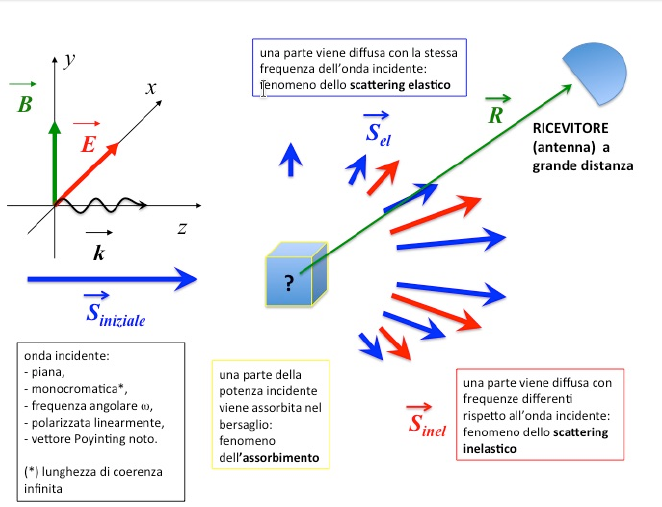
\includegraphics[width=0.4\textwidth]{immagini/1.png}
	\caption{Assobimento e diffusione e.m. di un sistema}
	\label{fig:1}
\end{figure}
Una parte della potenza irraggiata dall'onda sorgente può essere assorbita dall'oggetto (quindi dissipata con qualche meccanismo interno): fenomeno dell'assorbimento.\\
Una parte della potenza dell'onda incidente può essere diffusa sempre con la medesima frequenza: fenomeno della diffusione elastica.\\
Una parte della potenza dell'onda incidente può essere diffusa con frequenze differenti dalla incidente stessa: fenomeno della diffusione inelastica.\\
Un esempio di sistema di questo tipo è l'atomo in cui l'onda incidente eccita gli elettroni che, accelerando, possono irraggiare e dare luogo ai tre fenomeni citati.

\subsection[ Sezioni d'urto di onda E.M. su bersaglio]{Per un’onda e.m. monocromatica che incide su un bersaglio (per esempio un circuito o un atomo) definire le sezioni d’urto: di assorbimento, elastica differenziale, totale elastica; inelastica differenziale; inelastica totale; totale.}
\begin{itemize}
\item Sezione d'urto di assorbimento: 
	\[
		\sigma_{abs} = \frac{\left< P_{abs} \right> }{\left< \left|S_{in}\right| \right> }
	\] 	
\item Sezione d'urto elastica:
	\[
		\sigma_{el} = \frac{\left<P_{el} \right>}{\left< \left| S_{in} \right|  \right>} 
	\] 
	\[
		\frac{\mbox{d} \sigma_{el}}{\mbox{d} \Omega} = R^2 \frac{\left< \left| S_{el}\left( \theta,\phi \right)  \right|\right>}{ \left< \left| S_{in} \right|  \right> } 
	\] 
\item Sezione d'urto inelastica:\\
per ogni frequenza angolare $\omega_{i}$ a cui avviene la diffusione si ha:
\[
	\sigma_{\omega_{i}} = \frac{\left<P_{\omega_{i}} \right>}{\left< \left| S_{in} \right|  \right>} 
\] 
\[
	\frac{\mbox{d} \sigma_{\omega_{i}}}{\mbox{d} \Omega} = R^2 \frac{\left< \left| S_{\omega_{i}}\left( \theta,\phi \right)  \right|\right>}{ \left< \left| S_{in} \right|  \right> }
\] 
\item Sezione d'urto totale: 
	\[
	\sigma_{tot} = \sigma_{abs} + \sigma_{el} + \sum_{n=i} \sigma_{\omega_{i}}
	\] 
\end{itemize}
Da notare che l'unità di misura della sezione d'urto è quella di un'area.

\subsection[ Ampiezza di scattering]{Definire la ampiezza di scattering per un’onda e.m. monocromatica che incide su un bersaglio fisso (per esempio un circuito o un atomo).}
Per uno stato finale del sistema (con l'onda diffusa generata dal bersaglio) a grandi distanze il campo elettrico può esser scritto come il prodotto di un'onda sferica e di un termine che tenga conto della dinamicha del processo:
\[
	\boldsymbol{E}_{f} = \boldsymbol{f}\left( \theta, \varphi \right) \frac{e^{-i\left( \omega_{f}t - k_{f}R + \phi \right)}}{R}
\]
Con $\omega_{f}$ frequenza uscente, $k_{f}$ vettore d'onda uscente, $\phi$ fase.\\
L'ampiezza di scattering $\boldsymbol{f}$ è quindi l'ampiezza dell'onda sferica riemessa dall'oggetto scatterante (che interagisce con un'onda piana monocromatica). Questa è legata alla sezione d'urto differenziale dalla relazione:
\[
	\frac{\mbox{d} \sigma_{\omega_{f}}}{\mbox{d} \Omega} = \frac{\left| \boldsymbol{f}\left( \theta, \varphi \right) \right|^2}{\left| \boldsymbol{E_{0}} \right|^2 }
\] 


\subsection[ Potenza irraggiata da dipolo elettrico, magnetico e quadrupolo elettrico]{Descrivere la situazione in cui la legge 
\[
	P = \frac{2}{3c^3} \ddot{\boldsymbol{p_{e}}}^2 + \frac{1}{180 c^5} \dddot{Q_{ij}}^2 + \frac{2}{3c^3} \ddot{\boldsymbol{p_m}}^2
\] 
(espressa in CGS) è applicabile e spiegare il significato e l'unità di misura di ogni grandezza fisica ivi indicata; trascrivere poi l'espressione in MKSA.}
P è la potenza irraggiata da un sistema in cui sono presenti un dipolo elettrico (1), un quadrupolo magnetico (2) ed un dipolo magnetico (3):
\begin{enumerate}
	\item Dipolo elettrico:
	\[
		P_{1}^{CGS} = \frac{2}{3 c^3} \ddot{\boldsymbol{p}}_{el}^2 \quad \quad 
		P_{1}^{MKS} = k_{0}\frac{2}{3 c^3} \ddot{\boldsymbol{p}}_{el}^2
	\]
	con
	\[
		\boldsymbol{p}_{e} = \sum_{cariche} q \boldsymbol{r} 
	\] 
	\item Quadrupolo elettrico:
	\[
		P_{2}^{CGS} = \frac{1}{180 c^{5}}\dddot{Q_{ij}}^2 \quad \quad 
		P_{2}^{MKS} = k_{0} \frac{1}{180 c^{5}} \dddot{Q_{ij}}^2
	\]
	con
	\[
		\Q = \sum_{cariche}q\left( 3 \boldsymbol{r} \wedge \boldsymbol{r} - \boldsymbol{r}^2\I \right) 
	\] 
	\item dipolo magnetico:
	\[
		P_{3}^{CGS} = \frac{2}{3c^{3}} \ddot{\boldsymbol{p}}_{m}^2 \quad \quad 
		P_{3}^{MKS} = k_{0} \frac{2}{3c^5} \ddot{\boldsymbol{p} }_{m}^2
	\]
	con
	\[
		p_{m} = \frac{1}{2[c]} \sum_{cariche} q \boldsymbol{r} \wedge \boldsymbol{v}   
	\] 
\end{enumerate}
Queste sono applicabili se le dimensioni caratteristiche dell'oggetto che emette sono molto più piccole della lunghezza d'onda incidente. 


\subsection[ Distribuzione angolare della radiazione di dipolo elettrico e magnetico (non relativistico)]{Scrivere la distribuzione angolare della radiazione di dipolo elettrico e di dipolo magnetico nel caso non relativistico.}
\begin{figure}[H]
	\centering
	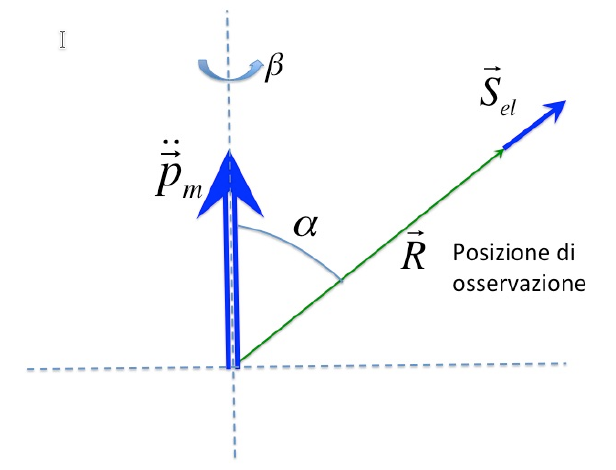
\includegraphics[width=0.4\textwidth]{immagini/2.png}
	\caption{Dipolo magnetico oscillante.}
	\label{fig:2}
\end{figure}
Sulla base della notazione di figura si ha:
\paragraph*{MKSA} I campi e la potenza irraggiata si scrivono come:\\
Dipolo magnetico:
\[
	\boldsymbol{E} = -k_{0}\frac{\ddot{\boldsymbol{p}}_m\left( t_{rit} \right) \wedge \hat{r} }{\left| \boldsymbol{r} \right| c^3} \quad \quad 
	\boldsymbol{B} = k_{0}\frac{\left( \ddot{\boldsymbol{p}}_{m}\left( t_{rit} \right) \wedge \hat{r}  \right) \wedge \hat{r}  }{ \left| \boldsymbol{r}  \right| c^3 }
\] 
\[
	P_m = \frac{\left| \ddot{\boldsymbol{p} }_{m} \right|^2}{6 \pi \epsilon_0 c^5} \quad  \quad \quad 
	\frac{\mbox{d} P_{m} }{\mbox{d} \Omega} = \frac{\mbox{d} P_m}{\mbox{d} \cos{\alpha \mbox{ d}\beta}} = \frac{1}{16 \pi ^2 \epsilon_0 c^5} \ddot{\boldsymbol{p}}_m^2( t_{rit})  \sin^2{\alpha} 
\] 
Dipolo elettrico:
\[	
	\boldsymbol{E} = k_{0}\frac{\left( \ddot{\boldsymbol{p}}_{e}\left( t_{rit} \right) \wedge \hat{r}  \right) \wedge \hat{r}  }{ \left| \boldsymbol{r}  \right| c^2 } \quad \quad 
	\boldsymbol{B} = k_{0}\frac{\ddot{\boldsymbol{p}}_e\left( t_{rit} \right) \wedge \hat{r} }{\left| \boldsymbol{r} \right| c^2} 
\] 
\[
	P_e = \frac{\left| \ddot{\boldsymbol{p} }_{e} \right|^2}{6 \pi \epsilon_0 c^3} \quad  \quad \quad 
	\frac{\mbox{d} P_{e}}{\mbox{d} \Omega} = \frac{\mbox{d} P_e}{\mbox{d} \cos{\alpha \mbox{ d}\beta}} = \frac{1}{16 \pi ^2 \epsilon_0 c^3} \ddot{\boldsymbol{p}}_e^2( t_{rit})  \sin^2{\alpha} 
\] 
\paragraph*{CGS} I campi e la potenza irraggiata si scrivono come:\\
Dipolo magnetico:
\[
	\boldsymbol{E} = -\frac{\ddot{\boldsymbol{p}}_m\left( t_{rit} \right) \wedge \hat{r} }{\left| \boldsymbol{r} \right| c^2} \quad \quad 
	\boldsymbol{B} = \frac{\left( \ddot{\boldsymbol{p}}_{m}\left( t_{rit} \right) \wedge \hat{r}  \right) \wedge \hat{r}  }{ \left| \boldsymbol{r}  \right| c^2 }
\] 
\[
	P_m = \frac{2}{3}\frac{\left| \ddot{\boldsymbol{p} }_{m} \right|^2}{c^3} \quad \quad \quad 
	\frac{\mbox{d} P_{m} }{\mbox{d} \Omega} = \frac{\mbox{d} P _m}{\mbox{d} \cos{\alpha \mbox{ d}\beta}} = \frac{1}{4 \pi c^3} \ddot{\boldsymbol{p}}_m^2( t_{rit})  \sin^2{\alpha} 
\] 
Dipolo elettrico:
\[	
	\boldsymbol{E} = \frac{\left( \ddot{\boldsymbol{p}}_{e}\left( t_{rit} \right) \wedge \hat{r}  \right) \wedge \hat{r}  }{ \left| \boldsymbol{r}  \right| c^2 } \quad \quad 
	\boldsymbol{B} = \frac{\ddot{\boldsymbol{p}}_e\left( t_{rit} \right) \wedge \hat{r} }{\left| \boldsymbol{r} \right| c^2} 
\] 
\[
	P_e = \frac{2}{3}\frac{\left| \ddot{\boldsymbol{p} }_{e} \right|^2}{c^3} \quad \quad \quad 
	\frac{\mbox{d} P_{e}}{\mbox{d} \Omega} = \frac{\mbox{d} P_e}{\mbox{d} \cos{\alpha \mbox{ d}\beta}} = \frac{1}{4 \pi c^3} \ddot{\boldsymbol{p}}_e^2( t_{rit})  \sin^2{\alpha} 
\]
Si potrebbe fare una verifica con: 
\[
	P = \int{ \frac{\mbox{d} P}{\mbox{d} \Omega}} \text{d}\Omega
\] 
\subsection[ Resistenza di irraggiamento per un circuito ad una maglia]{Definire la "resistenza di irraggiamento" di un circuito elettrico a una maglia e fornire un esempio.}
Nota la corrente ($I$) che scorre nel circuito la resistenza di irraggiamento è la resistenza dovuta alla dissipazione per irraggiamento:
\[
	R_{irr} = \frac{P_{irr}}{I^2}
\] 
Ad esempio per un circuito planare si ha (CGS):
\[
	\boldsymbol{m}  = IS \hat{n} / c \implies 
	R_{irr} = \frac{2}{3}\frac{S^2\omega^{4}}{c^{5}}
\] 

\subsection[ Urto elastico ed inelastico tra particelle con esempi]{Definire urto elastico ed urto inelastico fra due particelle; fornire poi almeno un esempio di reazione elastica ed una inelastica fra: 
	\begin{enumerate}
		\item un fotone ed un atomo
		\item due particelle cariche
		\item un protone ed un nucleo.
	\end{enumerate}
}
Un urto è elastico se la natura delle particelle non varia nell'urto stesso, ovvero se per ogni costituente
\[
	p^{\mu}_{i}p_{i,\mu} = m_{i}^2
\] 
è costante nel tempo. Urti di questo tipo sono della forma:
\[
	a \ + \ b \implies a \ + \ b
\] 
In tutti gli altri casi l'urto è anaelastico e si hanno situazion del tipo:
\[
	a \ + \ b \implies \sum_{i} p_{i}
\] 
Diamo adesso esempi di reazioni:
\paragraph{Fotone e Atomo}
\begin{itemize}
	\item Elastico: Scattering Thomson. 
	\[ 
		\gamma \ + \ H \implies \gamma \ + \ H 
	\]
	\item Inelastico: Effetto Compton.
	\[
		\gamma \ + \ A \implies \gamma \ + \ e^- \ + \ A^+
	\] 
\end{itemize}
\paragraph{Due particelle cariche}
\begin{itemize}
	\item Elastico: 
	\[
		p \ + \ p \implies p \ + \ p 
	\] 
	\item Inelastico: Produzione del bosone di Higs
	\[
		p \ + \ p \implies H \ + \ \ldots
	\] 
\end{itemize}
\paragraph{Protone e Nucleo}
\begin{itemize}
	\item Elastico: 
	\[
		\text{da trovare ancora\ldots}
	\]
	\item Inelastico: Reazione degli alchimisti
	\[
		p \ + \ {}^{198}_{80}\text{Hg}_{118} \implies p \ + \ p \ + \ {}^{197}_{79}\text{Au}^{-}_{118} 
	\] 
\end{itemize}
\subsection[ Conservazione di alcune grandezze per interazioni elettromagnetiche/forti]{Dire quali fra le seguenti grandezze si conservano sempre nei processi di urto in cui avvengano interazioni elettromagnetiche e/o forti, ma non deboli.} 
\begin{enumerate}
	\item \textbf{carica elettrica.} Si conserva.
	\item \textbf{numero barionico.} Si conserva.
	\item \textbf{numero leptonico elettronico.} Si conserva. 
	\item \textbf{numero leptonico muonico.} Si conserva.
	\item \textbf{numero di elettroni.} Non si conserva: Formazione di coppie.
		\[
			\ce{ \ce{\gamma} -> \ce{e^+} + \ce{e^-}}
		.\]  
	\item \textbf{differenza fra il numero di elettroni ed il numero di positroni.} Si conserva.
	\item \textbf{numero di protoni.} Non si conserva: produzione di protoni su nucleo.
	\item \textbf{differenza fra il numero di protoni ed il numero di antiprotoni.} Si conserva.
\end{enumerate}


\subsection[ Conservazione di alcune grandezze per interazioni forti]{Dire quali fra le seguenti grandezze si conservano sempre nei processi di urto in cui avvengano esclusivamente interazioni forti:  Fornire almeno un esempio per ogni situazione in cui vi sia una grandezza non conservata.}
\begin{enumerate}
	\item \textbf{carica elettrica.} Si conserva.
	\item \textbf{numero barionico.} Si conserva.
	\item \textbf{numero leptonico elettronico.} Si conserva.
	\item \textbf{numero leptonico muonico.} Si conserva.
	\item \textbf{numero di elettroni.} Si conserva.
	\item \textbf{differenza fra il numero di elettroni ed il numero di positroni.} Si conserva.  
	\item \textbf{numero di protoni.} Si conserva.
	\item \textbf{differenza fra il numero di protoni ed il numero di antiprotoni.} Si conserva.
\end{enumerate}


\subsection[$\ $ Conservazione di alcune grandezze per interazioni deboli]{Dire quali fra le seguenti grandezze si conservano sempre nei processi di urto in cui avvengano interazioni deboli, fornire almeno un esempio quando si ha qualcosa di non conservato.}
\begin{enumerate}
	\item \textbf{carica elettrica.} si conserva.
	\item \textbf{numero barionico.} si conserva.
	\item \textbf{numero leptonico elettronico.} non si conserva.
	\[
		\mu^- \implies e^- \ + \ \gamma
	\]
	\item \textbf{numero leptonico muonico.} Non si conserva, stessa interazione di sopra.
	\item \textbf{numero di elettroni.} Non si conserva: Decadimento del Neutrone.
	\[
		n \implies p \ + \ e^- \ + \ \overline{\nu}_{e}
	\] 
	\item \textbf{differenza fra il numero di elettroni ed il numero di positroni.} Non si conserva: Decadimento $\beta^+$
	\[	
		\ce{\ce{^{A}_{Z}X_{N}} -> \ce{^{A}_{Z-1}Y^{-}_{N+1}} + e^{+} + \nu_{e} }
	\] 
	\item \textbf{numero di protoni.} Non si conserva: Decadimento $\beta^-$
	\[
		\ce{\ce{^{A}_{Z}X_{N}} -> \ce{^{A}_{Z+1}Y^{+}_{N-1}} + e^{-} + \overline{\nu}_{e} }
	\] 
	\item \textbf{differenza fra il numero di protoni ed il numero di antiprotoni.} Non si conserva: Decadimento $\beta^-$ 
\end{enumerate}

\subsection[$\ $ Processi esclusivi e inclusivi, esotermici e endotermici, Q-value.]{Definire i processi esclusivi e inclusivi, il Q-valore di un processo e i processi esotermici o endotermici.}
Un processo si dice esclusivo se in esso viene misurato il 4-impulso di tutti i prodotti. Un processo si dice inclusivo se in esso vengono misurati solo i 4-impulsi di alcuni prodotti.\\
Il Q-valore di un processo è definito come: 
\[
	Q = \left( m_{i} - m_{f} \right) c^2 = T_f - T_i
\] \label{eq:Q-valore}
Un processo è esotermico se $Q > 0$, endoterimco altrimenti.

\subsection[$\ $ Tre definizioni di sezione d'urto equivalenti nei processi corpuscolari]{Definire la sezione d’urto nei seguenti tre casi, e dimostrare come da ognuno di essi si possano dedurre gli altri due: 
\begin{enumerate}
	\item Particelle incidenti su un unico bersaglio [dati: $j_{\text{incidenti}}$; $N_f$] 
	\item Sottile fascio di particelle incidenti su una lastra contenente i bersagli [dati: $\Phi_{incidenti}$, $\hat{\sigma}_{bersagli}$, $N_f$] 
	\item Urti nel volume fra particelle di due specie diverse e differenti concentrazioni [dati: $N_{eventi}$ per unità di tempo e di volume, $n_1$ e $n_2$ concentrazione delle particellle interagenti, $v_{rel}$ (si ipotizza che tutte le particelle di una specie abbiano la stessa velocità).]
\end{enumerate}
Con $\hat{\sigma}$ densità superficiale di eventi,  $j$ densità di corrente, $N_f$ frequenza di eventi osservati (o numero di eventi per unità di tempo),  $\Phi$ flusso di particelle. 
}
Nel primo caso si ha:
\[
	\sigma = \frac{1}{\left| \boldsymbol{j}\right|} \frac{\mbox{d} N_{f}}{\mbox{d} t} 
\] 
Nel secondo invece:
\[
	\sigma = \frac{1}{n_s \Phi} \frac{\mbox{d} N_f}{\mbox{d} t} 
\] 
Nel terzo:
\[
	\sigma = \frac{1}{n_1 n_2 v_{rel}} \frac{\mbox{d} n_f}{\mbox{d} t} 
\] 
Nell'ultimo la sezione d'urto dipende dalla velocità relativa. Inoltre se si ha la funzione di distrubuzione per la velocità relativa:
\[
	\frac{\mbox{d} N_f}{\mbox{d} t} = n_1 n_2 \int_0^\infty \sigma\left( v_{rel} \right) f\left( v_{rel} \right) dv_{rel}
\] 
Per passare dal primo al secondo caso basta osservare che:
\[
	\Phi = \left| \boldsymbol{j} \right| S, \quad \quad 
	n_{s} = \frac{1}{S} \quad \left( \text{un bersaglio} \text{} \right) 
\] 
Con S area del bersaglio.
Se mi metto in un sistema in cui una delle particelle è ferma, è evidente mostrare l'equivalenza tra il caso (2) e (3).

\subsection[$\ $ Sezione d'urto elastica, inclusiva, esclusiva e totale per urti tra particelle]{Per gli urti fra due particelle definire le sezioni d'urto: elastica, inelastica, inclusiva, esclusiva, totale.}
Consideriamo la reazione:
\[
	a \ + \ b \implies p_1 \ + \ p_2 \ + \ \ldots \ + \ p_n
\] 
e sia $f_i\left( E_i \right) $ la distrubuzione di probabilità dell'energia del prodotto i-esimo. La sezione d'urto inclusiva di tale prodotto è:
\[
	\sigma_i = \int_{E_{i, min}}^{E_{i,max}} f\left( E_{i} \right) dE_{i}
\]
Se invece si considera la distribuzione degli impulsi di tutte le particelle finali: $f\left( P_{1}, \ldots , P_{n} \right) $ si ha una sezione d'urto esclusiva:
\[
	\sigma_e = \int f\left( P_{1}, \ldots P_{n} \right) \prod_{i = 1}^{n}d^{4}P_i  
\] 
La sezione d'urto elastica è la sezione d'urto reltiva as un urto elastico, la sezione d'urto anaelastica è la sezione d'urto relativa ad un urto anaelastico.

\subsection[$\ $ Probabilità di interazione di particella su lamina sottile]{Calcolare la probabilità di interazione per una particella che incide su una lamina sottile [dati: $\sigma$ processo, $N_{bersagli}$ per unità superficie].\\
Che significato avrebbe una probabilità maggiore di uno? Quest'ultima risposta dipende dalle tipologie degli urti?}
La probabilità di interazione è: $P = N \sigma $. Se  questa è maggiore di 1 significa che è venuta meno l'approssimazione di lamina sottile. In ogni caso questa non dipende dal tipo di interzaione.

\subsection[$\ $ Forza di reazione radiativa]{Indicare le condizioni per cui la forza di reazione radiativa per una particella (di massa m e carica unitaria) $F_{rad} = m \tau \dot{\boldsymbol{a}}$ è da considerarsi valida ed utilizzabile.} \label{subsec: 2.a.15}
Si ritiene necessario, per indicare le approssimazioni, ricavare la forza in questione. 
La forza di radiazione può essere defita come la forza il cui lavoro è responsabile della perdita di energia per irraggiamento noto nella formula di Larmor (CGS):
\[
	\int_{t_1}^{t_2} \boldsymbol{F}_{rad} \cdot \boldsymbol{v} dt = -\frac{2}{3} \frac{e^2}{c^3} \int_{t_1}^{t_2} \dot{\boldsymbol{v}}^2
\]
Posso scrivere:
\[
	\dot{\boldsymbol{v}}^2 = \frac{\mbox{d} \left( \boldsymbol{v} \dot{\boldsymbol{v}} \right) }{\mbox{d} t} - \boldsymbol{v} \ddot{\boldsymbol{v}} 
\]
Inserendo nel secondo membro della equazione si ha:
\[
	\int_{t_1}^{t_2}{ \boldsymbol{F_{rad}} \cdot \boldsymbol{v} dt } = -
\left. \frac{2}{3}\frac{e^2}{c^3} \boldsymbol{v} \cdot \dot{\boldsymbol{v}}\right|_{t_{1}}^{t_{2}} + \frac{2}{3}\frac{e^2}{c^3} \int_{t_1}^{t_2} \boldsymbol{v}  \cdot \ddot{\boldsymbol{v}} dt
\] 
Se il moto è periodico di ha: 
\[
	\int_{t_1}^{t_2} \left( \boldsymbol{F}_{rad} - \frac{2}{3}\frac{e^2}{c^3}\ddot{\boldsymbol{v}} \right) \cdot \boldsymbol{v} dt = 0  
\] 
Poiche velocità e accelerazione sono ortogonali in tal caso, abbiamo quindi un candidato per la $\boldsymbol{F}_{rad}$.
\[
	\boldsymbol{F}_{rad} = \frac{2}{3}\frac{e^2}{c^3} \ddot{\boldsymbol{v}}.  
\] 
che in MKSA si scrive come:
\[
	\boldsymbol{F}_{rad} = \frac{q^2}{6\pi \epsilon_0 c^3} \dddot{\boldsymbol{x}} = m_{e}\frac{q^2}{6\pi \epsilon_0 c^3} \dddot{\boldsymbol{x}} = m_e \frac{2}{3}\frac{r_e}{c} \dddot{\boldsymbol{x}} = m_e \tau \dddot{\boldsymbol{x}} 
.\] 
Possiamo quindi dare una stima dei valori tipici di questa forza:
\[
r_e = \frac{q^2}{4\pi \epsilon_0 m_e c^2} = 2.82 fm \implies \tau = \frac{2}{3}\frac{r_e}{c} = 6.2 \cdot 10^{-24} s 
.\] \label{eq: raggio classico} 
Tenendo conto della forza viscosa che agisce classicamente sull'elettrone 
\[
	\boldsymbol{F}_{visc} = -\beta \dot{\boldsymbol{x}} = - m_e \Gamma' \dot{\boldsymbol{x}} 
\]
con valori tipici: $\Gamma' \sim 10^{10} \ s^{-1}$.\\
Infine ipotizzando anche una forza "elastica" attrattiva nucleare con valore tipoco $\omega_{0} \sim 10^{14} - 10^{16}$ otteniamo la relazione:
\[
\Gamma' \ll \omega_{0} \ll \frac{1}{\tau}
.\] \label{eq:relazione-parametri-elettrone} 
Questo conto sarà utile per la Domanda \hyperref[subsec: 2.b.12]{2.b.12}.

\subsection[$\ $ Significato fisico della Breight-Wiegner]{Spiegare il significato e indicare l'unità di misura di ogni grandezza fisica nelle seguenti leggi:
\[
	\left( 1 \right) \to \frac{\mbox{d} \sigma_{el}}{\mbox{d} \Omega} = r_{e}^2 L \left( \omega \right)  \sin^2 \left( \alpha \right)   \quad \quad
	\left( 2 \right) \to  \frac{\mbox{d} \sigma_{el}}{\mbox{d} \Omega} = r_{e}^2 L \left( \omega \right)  \frac{1 + \cos^2 \left( \alpha \right) }{2}   
\]
\[
	\left( 3 \right) \to  \sigma_{el} = \sigma_{Th} L \left( \omega \right) \quad \quad 
	\left( 4 \right) \to  \sigma_{tot} = 4 \pi r_{e} c \frac{\omega^2 \Gamma }{\left( \omega_{0}^2 - \omega^2 \right)^2 + \omega^2 \Gamma_{tot} } 
\] 
con 
\[
	L \left( \omega \right) = \frac{\omega^4}{\left( \omega_{0}^2 - \omega^2 \right)^2 + \omega^2 \Gamma_{tot} } \quad \quad 
	\sigma_{Th} = \frac{8}{3} \pi r_{e}^2 = 0.66 \text{ barn}
\]
inerenti l'interazione di un’onda e.m. piana e monocromatica su un elettrone legato elasticamente.} \label{subsec: 2.a.16}
L'equazione (1) è la sezione d'urto differenziale per l'interazione tra l'elettrone ed un onda polarizzata linearmente. Può essere ottenuta dalla equazione del moto dell'elettrone legato elasticamente soggetto alle forze della domanda precedente (di richiamo, di attrito viscoso e radiazione radiativa) immerso nel campo di una onda e.m. piana monocromatica (vedi Domanda \hyperref[subsec: 2.b.12]{2.b.12}):
\[
	\boldsymbol{x} = \frac{e \boldsymbol{E_0}}{m_e}\frac{1}{\omega_0^2-\omega^2- i\omega \Gamma' - i \tau \omega^2} = \frac{eE_0}{m_e}\frac{1}{\omega_0^2-\omega^2- i\omega\Gamma_{tot}}
.\] 
In cui si definiscono 
\[
	\Gamma_{tot} = \Gamma' + \Gamma \frac{\omega^2}{\omega_0^2} \quad \quad 
	\Gamma = \omega_0^2 \tau \quad \text{ con $\tau$ quello ottenuto nella domanda precedente}
\]
Quindi basta adesso ricordare che la distribuzione angolare di potenza irraggiata da un dipolo oscillante $ \boldsymbol{p} = \boldsymbol{p}_0 e^{-i\omega t}$ è:
\[
	\frac{\mbox{d} P}{\mbox{d} \Omega} = \frac{\omega^{4} \left| \boldsymbol{p}_0 \right|^2 }{4\pi c^3} \sin^2\left( \alpha \right) 
.\] 
Quindi inserendo $\left| \boldsymbol{p}_0 \right| = \left| e \boldsymbol{x} \right| $  e dividendo per il vettore di Poynting incidente si ha la tesi (1).

L'equazione (2) è la sezione d'urto differenziale con l'onda incidente non polarizzata: bisogna in questo caso mediare su tutte le possibili polarizzazioni dell'onda incidente ottendendo il fattore finale.\\
l'espressione (3) si ottinene integrando sull'angolo solido la (1) o la (2).\\
infine la (4) è la sezione d'urto totale definita come:
\[
	\sigma_{tot} = \frac{e \left< \dot{\boldsymbol{x}}\boldsymbol{E}\right>}{\left<\boldsymbol{S_{in}} \right>}
.\]
Possiamo notare anche che:
\[
	\frac{\sigma_{el}}{\sigma_{tot}} = \frac{1}{1 + \Gamma'/\left( \omega^2\tau \right)  }
.\] 
Che tende all'unità quando non c'è dissipazione.

\subsection[$\ $ osservazioni sullo scattering Rutherford]{Discutere qualitativamente le osservazioni sperimentali dello scattering di Rutherford.}
Inviando un fascio di particelle $\alpha$ su una lamina d'oro si osserva che circa 1 particella su 8000 viene deviata a grandi angoli o rimbalza. Queste osservazioni non sono spiegabili con il modello a panettone di Thomson ma si spiegano bene con il modello di Bhor.
\[
	\left. \frac{\mbox{d} \sigma}{\mbox{d} \Omega} \right|_{Ruth} = \frac{1}{\left(4\pi \epsilon_0\sin^{2}\left( \frac{\theta}{2} \right) \right)^2 } \left(\frac{zZe^2}{4T} \right)^2 
.\] 
Si deduce facilmente che le particelle più energetiche sono più penetranti, le particelle più cariche vengono maggiormente deflesse.

\subsection[$\ $ Differenza tra Scattering Rutherford e Mott]{Spiegare la differenza fra lo scattering Rutherford e lo scattering Mott.}
Lo Scattering Mott:
\[
	\left. \frac{\mbox{d} \sigma}{\mbox{d} \Omega} \right|_{Mott} = \left. \frac{\mbox{d} \sigma}{\mbox{d} \Omega} \right|_{Ruth} \left( 1- \beta^2 \sin^2\left( \frac{\theta}{2} \right)  \right) 
.\] 
Tiene conto dello spin degli elettroni e degli effetti relativistici che questi hanno nel loro moto.

\subsection[$\ $ Significato dei termini nelle sezioni d'urto Mott e Rutherford]{Spiegare il significato di tutti i termini delle seguenti espressioni delle sezioni d’urto differenziali Rutherford e Mott: 
\[
	\left. \frac{\mbox{d} \sigma}{\mbox{d} \Omega} \right|_{Ruth} = \left( \frac{zZe^2}{4 \pi \epsilon_0} \right)^2 \left( \frac{1}{4T} \right)^2 \frac{1}{\sin^4\left( \theta/2 \right) }  
\] 
\[
	\left. \frac{\mbox{d} \sigma}{\mbox{d} \Omega} \right|_{Mott} = \left. \frac{\mbox{d} \sigma}{\mbox{d} \Omega} \right|_{Ruth} \left( 1 - \beta^2 \sin^2 \theta/2  \right) \quad \quad
	\text{con } T \to \frac{pV}{2}
\] 
}
Sono tutti termini di banale comprensione, ricordiamo però che $\theta$ è l'angolo di scatterig: l'angolo tra la direzione iniziale della particella e quello finale.

\subsection[$\ $ Definizione di raggio nucleare tramite lo Scattering Rutherford]{Dare la definizione operativa di raggio nucleare mediante lo scattering di Rutherford.}
Fissando un angolo di scatternig $\hat{\theta} = 60^o$ si ha che per energie maggiori di $T_{soglia} \approx 30 MeV$ divena importante l'interzione forte con il nucleo: si ha un discostamento dalla legge che lega la sezione d'urto Rutherford a T. Quindi possiamo ipotizzare che la distanza minima che si ottiene in questo caso sia una buona stima del raggio nucleare.
\[
	d \approx \frac{zZ e^2}{4 \pi \epsilon_0 T_{soglia}} \implies R = \frac{d}{2}\left( 1 + \frac{1}{\sin\left( \frac{\hat{\theta}}{2} \right) } \right) 
.\] 
È necessario notare che $R$ è la distanza tra i nuclei degli atomi coinvolti nello scattering, non il nucleo dell'atomo (che vorremmo definire), è quindi necessario incidere con particelle il cui nucleo sia di dimensioni attese molto inferirori rispetto a quelle del nucleo in esame per dare una buona stima del raggio di quest'ultimo (ipotesi verificata nel caso di particelle $\alpha$ su Piombo, ad esempio).

\subsection[$\ $ Definizione di A, Z, N, nuclei isotopi, isobari, isotoni, stabili ed instabili]{Definire le quantità che in un nucleo usualmente si indicano con A, Z, N (simbologia ${}^A_Z X_N$ ). Dare la definizione di nuclei isotopi, isobari, isotoni, stabili, instabili.}
A è il numero di nucleoni (protoni e neutroni), Z è il numero di protoni, N è il numero di neutroni.\\
Due nuclei sono:
\begin{itemize}
	\item Isotopi: hanno lo stesso Z.
	\item Isobari: hanno lo stesso A.
	\item Isotoni hanno lo stesso N.
	\item Instabili: hanno vita media finita.
	\item Stabili: hanno vita media "infinita".
\end{itemize}

\subsection[$\ $ Unità di massa atomica, energia di legame B e difetto di massa $\Delta$]{Dopo avere definito l’unità di massa atomica e avere dato il suo valore in MeV/$c^2$, definire l’energia di legame (B) di un atomo ed il “difetto di massa” ($\Delta$) di un atomo.}
\[
	\text{1 u.m.a.} = \frac{1}{12}m\left( {}^{12}_{6}C_{6} \right) = 931.49 \text{ MeV/}c^2 
.\]
La B è l'energia necessaria per separare un nucleone dal suo nucleo.\\
L'energia di legame B di un nucleo X con A nucleoni e Z protoni è:
\[
	B\left( A, Z \right) = Z\left( m_p + m_e - m_u \right) - N \left( m_n - m_u \right) - \Delta_{A, Z} = 7.29 \text{MeV} \cdot Z + 8.07 \text{MeV} \cdot N - \Delta_{A,Z} 
.\] 
Dove 
\[
	m_u = 1 \text{ u.m.a.}\quad \quad 
	m_p = 938.2 \text{ MeV/}c^2\quad \quad 
	m_e = 0.511 \text{ MeV/}c^2
\]
Il difetto di massa è invece:
\[
	\Delta = m_{x} - \frac{A}{12}m\left( {}^{12}_{6}C_{6} \right) = m_x - Am_u 
.\] 
E lo si pio trovare nelle tabelle in rete.\\
Il difetto di massa è particolarmente utile per ricavare il Q-valore: è immediato esprimere la massa del nucleo coinvolto in una interazione mediante tale quantita e l'unità di massa atomica $m_u$.

\subsection[$\ $ Formula semiempirica B e termini spiegati dal modello a goccia]{Enunciare la formula semiempirica B = B(A,Z) ed indicare i suoi termini che sono spiegati dal modello a goccia. Spiegare le ipotesi su cui tale modello è basato e
fornire l'ordine di grandezza dell’energia media di legame di un nucleone all’interno di un nucleo.}
Nel modello a goccia si ha in prima approssimazione (per nuclei abbastanza grandi) una energia di legame proporzionale al numero di nucleoni e quindi al volume del nucleo stesso:
\[
	B_1\left( A, Z \right) = a_V A \quad \quad \text{Termine correttivo di volume}
.\] 
In seconda approssimazione possiamo considerare che i nucleoni che si trovano sulla superficie del nucleo non sono circondati da altri nucleoni, vi sarà allora un termine correttivo superficiale:
\[
	B_2\left( A,Z \right) = a_S A^{2/3} \quad \quad \text{Termine correttivo di superficie} 
.\] 
Poi possiamo aggiungere una ulteriore correzione per tener conto della repulsione columbiana tra i nucleoni carichi (Z tiene conto della carica, A tiene conto del raggio):
\[
	B_3\left( A,Z \right) = a_C \frac{Z^2}{A^{2/3}} \quad \quad \text{Termine correttivo Columbiano}
.\] 
Si hanno infine altri termini correttivi che tengono di conto di effetti quantistici e del principio di Pauli:
\[
	B\left( A,Z \right) = a_{V}A - a_{S}A^{2/3} - a_{C} \frac{Z^2 }{A^{1/3}} + a_{sym}\frac{\left( Z - N \right)^2}{A} + \delta_{pair} 
.\] \label{eq:B-energy}
Il modello in considerazione è quello "A Goccia", l'ipotesi di questo è che il nucleo di numero atomico Z e peso atomico A occupi un volume sferico di raggio:
\[
	R = r_0 A^{1/3} + r_{skin} \approx \left( 1.25 A^{1/3} + 2.0  \right) fm
.\]
Il modello prevede che l'energia di legame tra due nucleoni sia dell'ordine di $\sim 2.2$ MeV, ovvero la differenza tra la massa del deutone e la somma delle masse del protone e neutrone. 

\subsection[$\ $ Definizione dei decadimenti $\alpha$, $\beta^{+}$,$\beta^{-}$, $\gamma$, cattura elettronica con rispettivi Q-Value]{Definire i decadimenti $\alpha$, $\beta$ , $\gamma$ e il decadimento tramite cattura elettronica in un nucleo. Calcolare il Q-valore per il decadimento $\beta+$, $\beta-$, e per la cattura elettronica a partire dal difetto di massa delle specie coinvolte.} \label{sec:decadimenti}
\paragraph{Decadimento $\alpha$}
\[
	\ce{ \ce{^{A}_{Z}X_{N}} -> \ce{^{A-4}_{Z-2}Y^{2-}_{N-2} + \alpha}} \quad \quad \text{con $\alpha$ nucleo di  \ce{^{4}_{}He^{2+}_{}}}
\]
\paragraph{Decadimento $\beta+$}
\[
	\ce{\ce{^{A}_{Z}X_{N}} -> \ce{^{A}_{Z-1}Y^{-}_{N+1}} + e^{+} + \nu_{e} }
.\]
in cui si ha la transizione:
\[
	\ce{p -> n + e^+ + \overline{\nu}_e}
.\]
Il Q-valore del decadimento è : $Q = \Delta_{A,Z} - \Delta_{A, Z-1} - 2m_e $\\
Il Q-valore della reazione è: $ Q = m_p - m_n - m_e = - 1.804 $MeV.

\paragraph{Decadimento $\beta-$}
\[
	\ce{\ce{^{A}_{Z}X_{N}} -> \ce{^{A}_{Z+1}Y^{+}_{N-1}} + e^{-} + \overline{\nu}_{e} }
.\]
in cui si ha la transizione:
\[
	\ce{n -> p + e^- + \nu_e}
.\]
Il Q-valore del decadimento è : $Q = \Delta_{A,Z} - \Delta_{A, Z+1} $\\
Il Q-valore della reazione di transizione è: $ Q = m_n - m_p - m_e = 0.782 $MeV.
\paragraph{Cattura elettronica}
\[
	\ce{\ce{^{A}_{Z}X_{N}} -> \ce{^{A}_{Z-1}Y_{N+1}} + \nu_e} \quad \quad Q = \Delta_{A,Z} - \Delta_{A, Z-1} 
.\] 
in cui si ha:
\[
\ce{p + e ->n + \nu_e }
.\] 

\subsection[$\ $ Scoperta del neutrino nel decadimento $\beta^{-}$]{Come si e' arrivati alla conclusione che nel decadimento beta deve essere emessa una particella neutra non rivelata? }
Il problema in questione risale al 1934 (con Pauli che ipotizza l'esistenza della particella), venne formalizzato successivamente da Fermi e da Bhor.\\
Ciò che destava sgomento era lo spettro di emissione dell'elettrone. Spieghiamo a grandi linee il problema: \\
All'inzio si pensava che avvenisse il processo
\[
	\ce{n -> p + e-}
.\] 
In cui sicuramente si hanno le relazioni (di qui in avanti c = 1) 
\[
	m_e \text{ (0.511 MeV) }\ll m_p \text{ (938.3 MeV) } \approx m_n \text{ (939.6 MeV)}
.\] 
Conviene quindi ipotizzare che il neutrone si trovi inizialmente fermo, in tal caso anche il protone viene praticamente creato fermo. Per la conservazione dell'energia:
\[
	m_n =E_p + E_e
.\]
con 
\[
	E_p = \sqrt{m_p^2 + p_p^2} \quad \quad 
	E_e = \sqrt{m_e^2 + p_e^2} 
.\]
Se si trascura il rinculo del protone, come ipotizzato sopra:
\[
	m_n \approx m_p + \sqrt{m_e^2 + p_e^2} 
.\]
Quest'ultima relazione fissa l'impulso e l'energia dell'elettrone, quindi ci aspettiamo che lo spettro di quest'ultimo abbia un unico picco, invece sperimentalmente si ottengono curve del tipo:
\begin{figure}[H]
	\centering
	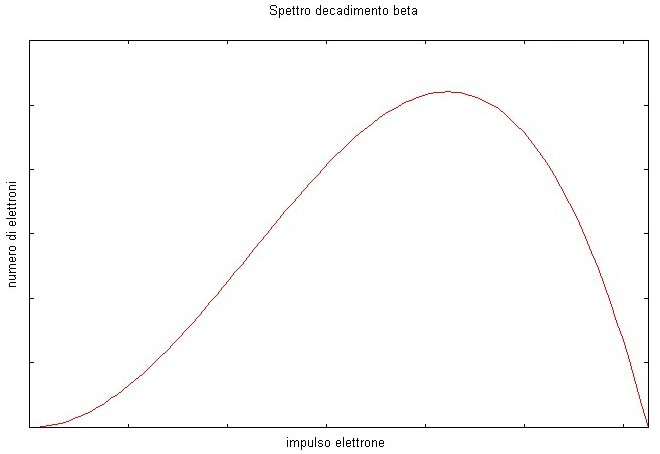
\includegraphics[width=0.5\textwidth]{immagini/Decadimento_beta_(spettro).jpg}
	\caption{Spettro di energia dell'elettrone.}
	\label{fig:beta}
\end{figure} 
Tale grafico mostra uno spettro completo che parte da energie nulle fino ad arrivare ad annullarsi di nuovo a $\sim 5.5 \ m_e$.\\
Per spiegarlo è quindi necessario ipotizzare che vi sia un'altra particella tra i prodotti che è appunto il neutrino.


\subsection[$\ $ Spiegazione dell'esistenza del neutrone nell'atomo]{Spiegare perchè, sebbene il neutrone libero sia instabile, esso non possa decadere quando è all'interno di taluni nuclei.}
Affinchè il neutrone in un nucleo possa decadere è necessario che
\[
	Q = \sum_{in} M_k - \sum_{fin} M_k > 0
.\] 
Questo in alcuni nuclei può non essere verificato, ad esempio:
\paragraph{Stabilità del Deuterio}
\[
	\ce{\ce{^{2}_{1}H_{1}} -> \ce{^{1}_{1}H_{0}} + p + e- + \overline{\nu}_e }
.\] 

con:
\[
	\ce{n -> p + e- + \overline{\nu}_e}
.\] 
si ha che la reazione non avviene perchè: 
\[
	Q = \Delta_{2,1} - 2\Delta_{1,0} = (13.136 -14.578)\text{ MeV} = -1.442 \text{ MeV} 
.\] 

\subsection[$\ $ Particelle per la misura del fattore di forma]{Quali particelle incidenti e di quale energia si utilizzano per misurare i fattori di forma nucleari?}
Si usano in genere Scattering elastici, in particolare la particella adatta è l'elettrone, ad esempio:  
\[
\ce{e- + p  -> e- + p} \quad \quad \text{Per misurare il fattore di forma e.m. del protone}
.\] 
Se funziona con il protone allora funziona anche con i nuclei avendo cura di scegliere le giuste energie con il metodo seguente.\\
Per quanto riguarda l'energia dell'elettrone dobbiamo tener di conto di che lunghezza vogliamo ispezionare: Per sondare oggetti di dimensioni caratteristiche del fm è necessario sondare con energie aventi le stesse dimensioni in termini di lunghezza d'onda di De Broglie:
\[
	E = \hbar \omega = \frac{2\pi\hbar c}{\lambda} =  \frac{1240 \text{ MeV} \cdot \text{fm}}{1 \text{ fm}} = 1240 \text{ MeV}
.\]

\subsection[$\ $ Larghezza di vita media, tempo di dimezzamento, branching fraction]{Dare le definizioni di: larghezza, vita media, semivita (o tempo di dimezzamento), rapporto di decadimento (“Branching fraction” o “Branching ratio”) per il decadimento di una particella.}
Se N è il numero di particelle non ancora decadute la vita media è definita da:
\[
	\dot{N} = -\frac{N}{\tau}
.\] 
La larghezza di vita media è la probabilità di decadimento nell'unità di tempo:
\[
	\Gamma = 1/\tau
.\]
La larghezza viene solitamente espressa in eV tramite:
\[
	\Gamma \text{ [eV]} = \Gamma \text{ [s]}^{-1} \cdot \hbar
.\] 
Perchè una particella che decade si può interpretare come una risonanza piccata nella massa di quest'ultima e di larghezza prorio $\Gamma$.\\
Il tempo di dimezzamento è
\[
	T = \tau \ln\left( 2 \right)  
.\] 
In fine il rapporto di decadimento di un "canale" è il rapporto tra i decadimenti di quel canale ed il numero totale di decadimenti.
\[
	B_{\text{f}} = \frac{\Gamma_{\text{f}}}{\Gamma}
.\] 

\subsection[$\ $ Ordini di grandezza di sezioni d'urto forti o deboli]{ Quali sono gli ordini di grandezza tipici delle sezioni d’urto delle interazioni forti e delle interazioni deboli?}
Per le interazioni forti si hanno sezioni d'urto dell'ordine di $10 - 100$ mb, per le interazioni deboli invece $1$ fb.

\subsection[$\ $ Vite medie per interazioni forti, elettromagnetiche, deboli]{Quali sono, approssimativamente, gli ordini di grandezza delle vite medie dovute ad interazioni deboli, elettromagnetiche, forti?}
\begin{itemize}
	\item Interazioni deboli: dai 15 minuti per il decadimento $\beta$ del neutrone fino a $10^{-8}$ s del decadimento del  $\pi$ carico.
	\item Interazioni eletromagnetiche: tempi tipici sono dell'ordine di $10^{-16}$ s.
	\item Interazione forte: tempi tipici sono $10^{-23}$ s.
\end{itemize}

\subsection[$\ $ Cinematica dell'effetto Mossbauer]{Spiegare la cinematica di un decadimento $\gamma$ nucleare e spiegare qualitativamente l'effetto Mossbauer. }
\paragraph{Definizione di decadimento $\gamma$.}
I decadimenti $\gamma$ sono delle transizioni fra uno stato eccitato di un nucleo ed uno stato di energia inferiore con l'emissione di un fotone (raggi X: 10keV-1MeV).\\
Considerando la reazione:
\[
	\ce{\ce{^{57}_{26}F^*_e} ->[T_{1/2} = 97.7 \text{ ns}] \ce{^{57}_{26}F_e} + \gamma ( 14.4 \text{ keV} ) }
.\] 
\begin{itemize}
	\item $M$: la massa dello stato fondamentale del nucleo.
	\item $M^* = M + E_0$ : la massa dello stato eccitato. 
	\item $E_\gamma$: l'energia del fotone nel laboratorio e nel centro di massa se il decadimento avviene da fermo.	
\end{itemize}
Siamo interessati all'energia dei fotoni uscenti, a prima vista sembrerebbe $E_0$ ma in realtà è una sovrastima: il rinculo del nucleo si porta via energia, vediamolo cinematicamente.\\ 
La quantità di moto del fotone nel centro di massa (e quindi anche dell'atomo di $F_e$):
\[
	E_\gamma = P^\gamma_{cm}
.\] 
Quindi si ha anche che dalla conservazione dell'energia:
\[
	E_{in} = M^* = M + E_0 = E_{fin} = \sqrt{M^2 + E_\gamma^2} + E_\gamma 
.\]
Possiamo quindi ricavare $E_\gamma$ in funzione di tutto il resto:
\[
	E_\gamma = \frac{E_0\left( E_0 + 2M \right)}{2\left( E_0 + M \right)} 
.\]
Essendo la massa del $\ce{^{57}_{26}F_e} = 53.05 \text{ GeV}$ ed $E_0 = 14.4 \text{ keV}$ possiamo approssimare:
\[
	E_\gamma  \approx E_0 - \frac{E_0^2}{2M}
.\] 
Quindi l'energia persa è:
\[
	\Delta E_\gamma \approx - \frac{E_0^2}{2M} \implies \frac{\Delta E_\gamma}{E_\gamma} \approx - \frac{E_0}{2M}  
.\]
Essendo $E_0 \approx E_\gamma$. Nel caso in esame si ha:
\[
	\left| \Delta E_\gamma \right| \approx 1.9 meV \implies \left| \frac{\Delta E_\gamma}{E_\gamma}\right| \approx 1.3 \cdot 10^{-7} 
.\] 
Quest'ultima è molto maggiore di:
\[
	\frac{\Gamma}{E_0} = 3.2 \cdot 10^{-13} 
.\] 
Quindi sarà difficile che un fotone partito dal decadimento riesca ad eccitare un nuovo atomo di $F_e$ poichè il fotone è emesso in un range di energia molto grande rispetto alla larghezza del processo.\\
Se invece prendo un blocco di atomi di ferro (o in gergo: nu bll pezz de ferragl) la massa che va al denominatore nelle equazioni sopra non è più quella del singolo atomo ma quella di tutto il blocco. Succede quindi che:
\[
	\Delta E_\gamma \ll \Gamma 
.\] 
Si può quindi avere un effetto coerente se il fotone che esce urta contro un altro atomo di ferro: Effetto Mosbauer.

\subsection[$\ $ Variabili indipendenti con due reagenti e N prodotti]{Quante sono le variabili indipendenti nello stato finale di una reazione in cui due particelle collidono ed N particelle sono prodotte?}
Sia il processo di decadimento:
\[
	\ce{a + b -> p_1 + p_2 + \ldots \text{+} p_n }
.\] 
Si ha che il numero di osservabili indipendenti è dato da le variabili ed i vincoli in gioco:
\begin{itemize}
	\item n 4-impulsi $\implies$ 4n variabili
	\item n vincoli dovuti alla massa delle singole particelle: $m_i^2 = P_{0, i}^2 - \boldsymbol{P}_{i}^2$
	\item 4 vincoli per la conservazione impulso-energia: $P_{in} = \sum_i P_i$
\end{itemize}
quindi le variabili indipendenti sono 3n - 4.
\paragraph{Nota}%
In quanto affermato non c'è stato bisogno di esplicitare il numero di reagenti, questo numero vale in generale per qualsiasi numero di particelle iniziali (se si hanno n prodotti).

\subsection[$\ $ Variabili indipendenti per un decadimento a due, considerazioni sul caso di Spin nullo]{Quante sono le variabili indipendenti nello stato finale di una reazione in cui una particella decade in due particelle? Quali implicazioni avremmo se la particella che decade avesse un momento angolare nullo? }
Le variabili indipendenti sono 3*2 - 4 = 2, se la particella ha spin nullo allora si ha una isotropia spaziale che ci permette di integrare l'espressione per il decadimento a due corpi:
\[
	\frac{\mbox{d} \Gamma}{\mbox{d} \Omega_1} = f_{dec}\left( \Omega_1 \right) \frac{P_{cm}}{4M} 
.\] 
sull'angolo solido:
\[
	\Gamma = f_{dec} \frac{P_{cm}}{4M}4\pi
.\] 

\subsection[$\ $ Variabili del Dalitz Plot]{Definire le variabili utilizzate nel "Dalitz plot".}
Le variabili del Dalitz plot sono:
\begin{itemize}
	\item $s_{12}$: il quadrato della massa invariante delle particelle 1 e 2
	\item $s_{23}$: il quadrato della massa invariante delle particelle 2 e 3
\end{itemize}

\subsection[$\ $ Variabili indipendenti per il decadimento a tre corpi, considerazioni sul caso di Spin nullo]{Quante sono le variabili indipendenti nello stato finale di una reazione in cui una particella decade in tre particelle? Quali implicazioni avremmo se la particella che decade avesse un momento angolare nullo?}
Le variabili indipendenti sono 3*3-4 = 5.\\
La larghezza di decadimento si può esprimere come:
\[
	\Gamma = \int{f_{dec}\left( s_{12}, s_{23}, \alpha ,\beta,\gamma \right) dL_p}
.\] 
Con $\alpha, \beta,\gamma$ angoli di Eulero e $dL_p$ elemento infinitesimo dello spazio delle fasi definito da:
\begin{align*}
	dL_p &= \frac{\mbox{d}^3 \bs{P}_1}{2E_1}\cdot\frac{\mbox{d}^3 \bs{P}_2}{2E_2}\cdot\frac{\mbox{d}^3 \bs{P}_3}{2E_3}\cdot 
	\delta^4\left(\bs{P}_{\text{in}}- \sum_{n=1}^{3} \bs{P}_i  \right)=\\
	     &= \frac{1}{32s}\text{d}s_{12}\text{d}s_{23}\text{d}\alpha \text{d}\left( \cos\beta \right)\text{d}\gamma 
.\end{align*}
Se la particella ha momento angolare nullo allora lo stato iniziale non ha una direzione privilegiata, quindi $f_{dec}$ non dipende dagli angoli di Eulero e si può integrare su questi ultimi:
\[
	d\Gamma = f_{dec}\left( s_{12}, s_{23} \right) \frac{ds_{12}ds_{23}}{32s} \int_0^{2 \pi}{d\alpha \int_{-1}^1{d\cos\beta \int_0^{2\pi}{ d\gamma }}} = \frac{\pi^2}{4s} f_{dec}\left( s_{12}, s_{23} \right) ds_{12}ds_{23}
.\]
\subsection[$\ $ Funsione di distribuzione esclusiva dei 4-impulsi]{ Definire la funzione di distribuzione esclusiva dei 4-impulsi delle particelle emergenti dopo la collisione di due particelle (oppure dopo il decadimento di una particella).}
Per la collisione di due particelle si ha:
\[
	d\sigma = f_{urto}\left( P_1 \ldots P_n \right)dL_p = f_{urto}\left( P_1 \ldots P_n \right) \frac{\mbox{d}^3 \boldsymbol{P}_1}{2E_1}\ldots \frac{\mbox{d}^3 \boldsymbol{P}_n}{2E_n} \delta^4\left( P_{in}-\sum_{i}P_i \right) 
.\] 
con $\sigma$ sezione d'urto del processo, $f_{urto}$ probabilità di misurare la sezione d'urto $d\sigma$ in un intorno di $P_1 \ldots P_n$ (contenente tutte le informazioni dinamiche del processo) e $dL_p$ è l'elemento infinitesimo dello spazio delle fasi.

\subsection[$\ $ Metodo della massa invariante]{Spiegare il metodo della ‘massa invariante’ per identificare una particella instabile e misurarne la sua massa.}
Il metodo della massa invariante è un metodo utile ad individuare particelle instabili tramite l'analisi del Dalitz Plot.\\
Ricominciamo dall'inizio: per il decadimento a 3 corpi si hanno 3n-4 = 5 variabili indipendenti, mettendosi nel sistema del centro di massa (dove il decadimento avviene in un piano) si possono scegliere gli angoli di eulero come 3 delle 5 variabili, le altre due sono aribitrarie.
È stata però adottata la convenzione di scegliere come variabili quelle che andranno a comporre il Dalitz Plot definite come:
\[
	\text{Massa inv. di 1 e 2: }  \quad \implies \quad 
	s_{12} = \left( P_1 + P_2 \right)^2 = \left( P_{in} - P_3 \right)^2 = s + m_3^2 - 2\sqrt{s} E_3 
.\] 
\[
	\text{Massa inv. di 2 e 3: } \quad \implies \quad  
	s_{23} = \left( P_2 + P_3 \right)^2 = \left( P_{in} - P_1 \right)^2 = s + m_1^2 -2 \sqrt{s} E_1 
.\] 
Può essere infine utile definire anche (non è variabile del Dalitz):
\[
	\text{Massa inv. di 1 e 3: }  \quad \implies \quad 
	s_{13} = \left( P_1 + P_3 \right)^2 = \left( P_{in} - P_2 \right)^2 = s + m_2^2 - 2\sqrt{s} E_2 
.\] 

Nelle relazioni $\sqrt{s}= E_1+E_2+E_3$ è l'energia nel centro di massa del sistema. si può notare che tutte e tre le quantità sopra sono vincolate:
\[
	\text{1 e 2 ferme} \quad \implies \quad \left( m_1 + m_2 \right)^2 \le s_{12} \le \left( \sqrt{s} - m_3 \right)^2 \quad \impliedby \quad \text{3 ferma}  
.\]
\[
	\text{1 e 3 ferme} \quad \implies \quad \left( m_1 + m_3 \right)^2 \le s_{13} \le \left( \sqrt{s} - m_2 \right)^2 \quad \impliedby \quad \text{2 ferma}  
.\] 
\[
	\text{2 e 3 ferme} \quad \implies \quad \left( m_2 + m_3 \right)^2 \le s_{23} \le \left( \sqrt{s} - m_1 \right)^2 \quad \impliedby \quad \text{1 ferma}  
.\] 
Possiamo quindi interpolare le prime 3 relazioni:
\[
	s_{12} + s_{13} + s_{23} = 3s + m_1^2 + m_2^2 + m_3^2 - 2 \sqrt{s}\left( E_1 + E_2 + E_3 \right) = s + m_1^2 + m_2^2 + m_3^2   
.\] 
E aggiungendo il vincolo su $s_{13}$:
\[
	m_1^2 + m_2^2 + 2m_2 \sqrt{s} \quad \le \quad  ( s_{12} + s_{23} ) \quad  \le  \quad  s + m_2^2 - 2m_1 m_3 
.\] 
Quindi la distribuzione di particelle finali è vincolata a stare in una porzione dello spazio delle fasi di forma rettangolare:
\begin{figure}[H]
	\centering
	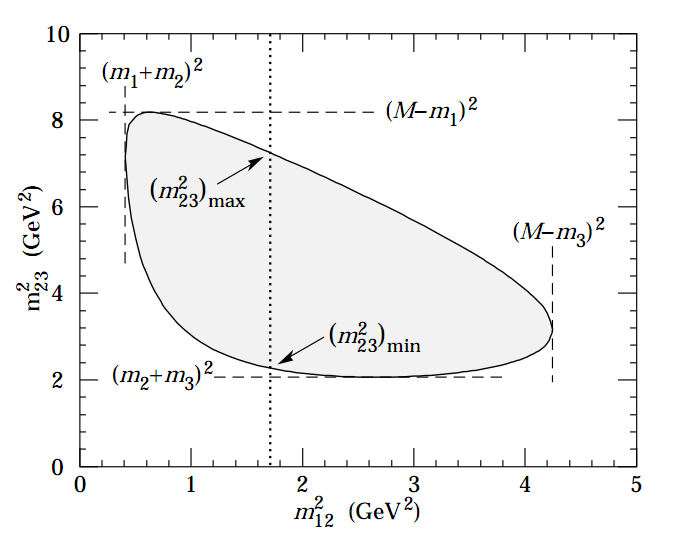
\includegraphics[width=0.5\textwidth]{immagini/Dalitz.png}
	\caption{Esempio di Dalitz Plot.}
	\label{fig:Dalitz}
\end{figure}
Adesso manca di osservare che nelle variabili scelte l'elemento infinitesimo dello spazio delle fasi di può scrivere come:
\[
	dL_p = \frac{1}{32s} \ ds_{12} \ ds_{23} \ d\alpha \ d\left( \cos(\beta) \right) \ d\gamma 
.\] 

Questo risultato mostra che lo spazio delle fasi è uniformemente popolato nella zona permessa (piatto) se si utilizzano le variabili descritte.\\

Venendo al dunque si ha che, sperimentalmente, quando questo spazio non è uniformemente popolato si può dedurre che vi sia un processo intermedio non previsto: un decadimento a due corpi in cui uno dei prodotti decade a sua volta in cue corpi, si hanno allora degli addensamenti nello spazio delle fasi in zone che ci indicano la massa invariante della particella instabile (dal decadimento a due). Questo è il metodo della massa invariante.



 % risposto 
\section{Domande b}
\subsection[]{ Calcolare la "resistenza di irraggiamento" di un circuito elettrico quadrato di lato L, piccolo rispetto alla lunghezza d'onda $\lambda$ della radiazione monocromatica incidente, se il circuito è puramente resistivo con resistenza R.\\
Calcolare anche la sezione d'urto di assorbimento e la sezione d'urto elastica se l'onda incidente ha campo magnetico perpendicolare al piano del circuito e di modulo massimo $B_0$. }
Nomi a parte il problema è schematizzato in Figura:
\begin{figure}[H]
	\centering
	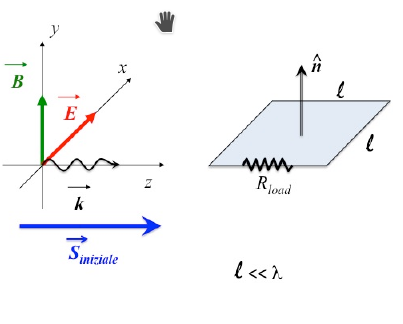
\includegraphics[width=0.5\textwidth]{immagini/spira_onda.png}
	\caption{Spira immersa nel campo di onda e.m.}
	\label{fig:spira1}
\end{figure}
\paragraph{Calcolo della resistenza di irraggiamento.}
I campi ed il vettore di Poynting dell'onda sono:
\[
	\boldsymbol{E} = E_x \hat{i} = E_0 \cos\left( \omega t - kz \right) \hat{i} 
.\] 
\[
	\boldsymbol{B} = B_y \hat{j} = B_0 \cos\left( \omega t - kz \right) \hat{j} 
.\] 
\[
	\boldsymbol{S}_{in} = \frac{E_0^2}{Z_0}\cos\left( \omega t - kz \right) \hat{k} 
.\] 
Sia $I\left( t \right) $ la corrente che scorre nel circuito; possiamo sfruttare le ipotesi di dimensioni piccole (rispetto a $\lambda$) per dire che tale corrente è uniforme in tutta la spira. Trascurando anche autoinduttanza e capacità parassite possiamo affermare che il circuito ha momento di dipolo nullo.\\
Non vale lo stesso per il momento di dipolo magnetico:
\[
	\boldsymbol{p}_m = I\left( t \right) l^2 \hat{j}
.\] 
Adesso aggiungendo le ipotesi di perfetta monocromaticita dell'onda incidente e di nessuna perdita di energia per irraggiamento del circuito si calcola la corrente $I\left( t \right)$ applicando Faraday:   
\[
	\varepsilon\left( t \right) = - \frac{\mbox{d} \Phi\left( \boldsymbol{B} \right) }{\mbox{d} t} = R_{load} I\left( t \right) 
.\]
Mettiamo quindi in mezzo la geometria del circuito:
\[
	I\left( t \right) = \frac{\varepsilon\left( t \right)}{R_{load}} = 
	- \frac{1}{R_{load}} \frac{\mbox{d} \Phi\left( \boldsymbol{B} \right) }{\mbox{d} t} 
	= - \frac{1}{R_{load}} \frac{\mbox{d}}{\mbox{d}t} \left[ \int_{-l/2}^{l/2} B_0 \cos\left( \omega t - kz \right) l dz \right] 
	= \frac{\omega l^2B_0\sin\left( \omega t\right)}{R_{load}} \frac{\sin\left( kl/2 \right)}{kl/2}      
.\] 
Agginungendo l'approssimazione:
\[
	\frac{kl}{2} = \frac{\pi l}{\lambda} \ll 1 \implies I\left( t \right) = \frac{\omega l^2 B_0 \sin\left( \omega t \right) }{R_{load}}  
.\] 
Possiamo allora calcolare la potenza irraggiata:
\[
	P_{el} = \frac{\left| \ddot{\boldsymbol{p_m}} \right| ^2}{6\pi \epsilon_0 c^{5}} = \frac{\ddot{I}^2\left( t \right) l^4}{6\pi \epsilon_0 c^5}
.\] 
Se si effettua un bilancio energetico del circuito:
\[
	\varepsilon I = R_{load}I^2 + P_{el} = R_{load} I^2 + \frac{l^4}{6\pi \epsilon_0 c^5}\ddot{I}^2
.\] 
Nel caso in analisi la f.e.m. è armonica 
\[
	\varepsilon = \varepsilon_0 \sin\left( \omega t \right) \quad 
	\text{ con } \quad  
	\varepsilon_0 = \omega l^2 B_0
\]
Quindi la soluzione stazionaria per la corrente sarà anch'essa armonica: $I = I_0 \sin\left( \omega t \right) $, in conclusione:
\[
	\varepsilon I = R_{load}I^2 + \frac{\omega ^{4}l^{4}}{6\pi \epsilon_0 c^{5}} \implies \varepsilon = \left( R_{load} + R_{irr} \right) I
.\] 
Dove è stata definita la resistenza di irraggiamento (dipendente dalla frequenza):
\[
	R_{irr} = \frac{\omega^4l^4}{6\pi \epsilon_0 c^5}
.\]
Espressa in funzione della lunghezza d'onda:
\[
	R_{irr} = \omega^4 \frac{l^4}{6\pi \epsilon c^5} = \left( \frac{2\pi c}{\lambda} \right) ^4 \frac{l^4\sqrt{\mu_0 \epsilon_0} }{6 \pi \epsilon_0 c^4} = \frac{8}{3}\pi^3 Z_0\left( \frac{l}{\lambda} \right)^4 = 31.1 \text{ k}\Omega \left( \frac{l}{\lambda} \right)^4  
.\] 
\paragraph{Calcolo delle sezioni d'urto.}
Notando che 
\[
	I\left( t \right) = \frac{\varepsilon\left( t \right) }{\left( R_{load} + R_{irr} \right) }
.\] 
Possiamo ottenere la potenza assorbita e la potenza "elastica":
\[
	P_{abs} = R_{load} I^2 = \frac{R_{load}}{\left( R_{load} + R_{irr} \right) ^2}\varepsilon^2
.\] 
\[
P_{el} = R_{irr} I^2 =  \frac{R_{load}}{\left( R_{load} + R_{irr} \right) ^2}\varepsilon^2
.\] 
Quindi la potenza trasferita al carico è massima per $R_{load} = R_{irr}$.\\
Adesso basta mediare il vettore di Poynting per concludere:
\[
\left< \left| \boldsymbol{S}_{in} \right| \right> = \frac{\boldsymbol{E}_0^2}{2Z_0}
.\] 
llora le sezioni d'urto sono:
\[
	\sigma_{abs} = \frac{4\pi^2}{\lambda^2}l^4Z_0 \frac{R_{load}}{\left(R_{load} + R_{irr}\right)^2}
.\] 
\[
	\sigma_{irr} = \frac{4\pi^2}{\lambda^2}l^4Z_0 \frac{R_{irr}}{\left(R_{load} + R_{irr}\right)^2}
.\]
\[
	\sigma_{tot} = \sigma_{irr} + \sigma_{load} = \frac{4\pi^2}{\lambda^2}l^4Z_0 \frac{Z_0}{\left(R_{load} + R_{irr}\right)^2}
.\] 

\subsection[]{ Utilizzando le apposite tabelle che forniscono le masse dei nuclei, determinare il Q-valore o l'energia di soglia dei seguenti processi, valutando l'eventuale ruolo della interazione coulombiana nello stato iniziale:
\begin{enumerate}	
	\item	p + 40Ar $\implies$ p + 39Ar + n 
	\item	p + 14N $\implies$ X + n
	\item	p + 16O $\implies$ X + n
	\item	n + 14N $\implies$ 14C + p
	\item	4He + 14N $\implies$ 17O + p
	\item	2H + 3H $\implies$ 4He + n
	\item	2H + 2H $\implies$ 4He + $\gamma$
	\item	p + 198Hg $\implies$ 197Au + p + p
\end{enumerate}
}
Partiamo con un pò di teoria:
\[
	Q = \sum M_{in} - \sum M_{fin} 
.\] 
Se il Q-valore è positivo allora la reazione avviene in modo spontaneo: l'energia di soglia è nulla.\\
Se il Q-valore è negativo allora l'energia di soglia è maggiore di zero e dipende dalla carica del proiettile.
Se la particella proiettile è neutra allora l'energia di soglia è il modulo del Q-valore, altrimenti è necessario calcolare l'energia necessaria a vincere l'interazione columbiana per arrivare al nucleo (essendo le interazioni sopra scritte tutte forti) nel sistema del laboratorio.\\
Per effettuare il calcolo sfruttiamo la conservazione dell'energia e della quantità di moto non relativistiche in una dimensione, chiariamo la notazione:
\begin{itemize}
	\item $R$: raggio del nucleo colpito 
	\item $m_{prt}$: massa del proiettile.
	\item v$_0$: velocità iniziale del proiettile.
	\item $T$: energia cinetica iniziale del proiettile.
	\item $Z$: protoni del nucleo colpito.
	\item  $M$: massa del nucleo colpito.
	\item $d$: distanza in cui i nuclei si urtano definita dalla somma dei raggi delle due particelle coinvolte:
		 \[
			 d = R + r_{prt} \approx \left( 1.25 A^{1/3} + r_{\text{skin}} + r_{prt} \right) \text{ fm} = \left( 1.25 A^{1/3} + 2 + r_{prt} \right) \text{ fm}  
		.\] 
\end{itemize}
Facendo il conto:
 \[
\begin{cases}
	m_{prt}\text{v}_0 = \left( m_p + M \right)V_{cm}\\
	T \ge \frac{1}{2}\left( m_{prt} + M \right)V_{cm} + \frac{Ze^2}{4\pi \epsilon_0 d} \\
	T = \frac{1}{2}m_{\text{prt}}\text{v}_0^2
\end{cases}
\]
Quindi sviluppando per $T$ si ottinene l'energia cinetica necessaria per la reazione:
\[
	T \ge \left( 1 + \frac{m_{prt}}{M} \right) \frac{Ze^2}{4\pi \epsilon_0 d} = T_{\text{min}} 
.\] 
e per l'energia di soglia dobbiamo soltanto sommare il modulo del Q-valore:
\[
	E_{\text{soglia}} = T_{\text{min}} + \left| Q \right| 
.\] 
In questo modo possiamo risolvere tutte le interazioni elencate.

\paragraph{Interazione 1.}
Bisogna notare che $40 \text{Ar} = \ce{^{40}_{18}\text{Ar}}$ (vedi tabelle con difetti di massa), quindi:
\[
	\ce{p + 40\text{Ar} -> p + 39\text{Ar} + n}
.\] 
\[
	Q = \left( m_p + 40m_u + \Delta_{40, 18} \right) - \left( m_p + 39 m_u + \Delta_{39, 18} + m_n  \right) = m_u + \Delta_{40, 18} - \Delta_{39, 18} - m_n      
.\]
Numericamente:
\[
	Q \approx \left( 931.49 + \left( -35.04 \right) - \left( -33.24 + 939.57 \right)  \right)\text{Mev} \approx -8.3 \text{ MeV} \quad \quad \text{Reazione endotermica}
.\]
Per il calcolo dell'energia di soglia applichiamo subito quando visto sopra:
\[
	E_{\text{soglia}} = \left( 1 + \frac{m_p}{M_{40\text{Ar}}} \right) \frac{Ze^2}{4 \pi \epsilon_0 d} + \left| Q \right| \quad \quad 
	\text{con } M_{40Ar} = 40m_u + \Delta_{40,18}
.\]
si calcola la distanza minima d (il raggio del protone è circa 1.25 fm): 
\[
	d \approx \left( 1.25 \cdot \left( 40 \right)^{ 1/3 } + 2 + r_{protone} \right)\text{fm} \approx 6.25 \text{ fm} 
.\] 
Quindi l'energia di soglia (calcolo numerico approssimato a mente\ldots):
\[
	E_{\text{soglia}} \approx 4 \text{ MeV} + 8 \text{ MeV} \approx 12 \text{ MeV}   
.\] 
Analogamente per le altre reazioni.

\subsection[]{  Dimostrare la relazione fra la definizione della sezione d’urto elastica nel caso di fotoni incidenti su un unico bersaglio e la definizione di sezione d'urto elastica per un’onda e.m. monocromatica su un unico bersaglio.}
Nel caso di onda monocromatica su un bersaglio si ha:
\[
	\sigma_{\text{el}} = \frac{\left< P_{el}\right>}{\left<\left| \boldsymbol{S}_{in} \right|  \right>}
.\]
Mentre per un fascio di fotoni incidenti:
\[
	\sigma_{\text{el}} = \frac{\frac{\mbox{d} N_{el}}{\mbox{d} t}}{\left| \boldsymbol{j}_{\gamma}\right|}
.\] 
L'equivalenza delle due deriva dal fatto che se si moltiplica e si divide la seconda per $ \hbar \omega$:
\[
	\sigma_{\text{el}} = \frac{\frac{\mbox{d} N_{el}}{\mbox{d} t}}{\left| \boldsymbol{j}_{\gamma}\right|} = \frac{\frac{\mbox{d} N_{el}}{\mbox{d} t}\hbar \omega }{\left| \boldsymbol{j}_{\gamma}\right|\hbar \omega} = \frac{\left< P_{el}\right>}{\left<\left| \boldsymbol{S}_{in} \right|  \right>}
.\] 	

\subsection[]{  Quale calcolo si deve effettuare per determinare il numero di eventi per unità di tempo e di volume che si producono negli urti fra particelle di due specie diverse e differenti concentrazioni le cui velocità relative sono distribuite con un funzione $f(V_{rel})$, normalizzata all'unità, e la cui sezione d'urto è $\sigma(V_{rel})$?}
Date due specie con densità volumica $n_a$ e  $n_b$ che si scontrano e con densità di prodotti $n_f$, se la $ f\left( V_{\text{rel}} \right) $ è normalizzata allora si ha:
\[
	\frac{\mbox{d} n_{\text{f}}}{\mbox{d} t } = n_a n_b \int_0^{\infty} f\left( v_{rel} \right) \sigma_{\text{f}}\left( v_{rel} \right) v_{rel} dv_{rel}
.\] 
Tipicamente la $f\left( V_{rel} \right)$ è gaussiana. 

\subsection[]{ Calcolare l'attenuazione di un fascio di particelle incidenti su un materiale omogeneo e composto da atomi di una sola specie in funzione della profondità [dati: sezione d'urto del processo su ogni atomo del bersaglio, densità di massa del mezzo, numero atomico del mezzo].}
\label{sec:2.b.5}
\paragraph{Lamina sottile}
Data una lastra di materiale omogeneo definiamo alcune (tante, forse troppe) quantità utili: spessore $\Delta x$, densità $\rho$, area $\Delta S$, volume di lastra considerato $V$ , sezione d'urto su ogni atomo bersaglio (totale) $ \sigma_{\text{tot}}$, $n_b$ la concentrazione di besagli nel materiale e $n_a$ la concentrazione di particelle incidenti. Possiamo riscrivere queste in funzione delle quantità date dal testo e sfruttare qualche utile relazione.\\ 
Partiamo da $n_b$: definendo $M_{\text{tot}}$ la massa totale di lastra nel volume, $M_A$ la massa di una mole della sostanza del materiale in grammi, $N_a$ il numero di avogadro si ha:
\[
	V \cdot n_b = N_{\text{tot}} = \frac{M_{\text{tot}}}{M_A} N_a \implies n_b =\frac{N_{\text{tot}}}{V} = \frac{\rho}{M_A} N_a
.\]
La probabilità di interazione nel volume considerato è definita da:
\[
	P_{\text{int}} = n_b \cdot \sigma_{\text{tot}} \Delta x  = \frac{\rho N_a }{M_A} \sigma_{\text{tot}}\Delta x
.\] 
A questo punto si vede come è definita la profondità di penetrazione (essendo la $P_{\text{int}}$ adimensionale):
\[
	\mathcal{L} = \frac{M_A}{\rho N_a\sigma_{\text{tot}}}
.\] 
quindi l'attenuazione è data dalla frazione di particelle che riescono a passare, quantità che si può ricavare come il complementare della probabilità di interagire: la probabilità di passare.
\[
	A = 1 - \frac{\Delta x}{\mathcal{L}} \quad \quad 
	\text{Nel caso di lamina sottile}
.\] 
Quanto visto fin'ora funziona finche la lamina si può considerare sottile: $\Delta x < \mathcal{L}$, se questa approssimazione viene meno è necessario rivedere alcuni conti.
\paragraph{Materiale generico} Possiamo pensare ad un materiale generico come la sovrapposizione di tante lamine sottili di diversa superficie. Si può quindi vedere la probabilità di interazione come una funzione della posizione $P_{\text{int}}\left( x \right)$, quindi anche la stessa attenuazione sarà funzione della posizione $A\left( x \right) $. Calcoliamo l'attenuazione alla posizione $x + \Delta x$, dobbiamo utilizzare le regole delle probabilità combinate:
\[
	A\left( x + \Delta x \right) = A\left( x \right) A\left( \Delta x \right) = A\left( x \right) \left( 1- P_{\text{int}}\left( \Delta x \right)  \right) = A\left( x \right) \left( 1 - \frac{\Delta x }{\mathcal{L}} \right)  
.\]
Applicando il rapporto incrementale risulta quindi evidente che il risultato sarà esponenziale ( cosa che goffamente sapevamo già dal momento che si applicano le proprietà della probabilità di eventi ripetuti).
\[
	\frac{A_{\text{int}}\left( x + \Delta x \right) - A_{\text{int}}\left( x \right)}{\Delta x} = -\frac{A\left( x \right) }{\mathcal{L}} 
.\]
Facendo tentere $\Delta x$ a zero:
\[
	\dot{A} = -\frac{A}{\mathcal{L}} \implies A\left( x \right) = e^{-x/\mathcal{L}} \quad \quad 
	\text{Materiale generico}
.\] 

\subsection[]{  Calcolare l'attenuazione di un fascio di particelle incidenti su un materiale omogeneo e composto da atomi di diverse specie in funzione della profondità [dati: sezione d'urto del processo su ogni atomo del bersaglio, densità di massa del mezzo, numeri atomici, composizione chimica del mezzo]}
\paragraph{Lamina sottile}
Essendo nota la composizione chimica del mezzo è noto anche la percentuale di atomi che compongono il materiale:
\[
	\text{Composizione del mezzo: } \ X^{\left( 1 \right) }_{a_1}\ldots X^{(N)}_{a_N}
.\]
Con $X^{i}$ specie atomica, $a_j$ pedice che indica la composizione chimica nella formula del composto (per non appesantire si trascurano le formule con simboli ripetuti tipo $CH_3COOH$).
Si può quindi ragionare come se avessimo N copie del nostro materiale ognuno interamente composto da una singola specie preservando le densità $\rho_i$ che sono presenti nel materiale originale, successivamente si applica il principio di sovrapposizione sommando tutte le attenuazioni e normalizzando sulle N specie:
\[
	A_i = 1 - \frac{\Delta x}{\mathcal{L}_i} \implies A_{\text{tot}} = \frac{\sum_{n=1}^{N} A_n}{N} = 1 - \sum_{n=1}^{N} \frac{\Delta x}{N \mathcal{L}_n}
.\] 
con la penetrazione definita a partire dalla densità e dalla massa molare delle singole specie:
\[
	\mathcal{L}_i = \frac{M_{A}^{\left( i \right) }}{\rho_i N_a \sigma_{\text{tot}}}
.\]
\paragraph{Materiale generico}
Con passaggi del tutto analoghi alla domanda precedente si arriva alla conlcusione:
\[
	A_{\text{tot}} =\frac{\sum_{n=1}^{N} e^{-x/\mathcal{L}_n}}{N} 
.\] 
\subsection[]{  Effettuare una stima numerica della sezione d'urto totale forte per i seguenti urti: 
\begin{enumerate}
	\item	p + 40Ar
	\item	n + 14N
	\item	4He + 14N
	\item	2H + 3H
\end{enumerate}
}
Se si considera solo la sezione d'urto forte non c'è bisogno di preoccuparsi di interazioni elettrodeboli: si suppone che l'energia sia sufficiente da poter trascurare questo tipo di interazioni. Il calcolo si riduce alla stima della superficie di possibile impatto tra i due oggetti assunti come sferici:
\[
	\sigma_{\text{strong}} \approx \pi\left( R_1 + R_2 \right)^{2} 
.\] 
Con $R_1$ e  $R_2$ raggi delle particelle interagenti. Per tutti gli atomi in gioco ho scelto di considerare sempre $r_\text{skin}$.
\paragraph{Interazione 1.}
\[
	\sigma_1 \approx \pi\left( r_p + R_{40\text{Ar}} \right)^{2}  \approx \pi (1.25 \cdot (40)^{1/3} + 2 + 1.25 )^{2} \text{ fm}^{2} \approx \pi \cdot (6.25)^{2} \text{ fm}^{2}
\]
Quindi 
\[
	\sigma_1 \approx \pi \cdot 39 \text{ fm}^{2} \approx 120 \text{ fm}^{2} = 1.2 \text{b}
\]
\paragraph{Interazione 2.} 
$\sigma_2 \approx 1.23 \text{b}$

\paragraph{Interazione 3.}
$\sigma_3 \approx 2.54 \text{b} $

\paragraph{Interazione 4.}
$\sigma_4 \approx 1.7 \text{b}$

\subsection[]{  Calcolare l’energia che dovrebbe avere un protone che incide su un protone fermo per ottenere una energia nel centro di massa pari a quella di LHC (14TeV).}
Sia $E$ l'energia del protone nel laboratorio, si ha:
\[
	E^2_{\text{cm}} = \left( E_{lab} \right)^{2} -  \boldsymbol{P}_{\text{lab}}^{2} = \left( E + m_p \right)^{2} - \left(E^2 - m_p^2\right) = 2m_p^2 + 2m_pE 
.\]
Quindi l'energia necessaria è circa $E = 10^{6} $ TeV

\subsection[]{ Calcolare l'energia di degli elettroni/positroni per innescare la reazione:
\[
	e^{+} \ + \ e^{-} \implies p \ + \ \overline{p}
\] 
in cui i due leptoni collidono con 3-impulsi opposti e di modulo diverso.}

Se $E_1$ e $E_2$ sono le energie dei due leptoni si ha 
\[
	\left( E_1 + E_2 \right) ^2 - \left( \sqrt{E_1^2 - m_e^2} - \sqrt{E_2^2 - m_{e}^2}  \right) \ge 4 m_p^2
.\]
L'energia di soglia si ottinene studiando la funzione nelle due variabili sopra, da lì si evince che il minimo si ha per $E_1 = E_2$, quindi:
\[
	E_{\text{min}} = m_p
.\] 

\subsection[]{ Calcolare l’energia di soglia nel laboratorio per le seguenti reazioni (la seconda particella è inizialmente ferma):
\begin{enumerate}
	\item	$\gamma \ + \ {}^{16} O \implies e^{+} \ + \ e^{-} \ + \ {}^{16}O $
	\item	$\gamma \ + \ e^{-} \implies e^{-} \ + \ e^{+} \ + \ e^{-}$
	\item	$p \ + \ p \implies p \ + \ p \ + \ p \ + \ \overline{p}$
	\item	$p \ + \ {}^{16}O \implies p \ + \ p \ + \ \overline{p} \ + \ {}^{16}O$
	\item	$e^{+} \ + \ e^{-} \implies p \ + \ \overline{p}$
	\item	$e^{-} \ + \ p \implies n \ + \ \nu_e$
	\item	$\overline{\nu_e} \ + \ p  \implies n \ + \ e^{+}$
\end{enumerate}
}

Per tali calcoli è necessaria una generalizzazione della risposta al quesito precedente, è infatti richiesto che:
\[
	\left( \sum_i P_{i,\text{in}} \right)^2 \ge \left(\sum_{i} m_{i, \text{fin}} \right)^2  
.\] 
Adesso si può sfruttare il fatto che i reagenti sono soltanto due e che il secondo è sempre a riposo (generalizzazione della domanda 2.b.8):
\[
	E_1 \ge \frac{1}{2m_2}\left[ \left( \sum_{i} m_{i, \text{fin}} \right)^2 - \left( m_1^2 + m_2^2 \right)  \right] 
.\]
E adesso si tratta solo di infilare dentro i numeri.

\subsection[]{ Calcolare la probabilità che un neutrino interagisca nell’attraversare la Terra lungo un diametro.\\
Nota: sia assuma che l’energia del neutrino sia tale che la sezione d’urto totale su un singolo nucleone sia 1 fb. } 
Si assume per il calcolo $\rho_{\text{T}} \approx 5.5 \text{g}/\text{cm}^3$.\\
Possiamo ipotizzare una bassa probabilità di interazione per il neutrino, è quindi possibile assumere la terra come una lamina sottile (con immenso piacere dei terrapiattisti) e calcolare la probabilità cercata come:
\[
P_{\text{int}} = n \sigma d \approx 4.2 \cdot 10^{-5} 
.\] 
Con $d \approx 12.76 \cdot 10^{3} \text{ km}$ raggio terrestre e $n \approx \rho_{\text{T}}\cdot N_A\cdot A / M_{\text{Si}} = \rho\cdot N_{\text{A}} / 1 \text{[g]} \approx 5.5\cdot 6 \cdot 10^{23} \text{cm}^{-3}$ densità media della terra (composta principalmente da Silicio).

\subsection[]{ Dimostrare che un elettrone (non relativistico) soggetto ad una forza elastica di richiamo, ad una forza di attrito viscoso ed alla forza di reazione radiativa, nel campo di un’onda e.m. piana polarizzata linearmente oscilla con la legge:
\[
	\boldsymbol{x} = \frac{e \boldsymbol{E_0}}{m_{e}} \frac{1}{\omega_0^2-\omega^2-i\omega\Gamma_{tot}} e^{-i \omega t} \quad \quad 
	\text{ con }  \quad \quad
	\Gamma_{tot} = \Gamma' + \Gamma \frac{\omega^2}{\omega_{0}^2}
\] 
} \label{subsec: 2.b.12}
Facendo riferimento ai risultati delle Domande \hyperref[subsec: 2.a.15]{2.a.15}, \hyperref[subsec: 2.a.16]{2.a.16}  si prosegue con il calcolo.
L'equazione di moto dell'elettrone in questo caso è (considerando anche la $F_{\text{rad}}$):
\[
m_e \ddot{\boldsymbol{x}} = q \boldsymbol{E_0}e^{-i \omega t} - m_e \tau \dddot{\boldsymbol{x}} - m_e \Gamma' \dot{\boldsymbol{x}}
.\] 
Spostando l'incognita vettoriale a destra si ha:
\[
-\tau \dddot{\boldsymbol{x}} + \ddot{\boldsymbol{x}} + \Gamma' \dot{\boldsymbol{x}} + \omega _0^2 \boldsymbol{x} = \frac{q \boldsymbol{E_0}}{m_e} e^{-i \omega t}
.\] 
Cercando la soluzione stazionaria $\boldsymbol{x} = \boldsymbol{x}_0 e^{-i \omega t}$ si ha:
\[
	-\tau \left( -i \omega \right)^3 \boldsymbol{x}_0e^{-i \omega t} + \left( - i \omega \right) \Gamma'\boldsymbol{x}_0 e^{-i \omega t} + \omega _0^2 \boldsymbol{x}_0 e^{-i \omega t} = \frac{q \boldsymbol{E}_0}{m_e} e^{-i \omega t}
.\] 
Quindi:
\[
\boldsymbol{x}_0 = \frac{q \boldsymbol{E}_0/m_e}{ \omega _0^2 - \omega ^2 -i \omega \Gamma' - i \tau \omega ^2 }
.\]
È quindi utile definire $\Gamma_{\text{tot}} = \Gamma' + \tau \omega ^2 = \Gamma' + \Gamma \frac{\omega ^2}{\omega _0^2}$ per giungere alla conclusione:
\[
\boldsymbol{x} = \frac{q \boldsymbol{E}_0}{m_e} \frac{e^{-i \omega t}}{\omega _0^2 - \omega ^2 - i \omega \Gamma_{\text{tot}}} 
.\] 

\subsection[]{Dimostrare che la sezione d’urto differenziale elastica per un’onda e.m. piana e monocromatica su un elettrone legato elasticamente vale 
\[
	\frac{\mbox{d} \sigma_{el}}{\mbox{d} \Omega} = r_e^2 L\left( \omega \right) \sin^2\left( \alpha  \right)    
\]
con $\alpha$ angolo fra la direzione di osservazione e direzione di polarizzazione (lineare) dell'onda.} \label{subsec: 2.b.13}
La risposta al quesito è stata prematuramente scritta alla Domanda \hyperref[subsec: 2.a.16]{2.a.16} facendo uso del risultato ottenuto nella Domanda \ref{subsec: 2.b.12}.
Si riaccenna solo al fatto che è stata definita $L\left( \omega  \right)$ come:
\[ 
	L \left( \omega \right) = \frac{\omega^4}{\left( \omega_{0}^2 - \omega^2 \right)^2 + \omega^2 \Gamma_{tot} } \quad \quad 
.\] 
Vediamo di dimostrare quanto scritto, sopra abbiamo ottenuto:
\[
\boldsymbol{x} = \frac{q \boldsymbol{E}_0}{m_e} \frac{e^{-i \omega t}}{\omega _0^2 - \omega ^2 - i \omega \Gamma_{\text{tot}}} 
.\] 
Calcoliamo il vettore di Poynting (mediato nel tempo) associato alla potenza irraggiata dall'elettrone:
Esplicitando l'espressione del .. in funzione della variabile $\alpha$ del problema si ha:
\[
	\boldsymbol{E_{\text{dip}}} =k_0 \frac{\left( e\ddot{\boldsymbol{x}} \wedge \hat{r}\right) \wedge \hat{r}}{\left| \boldsymbol{r} \right| c^2} 
.\] 
\[
	\left<\boldsymbol{S}_{\text{el}} \right> = \left< \boldsymbol{E} \wedge H\right> = \left<\frac{\left| \boldsymbol{E}_{\text{dip}} \right|^2}{c \mu_0}  \right> = 
	k_0^2\frac{\left| e \ddot{\boldsymbol{x}}  \right|^2 \sin^2\left( \alpha  \right) }{c^4 r^2 \mu_0 } =
	\frac{1}{32 \pi^2 \epsilon_0} \frac{ \left| e \ddot{\boldsymbol{x}}_0 \right|^2 \sin^2\left( \alpha \right) }{c^3 r^2} \hat{r}
.\] 
Che in CGS risulta più elegante:
\[
\left<\boldsymbol{S}_{\text{el}} \right> = \frac{1}{8 \pi} \frac{ \left| e \ddot{\boldsymbol{x}}_0 \right|^2 \sin^2\left( \alpha \right) }{c^3 r^2} \hat{r} 
.\] 
Dividendo questo vettore per il vettore di poynting iniziale (da qui in poi CGS per semplicità) si ottiene l'espressione cercata:
\begin{align*}
\frac{\mbox{d} \sigma_{\text{el}}}{\mbox{d} \Omega} = \frac{\left< \boldsymbol{S}_{\text{el}} \right> \cdot r^2 \hat{r}}{\frac{c}{8 \pi}\left| E_0 \right|^2 } = 
\frac{ \omega^{4} e^{4}}{c^{4}m_e^2} \frac{\sin^2\left( \alpha  \right) }{\left( \omega _0^2 - \omega ^2 \right)^2 + \omega ^2 \Gamma_{\text{tot}}^2} =
r_e^2 \frac{\omega ^{4}\sin^2\left( \alpha \right)}{\left( \omega _0^2 - \omega ^2 \right)^2 + \omega ^2 \Gamma_{\text{tot}}^2}
.\end{align*}
Dove è necessario riconoscere il raggio classico in CGS:
\[
	r_e^{\left( \text{CGS} \right) } = \frac{e^2}{c^2m_e}
.\] 
Va da se che in MKSA:
\[
	\frac{\mbox{d} \sigma_{\text{el}}}{\mbox{d} \Omega} = \left( \frac{k_0 e^2}{m_e c^2} \right) ^2 \frac{\omega ^{4}\sin^2\left( \alpha \right)}{\left( \omega _0^2 - \omega ^2 \right)^2 + \omega ^2 \Gamma_{\text{tot}}^2}
.\] 

%2.b.14
\subsection[]{Dimostrare che la sezione d’urto Thomson vale $\sigma_{Th} = \frac{8}{3}\pi r_{e}^2  = 0.66 \text{ barn}$.}
Si può arrivare allo Scattering Thompson riscrivendo l'equazione di moto dell'elettrone e trascurando la pressione di radiazione di cui si è invece fatto uso nelle precedenti domande:
\[
m_e \ddot{\boldsymbol{x}}= e \boldsymbol{E}_0 e^{-i \omega t}
.\] 
La potenza irraggiata di dipolo sarà quindi:
\[
P_{\text{irr}} = k_0 \frac{e^2 \left| \ddot{\boldsymbol{x}} \right|^2}{3c^3} 
.\]
Sviluppando i conti e ricordando la definizione di sezione d'urto si arriva banalmente a:
\[
\sigma_{\text{Th}}=\frac{8}{3}\pi r_e^2
.\] 
Ricordando ancora che il \hyperref[eq: raggio classico]{Raggio classico dell'elettrone} è: $r_e = k_0 \frac{e^2}{m_e c^2} \approx 2.82$ fm.

%2.b.15
\subsection[]{Dimostrare che la sezione d’urto elastica per un’onda e.m. piana e monocromatica su un elettrone legato elasticamente vale:
\[
	\sigma_{el} = \sigma_{Th} L\left( \omega \right) 
\] 
}
È in pratica richiesto di trovare la Funzione di Brieght-Wiegner. Visto che abbiamo la sezione differenziale tuttavia è sufficiente integrarla su tutti gli angoli. Ci si riduce allora al calcolo dell'integrale:
\[
	\int \sin^2\left( \alpha  \right) d \Omega = \int \frac{1 + \cos^2\left( \alpha \right) }{2} d\Omega = 2\pi + \frac{1}{2} 2 \pi \int_0^{2\pi} \cos^2\left( \alpha  \right) \sin\left( \alpha  \right) d \alpha = \frac{8}{3}\pi  
.\] 
Tutto il resto esce indisturbato dall'integrale sull'angolo solido, da cui la tesi.

%2.b.16
\subsection[]{Dimostrare che la sezione d’urto totale per un’onda e.m. piana e monocromatica su un elettrone legato elasticamente vale:
\[
		\sigma_{\text{tot}} = 4 \pi r_{e} c L\left( \omega \right)
\] 
}
Abbiamo gia risolto l'equazione del moto:
\[
\boldsymbol{x}= \frac{e \boldsymbol{E}_0}{m} \frac{e^{- i \omega t}}{\omega _0^2 - \omega ^2 - i \omega \Gamma_{\text{tot}}}
.\] 
Si tratta quindi solo di ricordare che la potenza totale dissipata può essere espressa come:
\[
	P_{\text{tot}} = \left<\boldsymbol{v} \cdot \boldsymbol{F} \right> = \left<\dot{\boldsymbol{x}}\cdot q \boldsymbol{E} \right> = \left< e \dot{\boldsymbol{x}} \cdot \boldsymbol{E} \right> = \frac{1}{2} q \mathcal{R}e \left\{ \dot{\boldsymbol{x}} \cdot \boldsymbol{E}^* \right\} 
.\]
Quindi:
\[
	P_{\text{tot}} = \frac{q^2 \omega ^2 \left| \boldsymbol{E}_0 \right|^2 \Gamma_{\text{tot}}}{2m\left( \left(\omega _0^2 - \omega ^2 \right) ^2 + \omega ^2 \Gamma_{\text{tot}}^2  \right) }
.\] 
Resta adesso da dividere per il vettore di Poynting incidente:
\[
\sigma_{\text{tot}} = \frac{P_{\text{tot}}}{\left<\left| \boldsymbol{S}_{\text{in}} \right|\right>} = 4 \pi r_{e} c L\left( \omega \right) 
.\] 
Per completezza si scrive anche:
\[
\sigma_{\text{abs}} = \sigma_{\text{tot}} - \sigma_{\text{el}} = 4 \pi r_{e} \omega^2 L\left( \omega \right) \left[ e \Gamma_{\text{tot}} - \frac{2}{3}r_e \omega^2 \right]
.\] 
\begin{figure}[H]
	\centering
	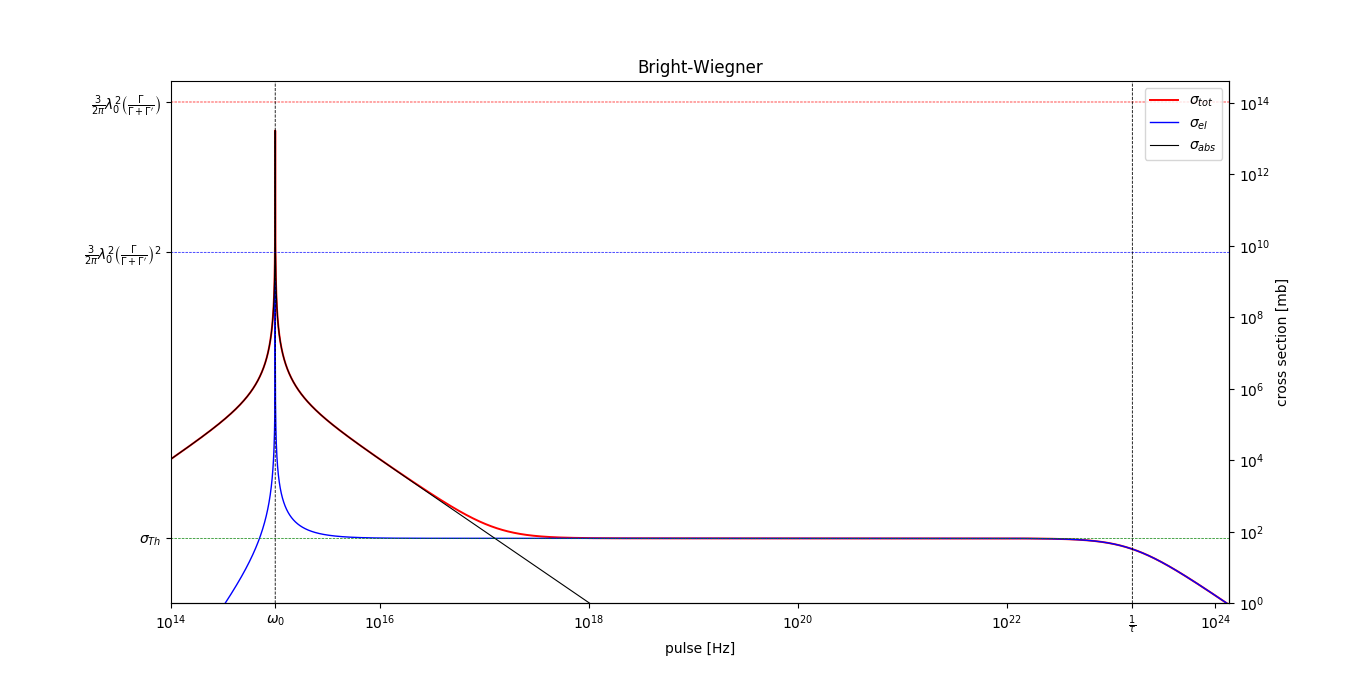
\includegraphics[width=1.1\textwidth]{immagini/b-w.png}
	\caption{Andamento delle sezioni d'urto della Bright-Wiegner}
	\label{fig:Andamento Bright-Wiegner}
\end{figure}
Nella figura si mostra come vanno le sezioni d'urto, è necessario notare che, per un rendering più fedele, sarebbero serviti più punti plottati (la funzione non ha raggiunto il massimo atteso). Per pigrizia è stato testato che arrivasse al massimo ma non è stata riportata l'immagine; insomma fidarsi o provare per credere.

%2.b.17
\subsection[]{Dimostrare che la sezione d’urto elastica per un’onda e.m. piana e monocromatica su un elettrone legato elasticamente in prossimità di una risonanza stretta (specificare il criterio) si può approssimare con una curva lorentziana
\[
	\sigma_{el} = \sigma_{Th} \frac{\omega_{0}^2 / 4}{ \left( \omega_0 - \omega \right)^2 + \frac{ \left( \Gamma' + \Gamma  \right)^2 }{4} }
\] 
}
La B-W si approssima con una lorenziana in un intorno (dell'ordine della larghezza $\Gamma + \Gamma'$) di $\omega_0$: $\omega \approx \omega_0$.\\
La risonanza è stretta se la larghezza a metà altezza è molto inferiore alla frequenza di risonanza: $\Gamma + \Gamma' \ll \omega_0$.
Passiamo alle approssimazioni allora:
\begin{align*}
	\sigma_{\text{el}} = \sigma_{\text{Th}}\frac{\omega ^{4}}{\left( \omega _0 - \omega\right)^2 \left( \omega_0 + \omega \right)^2 + \omega^2\left( \Gamma + \Gamma' \frac{\omega^2}{\omega_0^2} \right)^2} \approx \\
	\approx \sigma_{\text{Th}} \frac{\omega _0^4}{4 \omega _0^2 \left( \omega _0 - \omega  \right)^2 + \left( \Gamma + \Gamma' \right)^2 \omega _0^2  } \approx \\
	\approx \sigma_{\text{Th}}\frac{\omega_0^2/4}{\left( \omega - \omega_0 \right)^2 + \left(\frac{\Gamma + \Gamma'}{2}\right)^2 }
.\end{align*}

% 2.b.18
\subsection[]{Dimostrare che per un’onda e.m. piana e monocromatica su un elettrone legato elasticamente le sezioni d'urto al picco valgono:
\[
	\sigma_{el} = \frac{3 \lambda_{0}^2}{2 \pi} \left( \frac{\Gamma}{\Gamma + \Gamma'} \right)^2 \quad \quad \quad \quad \quad \quad \text{ }
\]
\[
	\sigma_{TOT} = \frac{3 \lambda_{0}^2}{2 \pi} \frac{\Gamma}{\Gamma + \Gamma'} \quad \quad \text{Con $\lambda_{0} = \frac{2 \pi c}{\omega_{0}}$}
\]
\[
	\sigma_{inel} = \frac{3 \lambda_{0}^2}{2 \pi} \frac{\Gamma \Gamma'}{\left( \Gamma + \Gamma' \right)^2 } \quad \quad \quad \quad \quad \quad \text{ } 
\]
}
Accettanto il fatto che tutte le tre sezioni d'urto hanno un massimo per $\omega = \omega_0$ basta prendere le sezioni d'urto e sbatterci dentro $\omega = \omega_0$.

%2.b.19
\subsection[]{Dimostrare che un elettrone (moto non relativistico) soggetto ad una forza elastica di richiamo, ad una forza di attrito viscoso ed alla forza di reazione radiativa, se viene lasciato libero di oscillare da una posizione iniziale perde energia con una 1 legge esponenziale in cui la costante tempo vale $\frac{1}{\Gamma' + \Gamma}$. Come si chiama questa costante tempo? Quale sarebbe la costante tempo con cui, invece, si smorza l'ampiezza delle oscillazioni?}
Riprendiamo l'equazione di moto dell'elettrone, tuttavia adesso togliamo la forzante dovuta all'onda incidente.
\[
	- \tau \dddot{\boldsymbol{x}} + \ddot{\boldsymbol{x}} + \Gamma' \dot{\boldsymbol{x}} + \omega_0^2 \boldsymbol{x} = 0 
.\]  
Adesso è necessario ricordare le relazioni tra i vari parametri in gioco:
\[
	\Gamma' \ll \omega_0 \ll \frac{1}{\tau}, \quad \quad \quad  
	\Gamma \ll \omega_0
.\] 
La prima è una questione puramente di grandezze fisicamente tipiche, la seconda deriva dalla prima $\left( \omega_0 \tau \ll 1 \right) $ e dal fatto che $\Gamma = \tau \omega_0^2 \ll 1 \cdot \omega_0$.\\
È quindi ragionevole cercare una soluzione oscillante e smorzante con smorzamento debole rispetto alla pulsazione:
\[
	\boldsymbol{x} = \boldsymbol{x}_0 e^{-i\left( \omega_0 - i \gamma/2 \right)t } = \boldsymbol{x}_0 e^{-i \omega_0t} e^{-\gamma t /2}, \quad \quad \quad 
	\gamma \ll \omega_0
.\]
Adesso la festa è nel sostituire questa soluzione nella equazione buttando via i termini trascurabili:
\[
	- \tau \left( -i\left( \omega_0 - i \gamma /2 \right)  \right)^3 + \left( -i\left( \omega_0 - i \gamma /2 \right) \right)^2 - \left( -i\left( \omega_0 - i \gamma /2 \right) \right) \Gamma' - \omega_0^2 = 0 
.\]
Sostituendo $\tau = \Gamma / \omega_0^2$:
\[
	-i \frac{\Gamma}{\omega_0^2}\left( \omega_0^3 - \frac{3}{2} i \gamma \omega_0^2 + \ldots \right) - \left( \omega_0^2 - i \gamma \omega_0 + \ldots \right) + 
	\left( -i \Gamma' \omega_0 - \frac{1}{2} \gamma \Gamma'  \right) + \omega_0^2 \approx 0 
.\] 
Sempre sulla base delle approssimazioni sopra è possibile notare che i termini reali sono trascurabili (raggruppare alcuni $\Gamma$ o $\Gamma'$ nei punti giusti per vederlo), ci si riduce alla forma:
\[
	-i \Gamma \omega_0 - \frac{3}{2} \Gamma \gamma - i \Gamma' \omega_0 + i \gamma \omega_0 - \frac{1}{2} \gamma \Gamma' \approx 0 \implies 
	- \Gamma \omega_0 - \Gamma' \omega_0 + \gamma \omega_0 \approx 0 
.\] 
Che ci porta alla conclusione:
\[
\gamma \approx \Gamma + \Gamma 
.\]
Quindi l'ampiezza delle oscilazioni è smorzata con una costante tempo data da:
\[
	\boldsymbol{x} = \ldots \cdot e^{- t /\tau_{\text{osc}}} \quad \quad \text{con} \quad \quad
\tau_{osc} = \frac{2}{\gamma} = \frac{2}{\Gamma + \Gamma'}
.\]
Se consideriamo invece l'andamento della energia è necessario tener conto del fatto che essa è quadratica nella velocità (cinetica) e nella posizione (potenziale): 
\[
E = E_0 e^{- \gamma t} \quad \implies \quad \tau_{\text{energia}} = \frac{1}{\gamma} = \frac{1}{\Gamma + \Gamma'}
.\]
In tutto questo macello il risultato importante è uno: la larghezza totale di uno stato risonante è il reciproco della sua vita media, risonanza stretta = particella longeva e viceversa.

% 2.b.20
\subsection[]{Calcolare la relazione tra parametro d'impatto (b) e angolo di scattering ($\theta$) nel caso di scattering di Rutherford (Coulombiano) e di scattering su sfera rigida.} 
\label{sec:2.b.20}
Prima di iniziare con questi argomenti è bene dare una rilucidatà ad alcune grandezze tipiche in esame: le dimensioni atomiche.
\begin{figure}[H]
	\centering
	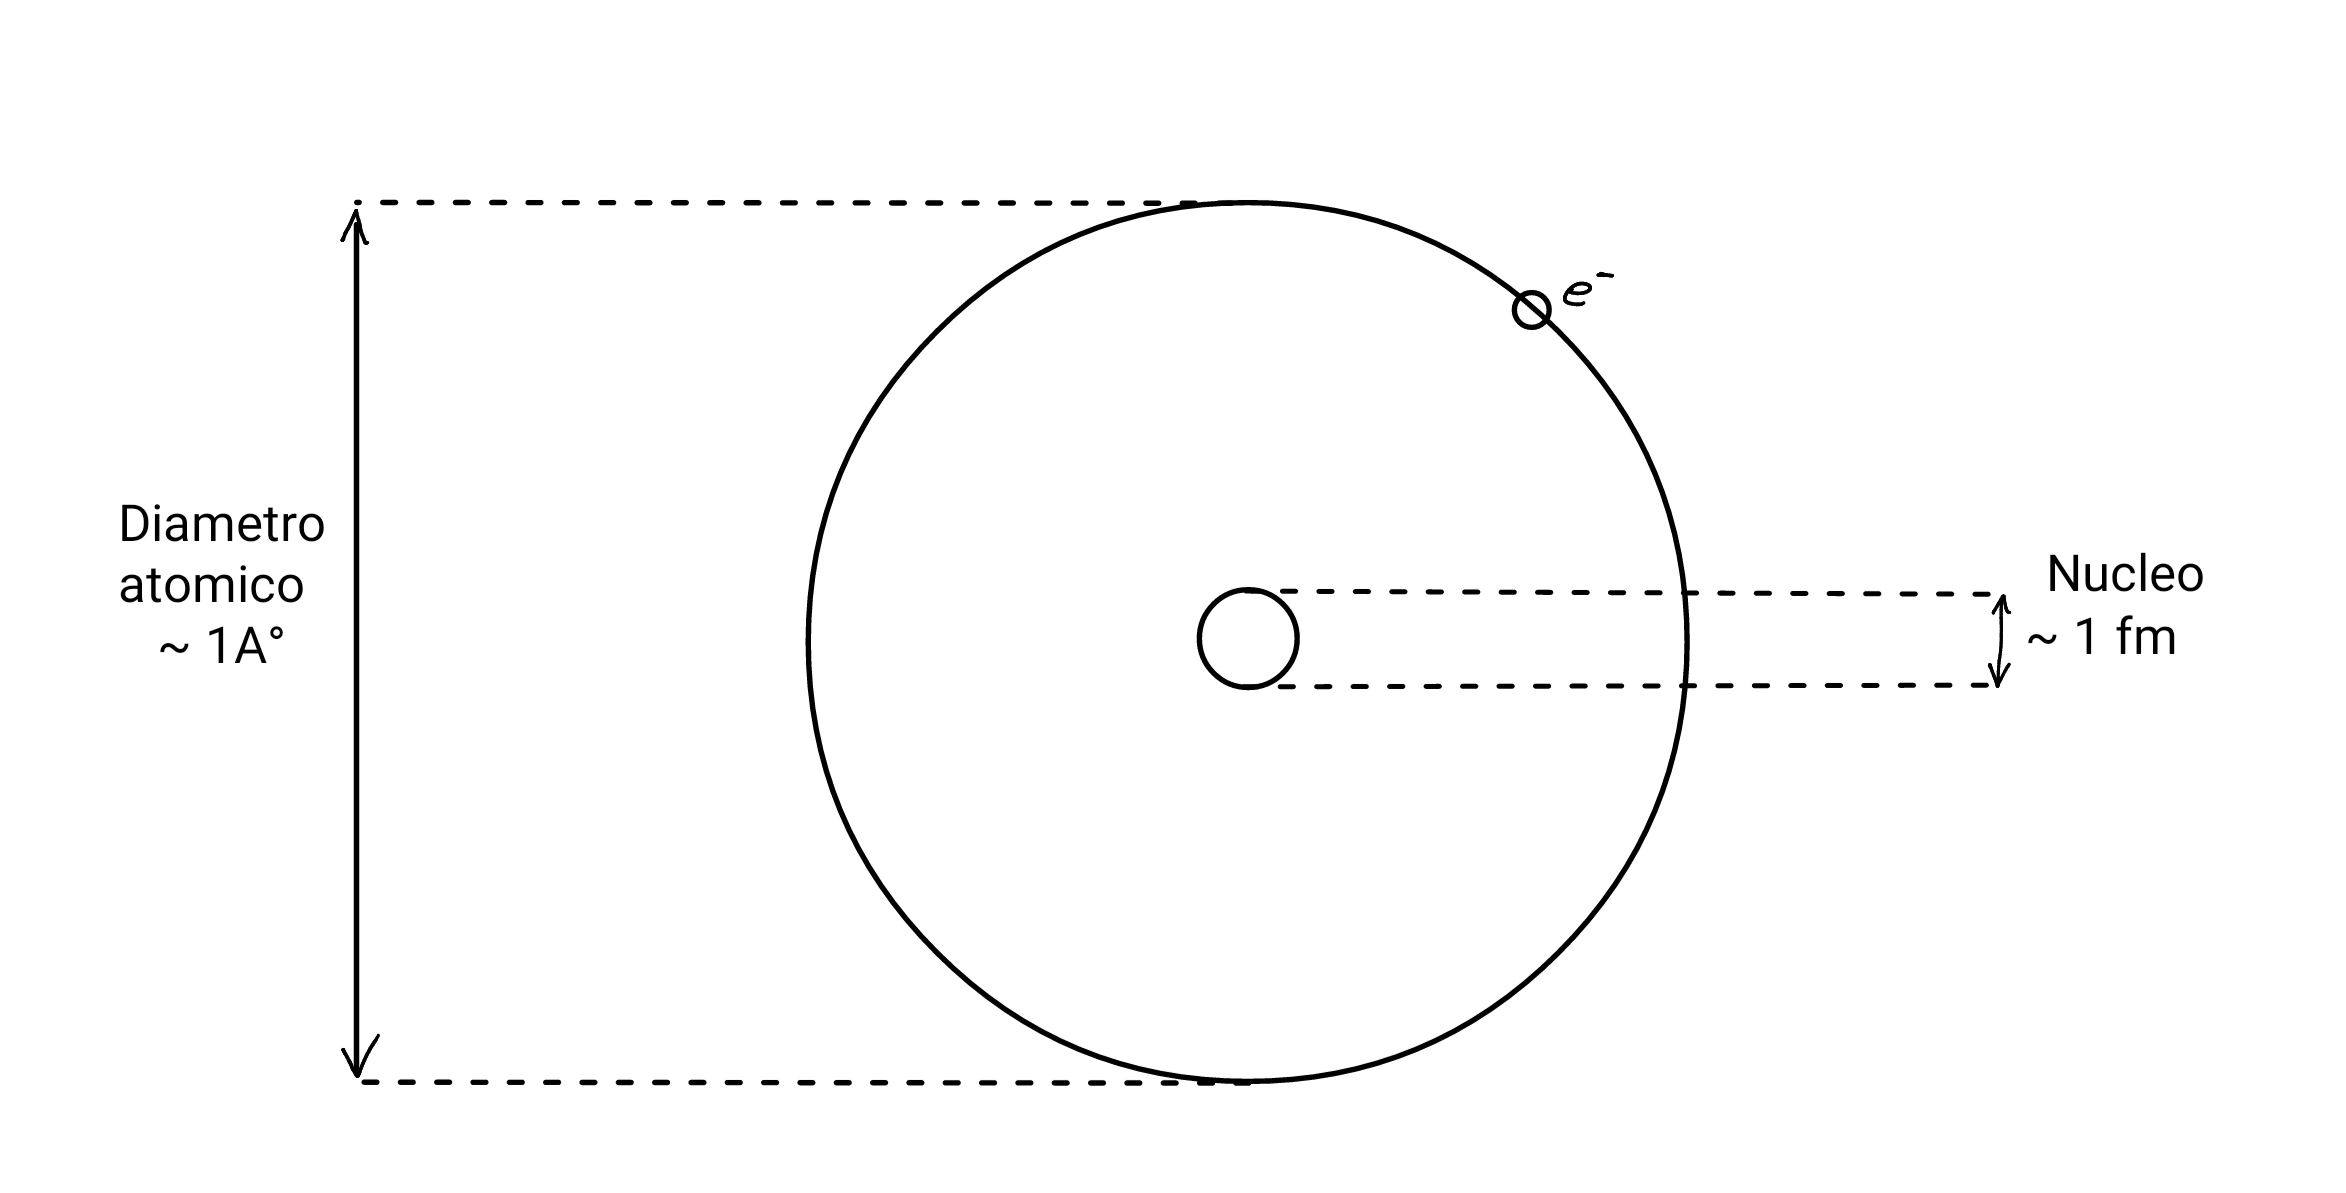
\includegraphics[width=0.6\textwidth]{immagini/dim-atomo.png}
	\caption{Dimensioni atomiche tipiche}
	\label{fig:atomo}
\end{figure}
Veniamo quindi agli scattering discussi, la situazione è modellizzata in Figura \ref{fig:rutherford}:
\begin{figure}[H]
	\centering
	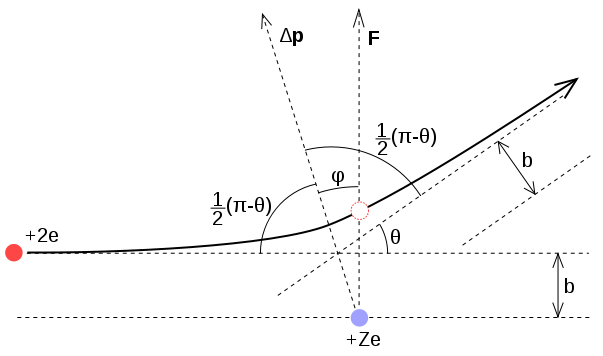
\includegraphics[width=0.8\textwidth]{immagini/rutherford.png}
	\caption{Schema dello scattering Rutherford.}
	\label{fig:rutherford}
\end{figure}
Per tutte le seguenti affermazioni viene considerto il centro scatterante come fisso (con massa molto maggiore del proiettile).
\paragraph{Interazione Columbiana.}
Inizialmente la particella ha una velocità $v_0$ che per la conservazione dell'energia e per simmetria deve essere uguale a quella finale $v_f$:
 \[
\left| \boldsymbol{v}_0 \right|  = \left| \boldsymbol{v}_f \right| 
.\] 
Si può trovare la variazione di impulso dopo interazione:
\[
	\Delta p = \left| \Delta \boldsymbol{p} \right| = \sqrt{\left( m \boldsymbol{v}_f - m \boldsymbol{v}_0 \right)^2} = m \sqrt{v_0^2 + v_0^2 -2v_0^2 \cos\left( \theta \right)} = 2m v_0 \sin\left( \frac{\theta}{2} \right)   
.\]
 
È utile anche ricordare la relazione che lega $\mu$ (angolo di riferimento che giace sul piano perpendicolare alla $\boldsymbol{v}_0$) all'elemento infinitesimo di sezione d'urto:
\[
d \sigma = b db d\mu
.\] 
Essendoci qua una simmetria sotto rotazioni attorno all'asse $\hat{v}_0$ possiamo integrare sull'angolo $\mu$ della relazione:
\[
d\sigma = 2 \pi b db
.\] 
Altra relazione differenziale che ci è utile adesso è: 
\[
\frac{\mbox{d} \sigma}{\mbox{d} \mu} = b db
.\] 
La sezione d'urto differenziale si può scrivere allora in funzione di $b\left( \theta \right)$ :
\[
	\frac{\mbox{d} \sigma}{\mbox{d} \Omega} = \frac{\mbox{d} \sigma}{\mbox{d}\mu \mbox{d}\cos\left( \theta \right) } = \frac{ b \mbox{d}b}{\mbox{d}\cos\left( \theta \right)} = - \frac{b \text{d}b}{ \sin\left( \theta \right) d \theta }  
.\]
Consideriamo adesso la variabile $\varphi$ nella Figura \ref{fig:rutherford} indice della posizione angolare dell'oggetto durante l'interazione, è definita appunto tra:
\[
\varphi_{\text{min}} = -\frac{\pi - \theta}{2} \le \varphi \le \frac{\pi -\theta}{2} = \varphi_{\text{max}}
.\] 
Possiaom giocarci la conservazione del momento angolare durante il processo sfruttando la variabile sopra definita come cordinata polare.
\[
	L_z = m \left( \boldsymbol{r \wedge \boldsymbol{v}}\right)_z = m \left[ \boldsymbol{r} \left( \dot{r} \hat{r} + r \dot{\varphi} \hat{\varphi}\right)\right]=
	mr^2\dot{\varphi}
.\] 
Quindi considerando anche il momento angolare iniziale abbiamo una prima relazione per parametrizzare il differenziale nel tempo:
\[
m v_0 b = m r^2 \frac{\mbox{d} \varphi}{\mbox{d} t} \quad \quad \implies \quad \quad dt = \frac{r^2}{b v_0} d\varphi
.\] 
Perche parametrizzare il tempo? Perche ci è utile per relazionare la variabile $b$ a $\theta$! Infatti la variazione di impulso calcolata sopra può essere scritta come:
\[
\left| \Delta \boldsymbol{p} \right| = \int_{-\infty}^{\infty} \left| \boldsymbol{F}_{\perp}\right| dt = 
\int_{-\infty}^{\infty} \left| \boldsymbol{F}\right| \cos\left( \varphi \right)  dt 
.\]
La forza citata è quella columbiana tra i due corpi:
\[
\left|\boldsymbol{F}\right| = \frac{zZe^2}{4 \pi \epsilon_0 r^2} 
.\] 
Mettiamo tutto nell'integrale (compreso il dt):
\[
	\left| \Delta \boldsymbol{p} \right| = \int_{\varphi_{\text{min}}}^{\varphi_{\text{max}}} \frac{zZe^2}{4 \pi \epsilon_0 b r^2} \frac{\cos\left( \varphi \right) }{b} \frac{r^2}{v_0} d \varphi 
	=  \frac{zZe^2}{2 \pi \epsilon_0 b v_0} \cos\left( \frac{\theta}{2} \right) 
.\] 
Senza mollare eliminiamo il $\left| \Delta \boldsymbol{p} \right|$ ricavato all'inizio:
\[
	2mv_0 \sin\left( \frac{\theta}{2} \right) = \frac{zZe^2}{2 \pi \epsilon_0 b v_0} \cos\left( \frac{\theta}{2} \right) 
.\] 
E le nostre fatiche vengono ripagate perche abbiamo la prima risposta:
\[
	b\left( \theta \right) = \frac{zZe^2}{4 \pi \epsilon_0 m  v_0^2} \cot\left( \frac{\theta}{2} \right) 
.\] 
È quindi possibile definire anche una minima distanza di urto centrale $d$ quando la cotangente è unitaria:
\[
	d = \frac{zZe^2}{4 \pi \epsilon_0 m  v_0^2} = \frac{zZ\left( \alpha \hbar c \right)}{T} \approx zZ \frac{1.44[\text{MeV}]}{T[\text{MeV}]} [\text{fm}]
	\quad \quad \implies \quad \quad b\left( \theta \right) = d \cot\left( \frac{\theta}{2} \right) 
.\] \label{eq:d-rutherford}
Apprezziamo la grandezza del risultato, siamo in grado di prevedere, note la carica e la massa del proiettile, la distanza ortogonale ($b$) tra i centri incidenti dal momento che scegliamo l'angolo di osservazione $\theta_0$ (o meglio, tutto ciò che arriva all'osservatore è partito da una posizione con parametro di impatto noto).\\
Si può infine trovare la sezione d'urto Rutherford differenziale come:
\[
	\frac{\mbox{d} \theta}{\mbox{d} \Omega} = -\frac{b db}{\sin\left( \theta \right) d \theta} =
	-\frac{b}{2 \cos\left( \frac{\theta}{2} \right) \sin\left( \frac{\theta}{2} \right)} \cdot \frac{d}{2}\left( \frac{d \left( \cot\left( \frac{\theta}{2} \right)\right)}{d \theta} \right) = 
	\ldots = \frac{d^2}{16 \sin^{4}\left( \frac{\theta}{2} \right) } 
.\] 

\paragraph{Interazione con sfera rigida}
In questo caso basta sfruttare alcune semplici considerazioni geometriche:
\[
	\frac{\text{d}\sigma}{\text{d} b} = 2 \pi b \quad \quad \text{ con } \quad b<R 
.\] 
A fare la differenza qua è la semplice definizione di $\theta$:
\[
	\frac{b}{R} = \sin\left( \frac{\pi - \theta}{2} \right) = \cos\left( \frac{\theta}{2} \right)  \implies b = R \cos\left( \frac{\theta}{2} \right) 
.\] 

% 2.b.21
\subsection[]{Calcolare la minima distanza fra le due particelle in uno scattering Rutherford.}
Definiamo $v_m$ come la velocità del proiettile nell'istante in cui ha raggiunto la distanza minima $x$. Sfruttando la conservazione dell'energia e del momento angolare si ottiene:
\[	
	\frac{1}{2}m v_0^2 = \frac{1}{2} m v_f^2 + \frac{zZe^2}{4 \pi \epsilon_0 x}\\
.\] 
\[
	mv_0b = m v_m x
.\]
Si ricava $v_m$ dalla seconda sostituendola nella prima, ne risulta una equazione del secondo grado per $x$:
 \[
	 x^2 - d \cdot x - b^2 = 0 \implies x = \frac{d}{2} \left( 1 + \frac{1}{\sin\left( \frac{\theta}{2} \right) } \right) 
.\] 
%2.b.22
\subsection[]{Calcolare l'energia minima affinché un protone possa avere una interazione forte "toccando" un nucleo di ${}^{12}C$ o di ${}^{28} Si$.}
È inanzitutto necessario per risolvere il problema di minimo considerare l'urto centrale: $b = 0$.\\ 
In tal caso l'angolo di scatternig è $\theta = \pi$ e $x = d$ dove $d$ è la distanza tra i nuclei aventi raggio:
\[
	R = \left( 1.25 A^{1 /3} + 2 \right) \text{fm} 
.\] 
L'energia minima è allora proprio l'energia potenziale necessaria ad arrivare alla distanza $d$:
 \[
	 E_{\text{min}} = \frac{zZe^2}{4 \pi \epsilon_0 \left( R_1 + R_2 \right) } 
.\] 
O molto più semplicemente (vista la fatica fatta in precedenza per \hyperref[eq:d-rutherford]{definire d}:
\[
	d = \left( R_1 + R_2 \right) \approx zZ\frac{1.44 [\text{MeV}]}{T[\text{Mev}] } [\text{fm}] \implies T = zZ\frac{1.44}{\left( R_1+R_2\right) } [\text{MeV}]
.\] 
Mettendo i numeri si ha:
\[
E_{\text{C}} \approx 1.4 \text{MeV} ,\quad \quad 
E_{\text{Si}} = 11.2 \text{MeV}
.\] 

%2.b.23
\subsection[]{Discutere le differenze tra lo scattering di Rutherford (particelle $\alpha$ su nuclei) e lo scattering di elettroni su bersaglio puntiforme.}
La differenza principale è che gli elettroni si muovono solitamente a velocità relativistiche, questo invalida i conti fatti prima. Nel caso discusso quindi è necessario tirare in ballo la sezione d'urto Mott.

%2.b.24
\subsection[]{Cercando i dati nelle apposite tabelle (reperibili sul web ) si indichino gli stati finali e si calcoli il Q-valore per i decadimenti delle seguenti specie instabili: ${}^8B, {}^{39}Ar, {}^{7}Be, {}^{64}Cu, {}^{76}Ge$. }
Per rispondere a questa domanda è necessario ricordarsi la natura dei \hyperref[sec:decadimenti]{Decadimenti} ed avere sottomano il Nuclear Wallet Card.
\paragraph{Isotopo del Boro}
\label{par:8B}
\[
	\ce{\ce{^{8}_{5}B_{3}} ->[\epsilon] \ce{^{8}_{4}\text{Be}_{4}} ->[\alpha] \ce{^{4}_{2}\text{He}^{2-}_{2}} } 
.\]
\[
	\Delta Q_{\epsilon} = \Delta_{A, Z} - \Delta_{A, Z-1} \approx 18 \text{ Mev} \quad \quad  
\]
\[
	\Delta Q_{\alpha} = ( 4m_u +  \Delta_{A,Z-1}) - \left( \Delta_{A-4, Z-2} + 4m_u + \Delta _{\alpha} \right) \approx 0.1 \text{ MeV}
.\] 
Quindi l'energia complessiva del processo è 
\[
	\Delta Q_{\epsilon}+ \Delta Q_{\alpha} \approx 18.1 \text{ MeV}.
\]
Notare che in questo caso particcolare i prodotti di decadimento $\alpha$ e $\ce{^{4}_{2}\text{He}^{2-}_{2}}$ hanno approssimativamente la stessa massa.
\paragraph{Isotopo dell'Argon}
\label{par:39Ar}
\[
	\ce{\ce{^{39}_{18}\text{Ar}_{21}}  ->[\beta^-] \ce{^{39}_{19}K_{20}}}
.\] 
\[
	\Delta Q_{\beta^-} = \Delta_{A,Z} - \Delta_{A, Z+1} = 0.57 \text{ MeV} 
.\] 
\paragraph{Isotopo del Berillio}%
\label{par:7Be}
\[
	\ce{\ce{^{7}_{4}\text{Be}_{3}} ->[\epsilon] \ce{^{7}_{3}\text{Li}_{4}} }
.\] 
\[
\Delta Q_{\epsilon} = \Delta_{A, Z} - \Delta_{A, Z-1} \approx 1.861 \text{ MeV}
.\] 
\paragraph{Isotopo del Rame}%
\label{par:64Cu}
Nelle tabelle sono indicate due possibilità, esaminiamo entrambe:
\[
	\ce{ \ce{^{64}_{30}\text{Zn}_{34}} <-[\beta^-][38.5 \%] \text{ } \ce{^{64}_{29}\text{Cu}_{35}} \text{ } ->[\epsilon][61.5\%] \ce{^{64}_{28}\text{Ni}_{36}} }
.\] 
Senza essere ripetitivi (stesse cose viste sopra) si riportano i risultati:
\[
\Delta Q_{\epsilon} = 1.67 \text{ MeV}
.\] 
\[
\Delta Q_{\beta^-} = 0.68 \text{ MeV}
.\] 

\paragraph{Isotopo del Germanio}%
\label{par:76Ge}
\[
	\ce{^{76}_{32}\text{Ge}_{44}} \implies \tau_{1 /2} \sim 2 \cdot 10^{21} 
.\]
Al gran sasso si studia il decadimento $\beta^- \beta^-$ di Questo isotopo (nome in codice GERDA).
\paragraph{Nota:} I conti della domanda sono stati fatti senza calcolatore per allenamento, siete fortemente invitati a fare lo stesso e riportare gli errori a chi ha accesso al source code.

% 2.b.25
\subsection[]{Cercando i dati nelle apposite tabelle (reperibili sul web) si trovino i Q-valori per le reazioni 
\begin{enumerate}
	\item $n + {}^{154}Gd \implies \gamma + {}^{155}Gd$ 
	\item $n + {}^{155}Gd \implies \gamma + {}^{156}Gd$
\end{enumerate}
}
\[
	\Delta Q_1 = \left( m_n + 154 m_u + \Delta_{154, 64} \right) - \left( 155m_u + \Delta_{154, 64 } \right) \approx 6.43 \text{ MeV} 
.\]
\[
	\Delta Q_2 = \ldots \approx m_{n} - m_{u} + \Delta_{155,64}-\Delta_{156,64} \approx 7.4 \text{ MeV} 
.\] 

% 2.b.26
\subsection[]{Dimostrare che $\frac{d^3 p  }{2E}$ è un invariante relativistico effettuando esplicitamente la trasformazione di Lorentz (si consideri il boost lungo un asse, per esempio l'asse x)}
Facciamo questo boot lungo x:
\begin{align*}
	\frac{\mbox{d}^3 \boldsymbol{P}'}{2E'}  =& \frac{dP'_x dP'_y dP'_z}{2Ex'} = \\
	=& \frac{\gamma d\left( P_x + \beta E \right)dP_y dP_z }{2 \gamma\left( E + \beta P_x \right)} = \\
	=& \frac{ \left[ dP_x + \beta d \sqrt{P_x^2 + m^2}\right]dP_y dP_z  }{2\left( E + \beta P_x \right) } = \\ 
	=& \frac{\left( dP_x + \beta\frac{2P_x dP_x}{2\sqrt{P_x^2 + m^2} } \right)dP_y dP_z }{2\left( E + \beta P_x \right)} = \\
	= & \frac{\mbox{d}^3 \boldsymbol{P}}{2E}
.\end{align*}

% 2.b.27
\subsection[]{Dimostrare che 
\[
d^{4}P \delta\left( P^2-m^2 \right) \theta\left( P_0 \right) = \frac{d^3 \boldsymbol{P} }{2E}
\]
e sfruttare questo risultato per semplificare la scrittura dell’elemento infinitesimo dello spazio dei 4-impulsi di N particelle emergenti dopo la collisione di due particelle (oppure dopo il decadimento di una particella).}
È sufficiente rimembrare una delle proprietà della $\delta$:
\[
	\delta\left( f\left( x \right)  \right) = \sum_{j} \frac{\delta\left( x-x_j \right) }{\left| \left[ f'\left( x \right)  \right]_{x = x_j} \right| }
.\] 
Da inserire opportunamente nella espressione a sinistra dell'uguale nella richiesta: dobbiamo ricordare che $P$ è in realtà un quadrivettore.
\begin{align*}
	d^{4}P \cdot \delta\left( P^2-m^2 \right) \theta\left( P_0 \right) =& d^4P\cdot  \delta\left(\boldsymbol{P}^2 - P_0^2 - m^2 \right) \theta\left( P_0 \right)  = \\
	=& d^4 P \cdot  \theta\left( P_0 \right) \left[ \frac{\delta\left( P_0 - E \right) }{\left| \left[ 2P_0 \right]_{P_0 = E} \right| } + 
		\frac{\delta\left( P_0 + E \right) }{\left| \left[ 2P_0 \right]_{P_0 = -E}  \right| } \right] =\\
		=& d^4P \frac{\delta\left( P_0 - E \right)}{2E} = \frac{d^3 \boldsymbol{P}}{2E}   
.\end{align*}
\paragraph{Nota:}%
Stiamo parlando di distribuzioni, la notazione leggera utilizzata nasconde significati matematici profondi e non scontati (vedi corso di metodi matematici per la fisica II).

% 2.b.28
\subsection[]{Dimostrare che nel centro di massa l’elemento infinitesimo dello spazio dei 4-impulsi, nel caso di 2 sole particelle nello stato finale, si scrive come $\frac{|\boldsymbol{p_{cm}}}{4\sqrt{s}} d\Omega_{cm}.$}
Ricordiamo la forma dell'elemento infinitesimo dello spazio delle fasi:
\[
	dL_p = \left[ d^4P_1 \cdot \delta\left( P_{0,1}^2 - \boldsymbol{P}_1^2 - m_1^2 \right) \cdot \theta\left( P_{0,1} \right) \right] \cdot \ldots 
	\left[ \cdot d^4P_n \cdot \delta\left( P_{0,n}^2 - \boldsymbol{P}_n^2 - m_n^2 \right) \cdot \theta\left( P_{0,n} \right) \right] \cdot 
	\delta^4\left(  P_{in}-\sum_{i}P_i  \right) 
.\]
Che utilizzando la risposta alla domanda precedente si riscrive come:
\[
dL_p = \frac{\mbox{d}^3 \boldsymbol{P}_1}{2E_1} \ldots \frac{\mbox{d}^3 \boldsymbol{P}_n}{2E_n} \delta^4\left( P_{in}-\sum_{i}P_i \right) 
.\] 
Decisamente più carino.\\
Se si hanno due prodotti definiamo le loro masse come $m_1$ e  $m_2$, l'energia del centro di massa $\sqrt{s}$ e ricordiamo che il 3-impulso totale nel centro di massa è nullo. L'elemento infinitesimo $dL_p$ si scrive come:
\begin{align*}
	dL_p =& \frac{d^3 \boldsymbol{P}_1}{2E_1} \frac{d^3 \boldsymbol{P}_2}{2E_2} \cdot \delta^4\left(P_{\text{in}} - P_1 - P_2 \right) = \\ 
	= & \frac{d^3 \boldsymbol{P}_1}{2E_1} \frac{d^3 \boldsymbol{P}_2}{2E_2} \cdot \delta\left( \sqrt{s}-E_1-E_2\right) \cdot 
	\delta^3\left( \boldsymbol{0} + \boldsymbol{P}_1 + \boldsymbol{P}_2 \right) = \\
	= & \frac{ d \boldsymbol{P}_1 }{4E_1E_2} \cdot \delta\left( \sqrt{s}-E_1-E_2\right)   
\end{align*}
Passando in cordinate spefiche:
\[
	dL_p = \frac{P_1^2 dP_1 d \Omega_1 }{4E_1E_2} \cdot \delta\left( \sqrt{s} -E_1-E_2  \right) 
.\]
Possiamo adesso sfruttare il fatto che nel centro di massa l'impulso totale è nullo, chiamiamo $P_{\text{cm}}$ l'impulso della particella singola (le due particelle hanno in modulo lo stesso impulso in questo sistema $\left| \boldsymbol{P}_1 \right| = \left| \boldsymbol{P}_2 \right| = P_{\text{cm}}$):
\[
	\sqrt{s}= \sqrt{P_{\text{cm}}^2 + m_1^2} + \sqrt{ P_{\text{cm}}^2 + m_2^2} 
.\] 
Che può essere risolta ( Hint: servono due elevazioni al quadrato) per $P_{\text{cm}}$ :
\[
	P_{\text{cm}} = \sqrt{\frac{\left( s - \left( m_1+m_2 \right)^2 \right) \left( s - \left( m_1 - m_2 \right)^2 \right)}{4s}} 
.\]
Non esplicitiamo $P_{\text{cm}}$ nei calcoli a seguire, è bene però sappere che può essere scritto in funzione di variabili più "comuni". La relazione sopra sarà sfruttata al secondo passaggio del seguente calcolo.
\begin{align*}
	dL_p =& \frac{P_1^2 dP_1 d \Omega_1}{4E_1E_2} \cdot \delta\left( \sqrt{s} - \sqrt{P_1^2 + m_1^2} - \sqrt{P_2^2 + m_2^2}  \right) \\
	=& \frac{P_1^2 dP_1 d \Omega_1}{4E_1E_2} \cdot 
	\frac{\delta\left(P_1-P_{\text{cm}}\right)}{\left|\left[\frac{\mbox{d}}{\mbox{d}P_1}\left(\sqrt{s}-\sqrt{P_1^2+m_1^2}-\sqrt{P_1^2+m_2^2}\right)\right]_{P_1=P_{\text{cm}}}\right|} = \\
	=& \frac{P_1^2 dP_1 d \Omega_1}{4E_1E_2} \cdot \frac{ \delta \left( P_1-P_{\text{cm}} \right) }{ \left| \left[ \frac{P_1}{E_1}+\frac{P_1}{E_2} \right]_{P_1=P_{\text{cm}}} \right|}=\\
	=& \frac{P_1^2 dP_1 d \Omega_1}{4E_1E_2} \cdot \frac{\delta\left(P_1-P_{\text{cm}}\right)}{P_{\text{cm}} \frac{E_1 + E_2}{E_1E_2}} = \\
	=& \frac{P_{\text{cm}} }{4\sqrt{s}} d\Omega_{1}
\end{align*}
Noto l'impulso delle particelle nel centro di massa (o, se si vuole, $\sqrt{s}, m_1, m_2$) si ha che l'elemento infinitesimo dello spazio delle fasi dei due prodotti dipende solo dall'angolo solido di un prodotto (che in caso di isotropia spaziale come qua è l'opposto di $\Omega_2$). Questo è molto utile per la sezione d'urto differenziale ad esempio.
\[
	\frac{\mbox{d} \sigma}{\mbox{d} \Omega_1} = f_{\text{urto}}\left( \Omega_1 \right) \frac{P_{\text{cm}}}{4\sqrt{s} }
.\] 

% 2.b.29
\subsection[]{Nel caso di 3 particelle nello stato finale di una reazione, dimostrare che fra il quadrato della massa invariante di due di esse e l'energia della terza (nel centro di massa) sussite una relazione lineare.}
Prendiamo la massa invariante citata $\sqrt{s_{12}}$ e l'energia della restante paticella come $E_3$, con ovvio significato dei simboli si ha (definizione di massa invariante):
\[
	s_{12} = \left( P_1 + P_2 \right)^2
.\] 
Che per la conservazione dell'energia e dell'impulso si può scrivere come:
\[
	s_{12} = \left( P_{\text{in}} - P_3 \right)^2 = P_{\text{in}}^2 + P_3^2 - 2 P_{\text{in}}P_3 =s + m_3^2 - 2 \sqrt{s}E_3 
.\] 
Ecco la relazione lineare.

% 2.b.30
\subsection[]{Come si trasforma una funzione di distribuzione del 3-impulso 
\[
	f\left( \boldsymbol{p} \right)d^3 \boldsymbol{p}
\]
di una particella per una trasformazione di Lorentz?}
Premessa: misurare in un sistema la funzione di distribuzione del 3-impulso significa misurare il numero di eventi dn nell'elemento di volume nello spazio degli impulsi $dn = f\left( \boldsymbol{P} \right) d^3 \boldsymbol{P}$. È inoltre naturale che il numero di eventi registrati deve essere lo stesso in ogni sistema di riferimento 
\[
dn = f\left( \boldsymbol{P} \right) d^3 \boldsymbol{P} =  f\left( \boldsymbol{P}' \right) d^3 \boldsymbol{P}' = dn'
\]
Abbiamo dimostrato anche che 
\[
\frac{d^3 \boldsymbol{P}}{2E} 
.\] 
è un invariante relativistico, quindi si può concludere:
\[
	\frac{E}{E} f\left( \boldsymbol{P} \right) d^3 \boldsymbol{P} = \frac{E'}{E'} f\left( \boldsymbol{P}' \right) d^3 \boldsymbol{P}' \quad \implies \quad 
	f\left( \boldsymbol{P}' \right) = \frac{E}{E'} f\left( \boldsymbol{P} \right) 
.\] 

% 2.b.31
\subsection[]{Come si trasforma una funzione di distribuzione nello spazio delle fasi 
\[
	f\left(\boldsymbol{p},\boldsymbol{r}\right)d^3 \boldsymbol{p} \ d^3 \boldsymbol{r} 
\]
di una particella per una trasformazione di Lorentz?}
È necessario notare che anche qua il numero di eventi $dn$ nel volume infinitesimo dello spazio delle fasi si deve conservare come sopra, ragionando quindi allo stesso modo si trova la legge di trasformazione richiesta.\\
Mettiamoci per utilità nel sistema in cui la particella è a riposo e consideriamo un boost lungo uno dei 3 assi di riferimento, possiamo sfruttare la contrazione delle lunghezze
\[
\text{d}^3 \boldsymbol{r}' =\frac{\text{d}^3\boldsymbol{r}}{\gamma} =  \frac{\text{d}^3\boldsymbol{r}}{E'} mc^2 = \frac{\text{d}^3\boldsymbol{r}}{E'} E
.\] 
Quindi $Ed^3 \boldsymbol{r}$ è un invariante relativistico. Avendo trovato che anche $d^3 \boldsymbol{P} / E$ è invariante si ha che
\begin{align*}
	dn = f\left( \boldsymbol{P}, \boldsymbol{r} \right) \text{d}^3 \boldsymbol{P} \text{d}^3 \boldsymbol{r} =  f\left( \boldsymbol{P}', \boldsymbol{r}' \right) 
	\text{d}^3 \boldsymbol{P}' \text{d}^3 \boldsymbol{r}' = dn' & \quad \quad
	\text{Invarianza del numero di eventi} \\
	\frac{\text{d}^3 \boldsymbol{P}}{E} E \text{d}^3 \boldsymbol{r} =
	\frac{\text{d}^3 \boldsymbol{P}'}{E'} E' \text{d}^3 \boldsymbol{r}' & \quad \quad 
	\text{Invarianti trovati sopra}
.\end{align*}
Dalle quali deriva l'invarianza di $f\left( \boldsymbol{P}, \boldsymbol{r} \right)$.

% 2.b.32
\subsection[]{Dimostrare che se la probabilità di decadimento di una particella per unità di tempo non dipende dal tempo, la probabilità di trovare la particella non decaduta al tempo t segue una legge esponenziale.}
Sia $S\left( t \right) $ la probabilità di trovare la particella al tempo $t$, considerando la invece la probabilità $P\left( t \right)$ di decadere dopo l'unità di tempo $dt$ si ha (per ipotesi):
 \[
	 \frac{P\left( dt \right)}{dt}= \frac{1}{\tau} \text{ (costante)} \implies  S\left( dt \right) = 1 - \frac{dt}{\tau}
.\] 
Quindi all'istante $t + dt$ si ha (per le regole delle probabilità combinate):
\[
	S\left( t + dt \right) = S\left( t \right) S\left( dt \right) = S\left( t \right) \left( 1 - \frac{dt}{\tau} \right) 
.\] 
Che ha come soluzione proprio un esponenziale (vedi \hyperref[sec:2.b.5]{Domanda 2.b.5}):
\[
	S\left( t \right) = e^{- t / \tau}
.\] 

% 2.b.33
\subsection[]{ Dire quali fra le seguenti particelle sono soggette ad interazioni forti: $ p, \overline{p} $, $\pi^{+}, \pi^{-}, \mu^{+}, \mu^{-}, e^{+}$, $e^{-}$, $\alpha,$ Nucleo di Azoto, $\nu, \overline{\nu}$ }
\label{sec:2.b.33}
Solo gli adroni (composti da Quark) possono fare interazione forte, quindi la risposta è: $p$ , $\overline{p}$ , $\pi^{+}$ , $\pi^{-}$ , $\alpha$ , Nucleo di Azoto.

\subsection[]{Pioni neutri, di energia E nel sistema del laboratorio, decadono in due fotoni. La distribuzione è isotropa ne centro di massa. Si calcoli la distribuzione dell’energia di uno dei due fotoni nel laboratorio e gli angoli, rispetto alla direzione di volo del pione, dei due fotoni nel sistema del laboratorio in funzione dell’angolo nel sistema del centro di massa.}
\begin{figure}[H]
	\centering
	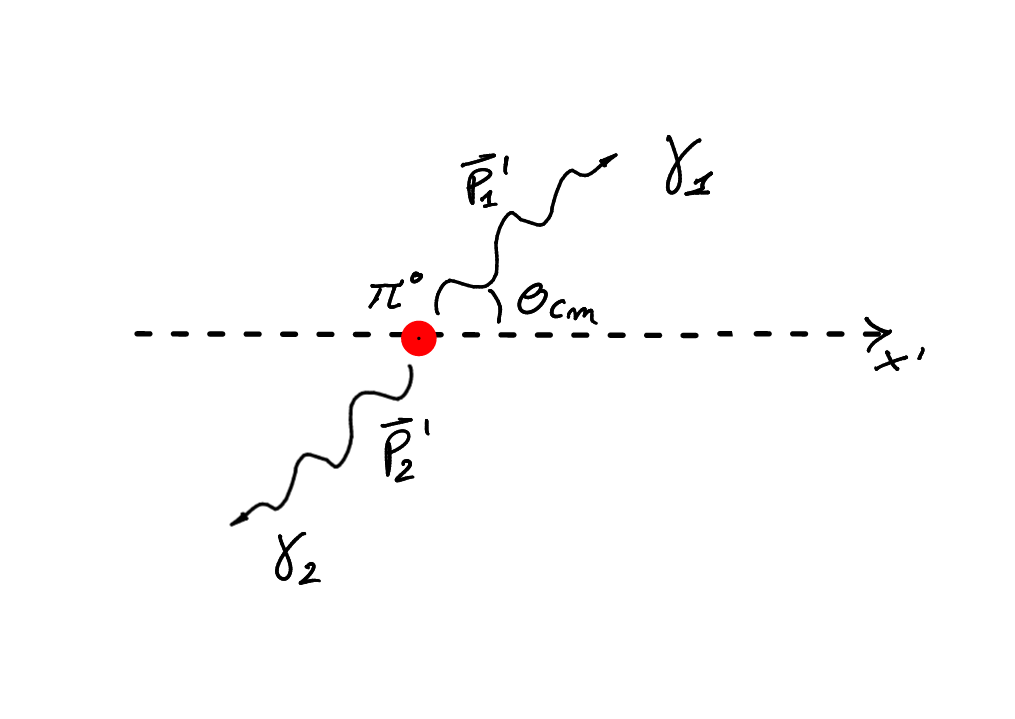
\includegraphics[width=0.35\textwidth]{immagini/decadimento-pi1.png}
	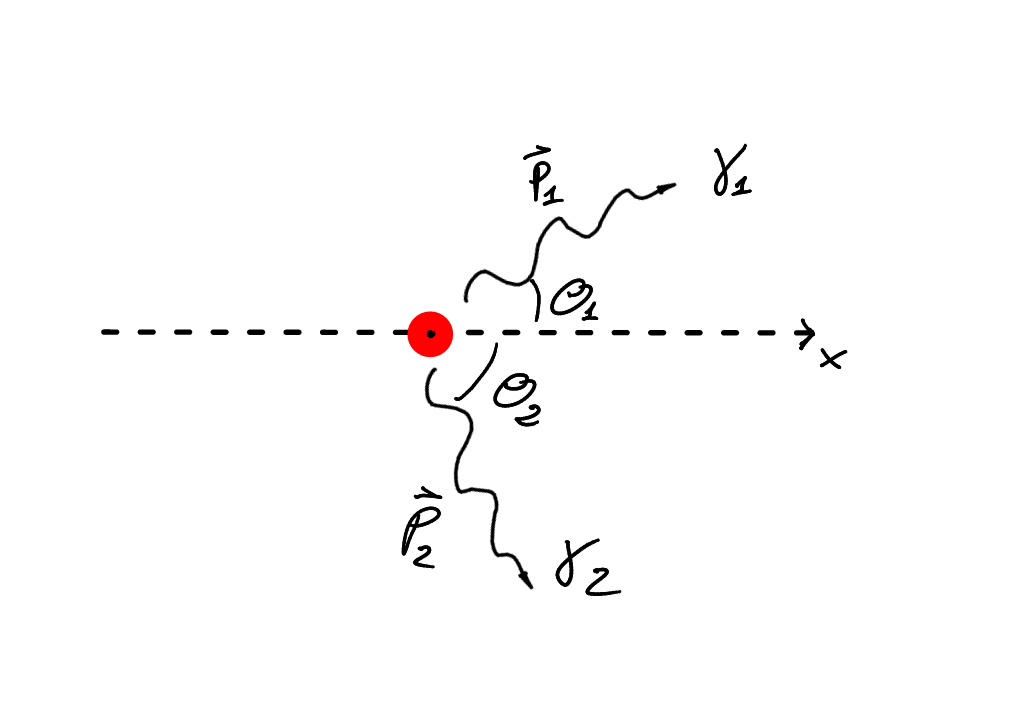
\includegraphics[width=0.35\textwidth]{immagini/decadimento-pi2.png}
	\caption{Decadimento del $\pi^0$ in due fotoni: a sinistra nel centro di massa e a destra nel sistema del laboratorio.}
	\label{fig:Decadimento del Pione in fotoni.}
\end{figure}
Fissando idee e notazione come in Figura \ref{fig:Decadimento del Pione in fotoni.} procediamo al calcolo richiesto.
\[
	\ce{\ce{\pi} -> \ce{\gamma} + \ce{\gamma}}
.\] 
La massa del $\pi^0$ è 134.96 MeV, assumiamo che nel laboratorio questo si muova con velocità $\beta$ nell'istante precedente al decadimento. Nel sistema del $\pi^0$ si ha:
 \[
P_1' = \frac{m}{2} \cdot 
\begin{pmatrix}
	1 \\
	\cos\left( \theta_{\text{cm}} \right) \\
	\sin\left( \theta_{\text{cm}} \right) \\
	0
\end{pmatrix} \quad \quad \quad 
P_2' = \frac{m}{2}\cdot 
\begin{pmatrix} 
	1 \\
	-\cos\left( \theta_{\text{cm}}\right) \\
	- \sin\left( \theta_{\text{cm}} \right) \\
	0
\end{pmatrix} 
.\] 
Essendo inoltre la distrubuzione di prodotti isotropa nel centro di massa possiamo scrivere:
\[
	\frac{\text{d} \Gamma}{\text{d}\Omega_{\text{cm}}} = \frac{\Gamma}{4 \pi} \quad \quad \implies \quad \quad 
	\frac{\text{d} \Gamma}{\text{d}\cos\left( \theta_{\text{cm}} \right) } = \frac{\Gamma}{2}
.\] \label{eq:isotropia}
Nel laboratorio si ha invece:
\[
P_1 = E_1 \cdot 
\begin{pmatrix}
	1 \\
	\cos\left( \theta_1 \right) \\
	\sin\left( \theta_1 \right) \\
	0
\end{pmatrix} \quad \quad \quad 
P_2 = E_2\cdot
\begin{pmatrix} 
	1 \\
	\cos\left( \theta_2 \right) \\
	 \sin\left( \theta_2 \right) \\
	0
\end{pmatrix} 
.\] 
È possibile limitare le energie dei prodotti nel laboratorio tramite una trasformazione di Lorentz:
\begin{align*}
	E_1=&\gamma\frac{m}{2}\left(1+\beta\cos\left(\theta_{\text{cm}}\right)\right)&
		\quad E_2=&\gamma\frac{m}{2}\left(1-\beta\cos\left(\theta_{\text{cm}}\right)\right)\\
	P_{1,x} = E_1 \cos\left( \theta_{1} \right) =& \gamma \frac{m}{2} \left( \beta + \cos \left(\theta_{\text{cm}} \right) \right)   &
		\quad P_{2,x} = E_2 \cos\left( \theta_2 \right) =& \gamma \frac{m}{2} \left( \beta - \cos\left( \theta_{\text{cm}} \right)  \right) \\ 
	P_{1,y} = E_1 \sin\left( \theta_1 \right) =& \frac{m}{2}\sin\left( \theta_{\text{cm}}\right) &
		\quad P_{2, y} =E_2\sin\left( \theta_2 \right) =& - \frac{m}{2} \sin\left( \theta_{\text{cm}}\right) 
.\end{align*}
Guardando alla prima colonna facendo variare il $\cos\left( \theta_{\text{cm}} \right) $ con la fantasia è facile vedere che:
\[
	\gamma \frac{m}{2}\left( 1 - \beta \right) \le E_1 \le \gamma \frac{m}{2} \left( 1 + \beta \right) 
.\] 
Possiamo adesso calcolarci come è distribuita l'energia $E_1$ (della particella 1 nel laboratorio):
\[
	\frac{\mbox{d} \Gamma}{\mbox{d} E_1} = 
	\frac{\mbox{d} \Gamma}{\mbox{d} \cos\left( \theta_{\text{cm}} \right) } \frac{\mbox{d} \cos\left( \theta_{\text{cm}} \right) }{\mbox{d} E_1} =
	\frac{\Gamma}{2} \frac{2}{m \gamma \beta} = \frac{\Gamma}{m \gamma \beta}
.\] 
La distribuzione è quindi piatta (non dipende da $E_1$) e ben normalizzata se integrata nei limiti di $E_1$.\\
Per quanto riguarda la seconda richiesta procediamo calcolando la distribuzione angolare di uno dei fotoni.
Per farlo possiamo sfruttare ancora le trasformazioni di Lorentz di cui sopra isolando gli angoli nel laboratorio (essenzialmente la risposta al quesito è questa):
\begin{align*}
	\cos\left(\theta_1\right)=&\frac{P_{1,x}}{E_1}=\frac{\beta+\cos\left(\theta_{\text{cm}}\right)}{1+\beta\cos\left(\theta_{\text{cm}}\right)}\quad&  
	\cos\left(\theta_2\right)=&\frac{P_{2,x}}{E_2}=\frac{\beta-\cos\left(\theta_{\text{cm}}\right)}{1-\beta\cos\left(\theta_{\text{cm}}\right)} \\  
	\sin\left(\theta_1\right)=&\frac{P_{1,y}}{E_1}=\frac{\sin\left(\theta_{\text{cm}}\right)}{\gamma\left(1+\beta\cos\left(\theta_{\text{cm}}\right)\right)}\quad&
	\sin\left(\theta_2\right)=&\frac{P_{1,y}}{E_2}=\frac{-\sin\left(\theta_{\text{cm}}\right)}{\gamma\left(1-\beta\cos\left(\theta_{\text{cm}}\right)\right)}
.\end{align*}
Dalla prima in alto si ricava la cosa che ci serve: $\cos\left( \theta_{\text{cm}} \right)$ in funzione di $\cos\left( \theta_1 \right)$:
\[
	\cos\left( \theta_{\text{cm}} \right) = \frac{-\beta + \cos\left( \theta_1 \right) }{1 - \beta\cos\left( \theta_1 \right) }
.\] 
Sfruttiamo adesso l'isotropia nel centro di massa:
\begin{align*}
	\frac{\text{d}\Gamma}{\text{d}\cos\left( \theta_{1} \right) } =&
	\frac{\mbox{d}\Gamma}{\mbox{d}\cos\left(\theta_{\text{cm}}\right)}\frac{\mbox{d}\cos\left(\theta_{\text{cm}}\right)}{\mbox{d}\cos\left(\theta_1\right)}=\\
	=&\frac{\Gamma}{2}\frac{1-\beta\cos\left(\theta_1\right)-(-\beta)(-\beta+\cos(\theta_1))}{\left(1-\beta\cos(\theta_1)\right)^2} =\\
	=& \frac{\Gamma}{2}\frac{1-\beta^2}{\left( 1-\beta\cos\left(\theta_1\right)\right)^2}=\\
	=&\frac{\Gamma}{2\gamma^2}\frac{1}{\left(1-\beta\cos(\theta_1)\right)^2}
.\end{align*}
Nell'ultima equazione si evidenzia come siano prediletti angoli piccoli (funzione crescente al tendere di $\ce{\ce{\theta_1} -> 0 }$).\\
Infine possiamo dire qualcosa in più sulla differenza degli angoli nel laboratorio, nonchè "l'apertura" del cono formato dalla direzione dei due fotoni nel lab:
\[
	\sin\left( \theta_1-\theta_2 \right) = \sin\left( \theta_1 \right) \cos\left( \theta_2 \right) -\sin\left( \theta_2 \right) \cos\left( \theta_1 \right) =
	\frac{2 \beta\sin\left( \theta_{\text{cm}} \right) }{\gamma\left( 1-\beta^2\cos^2\left(\theta_{\text{cm}}\right)\right) }
.\]
Questa funzione vista la dipendenza da $\beta$ fa cose diverse a seconda della velocità del $\pi^0$. 

%2.b.35
\subsection[]{ Calcolare la funzione di distribuzione in energia ed in angolo nel sistema del laboratorio di un fascio di neutrini o di muoni prodotto nel decadimento di pioni carichi di energia 14 GeV.}
\[
	\ce{\ce{\pi^+} -> \ce{\mu^+} + \ce{\nu_{\mu}}}
.\] 
Con  $m_{\pi^+} = 139.57$, $m_{\mu}=105.66$ e $m_{\nu}=0$. Se il pione ha energia 14 GeV allora avrà
\[
\gamma = \frac{E}{mc^2} = 100 \implies \beta \approx 0.99994
.\] 
Mettiamoci nel sistema del $\pi^+$, i 4-vettori energia-impulso dei prodotti sono:
\[
P'_{\mu} =  
\begin{pmatrix}
	\sqrt{P_{\text{cm}}^2+m_{\mu}^2}  \\
	P_{\text{cm}}\cos\left( \theta_{\text{cm}} \right) \\
	P_{\text{cm}}\sin\left( \theta_{\text{cm}} \right) \\
	0
\end{pmatrix} \quad \quad \quad 
P'_{\nu} = 
\begin{pmatrix} 
	P_{\text{cm}} \\
	-P_{\text{cm}}\cos\left( \theta_{\text{cm}} \right) \\
	-P_{\text{cm}}\sin\left( \theta_{\text{cm}} \right) \\
	0
\end{pmatrix} 
.\] 
Applichiamo la conservazione dell'energia nel centro di massa per esprimere $P_{\text{cm}}$ in funzione delle sole masse invarianti:
\[
	m_{\pi} = E'_{\mu} + E'_{\nu} =
	\sqrt{P_{\text{cm}}^2 + m_{\mu}^2} + P_{\text{cm}} \quad \implies
	\quad P_{\text{cm}} = \frac{m_{\pi}^2 - m_{\mu}^2}{2m_{\pi}} \approx 30\text{ Mev}
.\]
Visto che il pione ha spin nullo si ha anche qua l'isotropia dei prodott, quindi il \hyperref[eq:isotropia]{risultato} della domanda precedente su $\frac{\text{d}\Gamma}{\text{d}\Omega}$.
Trasformiamo allora per l'energia del neutrino nel laboratorio:
\[
	E_{\nu}^{\text{lab}}=\gamma P_{\text{cm}} \left(1-\beta\cos\left( \theta_{\text{cm}}\right)\right) 
.\] 
In cui si trovano di nuovo limiti inferiori essendoci $\cos\left( \theta_{\text{cm}} \right) $ di mezzo:
\[
	0 \approx \gamma P_{\text{cm}}\left( 1-\beta \right) \le E_{\nu}^{\text{lab}}\le \gamma P_{\text{cm}}\left( 1+\beta \right) \approx 6.2 \text{ GeV}
.\] 
Abbiamo tutte le carte per calcolare la distribuzione del neutrino:
\[
	\frac{\mbox{d} \Gamma}{\mbox{d} E_{\nu}^{lab}} = 
	\frac{\mbox{d} \Gamma}{\text{d}\cos\left( \theta_{\text{cm}} \right) } \frac{\text{d}\cos\left( \theta_{\text{cm}} \right) }{\mbox{d} E_{\nu}^{lab}} =
	= \frac{\Gamma}{2}\frac{1}{P_{\text{cm}}\beta \gamma}
.\] 
Analogamente si può fare per il $\mu$:
\[
	E_{\mu}^{\text{lab}}=\gamma\left( \sqrt{P_{\text{cm}}^2+m_{\mu}} + \beta P_{\text{cm}}\cos\left( \theta_{\text{cm}}\right)\right)
.\] 
\[
	7.8 \text{ GeV} \approx \gamma\left( \sqrt{P_{\text{cm}}^2 + m_{cm}^2} - \beta P_{\text{cm}} \right) \le E_{\mu}^{\text{lab}} \le 
	\gamma\left( \sqrt{P_{\text{cm}}^2 + m_{cm}^2} + \beta P_{\text{cm}} \right)  \approx 14 \text{ GeV}
.\] 
\[
\frac{\mbox{d} \Gamma}{\mbox{d} E_{\mu}^{\text{lab}}} = \frac{\Gamma}{2}\frac{1}{P_{\text{cm}}\beta \gamma}
.\] 

%2.b.36
\subsection[]{ Qual e' l'andamento delle masse nucleari a parità di A in funzione di Z?}
I nuclei isobari (a parità di A) hanno una massa con andamento quadratico in Z:
\begin{align*}
	M_{A,Z}^{\text{atomo}} =& ZM_H^{\text{atomo}} + Nm_n - B_{A,Z} =\\
	=&ZM_H^{\text{atomo}}+\left(A-Z\right)m_u-\text{cost}\left(A\right)-a_s\frac{Z^2}{A^{1/3}}-a_{\text{sym}}\frac{\left(Z-N\right)^2}{A}-\delta_{\text{pair}}
.\end{align*}

% 2.b.37
\subsection[]{ Dimostrare che in un tipico decadimento $\alpha$, la particella $\alpha$ emerge con circa il 98\% dell'energia disponibile.}
In un decadimento $\alpha$ si ha:
\[
\ce{\ce{^{A}_{Z}X_{N}} -> \ce{^{A-4}_{Z-2}Y_{N-2}} + \alpha}
.\]
\paragraph{Metodo Complicato}%

In decadimento tipico di questi si ha anche che $A\gg 4$, ,$Z\gg 2$. Inoltre $B\left( 4,2 \right) = 28.3$ MeV. Forti di queste informazioni immagineremo un piano $A,Z$ pensando queste come variabili indipendenti per poter fare alcune approssimazioni in seguito. Calcoliamo intanto il Q-valore.\\
Nel calcolo del $Q$-valore del processo utilizziamo la massa dell'atomo scritta come:
\[
M_{A,Z} = ZM_H + N m_n - B_{A,Z} 
.\] 
Notiamo che, conservandosi il numero di protoni e neutroni il $Q$-valore si riduce alla differenza delle Biniding Energy $B$ con particolare attenzione ad i segni nella \hyperref[eq:Q-valore]{Definizione di $Q$}:
 \[
	 Q_{\alpha} = B\left( A-4,Z-2 \right) + B\left( 4,2 \right) - B\left( A,Z \right) 
.\] 
Ragionando sempre in termini di $A,Z$ generigi sfruttiamo le ipotesi $A\gg 4$ e $Z\gg 2$ per sviluppare il termine $B\left( A-4,Z-2 \right) $ attorno al punto $\left[ A , Z \right]$:
\[
	B\left( A-4,Z-2 \right) \approx B\left( A, Z \right) - 4 \frac{\partial B\left( A,Z \right)}{\partial A}-2\frac{\partial B\left( A,Z \right) }{\partial Z}   
.\] 
Quindi reinserendo nella formula per $Q_{\alpha}$ ed utilizzando anche la \hyperref[eq:B-energy]{Definizione di B}:
\begin{align*}
	Q_{\alpha} \approx& - 4 \frac{\partial B\left( A,Z \right)}{\partial A}-2\frac{\partial B\left( A,Z \right) }{\partial Z} + 28.3 \text{ MeV} =\\
	=& -4a_V + \frac{8}{3} a_S A^{-1 /3} +4 a_C \frac{Z}{A^{1 /3}}\left( 1- \frac{Z}{3A} \right) - 4a_{sym} \frac{\left( A-2Z \right)^2 }{A^2} + 28.3 \text{ MeV} 
.\end{align*}
Quest'ultima ci permette di notare che i valori tipici del $Q$ del decadimento non si discotano dai pochi MeV (tipicamente 5 MeV), niente di relativistico insomma.\\
Se ci mettiamo adesso in un sistema solidale alla particella che decade si ha che le due particelle finiali hanno impulsi di modulo uguale ed opposta direzione (ipotesi di spin nullo), quindi:
\[
m_{\alpha}^2 \left| \boldsymbol{v_{\alpha}} \right|^2 = m_{y}^2 \left| \boldsymbol{v_{y}} \right|^2 \implies m_{\alpha} T_{\alpha} = m_{y}T_{y}
.\]
E visto che il $Q$-valore è definito anche come  $Q = T_{\alpha} + T_{y}$ se ne conclude che:
\[
	T_{\alpha} = \frac{Q}{1 + \frac{m_{\alpha}}{m_{y}}} \approx Q\left( 1-\frac{m_{\alpha}}{m_y} \right) \approx Q\left( 1-\frac{4}{A-4} \right) 
.\] 
Basta avere $A = 200$ per  $T_{\alpha} = 0.98\cdot Q$. \\
\paragraph{Metodo Semplice}%
Alle stesse conclusioni si arriva con molta meno sofferenza utilizzando il fatto che i prodotti di decadimento sono limitati da funzioni del Q-value e stimando il Q-Value con i difetti di massa:
\[
	Q = \Delta_{A,Z} - \Delta_{A-4,Z-2} -\Delta_{4,2} \quad \left( \sim \text{ MeV} \right) 
.\]
Andando nel sistema del centro di massa in cui X decade a riposo l'energia cinetica di ogni singolo prodotto è limitata superiormente dal Q-value essendo $Q = T_{\alpha}+ T_{y}$.\\
Questo pone dei limiti anche all'impulso dei prodotti, per la particella $\alpha$ si ha:
\[
	p_{\alpha}= \sqrt{E_{\alpha}^2-m_{\alpha}}= \sqrt{\left( T_{\alpha}+m_{\alpha}\right)^2- m_{\alpha}^2 } < \sqrt{Q^2+2Qm_{\alpha}} 
.\] 
Nel centro di massa naturalmente si ha $\left| \bs{p}_{\alpha} \right| = \left| \bs{p}_{y} \right| $. Quindi esprimiamo l'energia cinetica dei prodotti in  funzione dell'impulso come:
\begin{align*}
	&T_{\alpha} = \frac{\left| \bs{p}_{\alpha} \right|^2 }{2m_{\alpha}}< \frac{Q^2+2Qm_{\alpha}}{2m_{\alpha}} 
	&T_{y} =  \frac{\left| \bs{p}_{y} \right|^2 }{2M_{y}}< \frac{Q^2+2Qm_{\alpha}}{2M_{y}} 
.\end{align*}
In realtà a noi interessa che:
\[
	\frac{T_{y}}{T_{\alpha}}= \frac{m_{\alpha}}{M_{y}}
.\] 
E visto che $m_{\alpha} = 4 m_{u} + \Delta_{4.2} ]\sim$ 4 GeV e $M_{y}=\left(A-4\right)m_{u}+ \Delta_{A-4, Z-2}\sim$ 200 GeV si ha:
\[
	T_{y} \approx 0.02 T_{\alpha}
.\] 
Da cui si conclude come sopra.


\subsection[]{ Dimostrare che in un decadimento $\beta$ la somma delle energie dell'elettrone e dell'antineutrino emessi é praticamente uguale al Q-valore della reazione.}
Ricordando il decadimento $\beta^-$ :
\[
\ce{\ce{^{A}_{Z}X_{N}} -> \ce{^{A}_{Z+1}Y^+_{N-1}} + e^- + \overline{\nu}_e}
.\]
Mettiamoci in un sistema in cui $X$ decade a riposo. In questo sistema le energie dei 3 prodotti sono tutte minori del $Q$-valore poichè:
\[
T_Y + T_{e^-} + T_{\overline{\nu}_e} = Q
.\] 
Questo pone dei limiti anche agli impulsi dei 3 prodotti:
\[
	\left| \boldsymbol{p_{e^-}} \right| = \sqrt{E_e^2 - m_e^2}  = \sqrt{\left( T_e + m_e \right)^2 - m_e^2 } < \sqrt{Q^2+2m_eQ}  
.\] 
\[
	\left| \boldsymbol{p_{\overline{\nu}_e}} \right| < Q 
.\]
\[
\left| \boldsymbol{p}_Y \right| <  \left| \boldsymbol{p_{\overline{\nu}_e}} \right| + \left| \boldsymbol{p_{e^-}} \right| < Q + \sqrt{Q^2+2m_eQ} 
.\] 
Come nel caso precedente si può dimostrare che $Q \sim \text{ MeV}$, quindi l'energia del nucleo uscente (la cui massa è almeno tre ordini superiori a Q) nel sistema del centro di massa:
\[
	T_{Y} = \frac{\left| \boldsymbol{p}_Y \right|^2 }{2m_Y} < \frac{\left( Q + \sqrt{Q^2+2m_e Q}  \right) }{2m_Y}  \sim \frac{Q}{1000} \quad \implies
	\quad Q \approx T_{e^-} + T_{\overline{\nu}_e} 
.\] 
 % da fare


\part{Elettromagnetismo classico e acceleratori di particelle}
% azzerare i contatori delle sezioni (a,b,c...) 
\setcounter{section}{0}
\renewcommand*{\theHsection}{chX.\the\value{section}}
\section{Domande a}
\subsection[]{Dare la definizione di quadri-corrente e di quadri-potenziale del campo elettromagnetico.}
\label{sec:3.a.1}
\[
	j^{\mu}=\left( c \rho, \boldsymbol{j} \right) \quad \quad 
	A^{\mu}=\left( \varphi, \boldsymbol{A}\right) 
.\] 

\subsection[]{Dare la definizione del tensore del campo elettromagnetico e scriverne le componenti.}
\label{seq:3.a.2}
Il tensore discusso è il tensore antisimmetrico di rango 2
\[
F^{\mu \nu} = \partial^{\mu}A^{\nu} - \partial^{\nu}A^{\mu}  
.\] 
avente componenti:
\[
F^{\mu \nu}=
\left(
\begin{array}{c|ccc}
	0 & -Ex & -E_y & -E_z \\
	\hline
	Ex & 0 & -B_z & B_y \\
	E_y & B_z & 0 & -B_x \\
	E_z  & -B_y & B_x & 0 \\
\end{array}
\right)
.\] 

\subsection[]{Dare la definizione della "densità di energia" del campo elettromagnetico, del "vettore di Poynting" e del "tensore degli sforzi di Maxwell"}
Trattiamo qua di leggi di conservazione provenienti da equazioni di continuità:
\label{sec:3.a.3}
\[
	\frac{\partial}{\partial t} \left(\text{dentità di energia}\right) + \nabla \cdot \left( \text{vettore} \right) = \left( \text{densità di potenza} \right) 
.\] 
Si può dimostrare (vedi Fisica II, Teorema di Poynting) che la densità di energia nell'equazione nel caso di campo elettromagnetico è:
\[
\rho_{E}=\epsilon_0 \frac{E^2}{2}+\epsilon_0c^2 \frac{B^2}{2} 
.\] 
Mentre il vettore, detto Vettore di Poynting:
\[
\boldsymbol{S}= \frac{\boldsymbol{E}\times \boldsymbol{B}}{\mu_0}
.\] 
Il tensore di Maxwell deriva invece da un'altra legge di conservazione: quella dell'impulso del campo elettromagnetico. Tale tensore è così definito:
\[
	T_{i,j}=\left( \epsilon_0 \frac{E^2+c^2B^2}{2}\delta_{ij}-\epsilon_0\left( E_iE_j+c^2B_iB_j \right)  \right) 
.\] 
\subsection[]{Scrivere le equazioni di Maxwell (sia quelle non omogenee che quelle omogenee) in forma covariante.}
\label{sec:3.a.4}
\[
	\partial_{\mu}F^{\mu \nu} = \frac{j^{\mu}}{\epsilon_0c} \quad \quad \text{Disomogenee}
.\]  
\[
	\partial_{\mu} \tilde{F}^{\mu \nu}= \frac{1}{2} \epsilon^{\mu\nu\alpha\beta}F_{\alpha\beta} = 0 \quad \quad \text{Omogenee}
.\]  

\subsection[]{Scrivere l'equazione di continuità per la quadri-corrente in forma covariante (e verificarne la consistenza con le equazioni di Maxwell)}
\label{sec:3.a.5}
Prendiamo le equazioni di Maxwell disomogenee (in forma covariante) e sfruttiamo l'antisimmetricità del tensore elettromagnetico:
\[
	\partial_{\mu}\partial_{\nu}F^{\mu\nu}=0
.\] 
facendo la stesa operazione anche al di là dell'uguale si trova quindi l'equazione richiesta
\[
	\partial_{\mu}j^{\mu}= \frac{\partial \rho}{\partial t} + \nabla\cdot \boldsymbol{j}=0
.\] 
\subsection[]{Dare la definizione di "gauge di Lorenz" e di "gauge di Coulomb".}
\label{sec:3.a.6}
Nella Gauge di Lorenz è richiesto:
\[
	\partial_{\mu}A^{\mu}=0
.\] 
Mentre nella Gauge di Columb:
\[
	\nabla\cdot \boldsymbol{A}=0
.\] 
Le due condizioni si equivalgono nel caso elettrostatico.

\subsection[]{Scrivere la legge di trasformazione di Lorentz del campo elettrico e del campo magnetico (distinguendo fra componenti parallele e componenti perpendicolari al "boost").}
\label{sec:3.a.7}
\begin{align*}
	&\boldsymbol{E}'_{\|} = \boldsymbol{E}_{\|}\\
	&\boldsymbol{E}'_{\bot}=\gamma\left( \boldsymbol{E}_{\bot}+ \boldsymbol{\beta} \wedge \boldsymbol{B} \right)\\
	&\boldsymbol{B}'_{\|}=\boldsymbol{B}_{\|}\\
	&\boldsymbol{B}'_{\bot}=\gamma\left( \boldsymbol{B}_{\bot}-\boldsymbol{\beta}\wedge \boldsymbol{E}  \right) 
.\end{align*}

\subsection[]{Dare la definizione del quadri-vettore "densità di forza di Lorentz" .}
\label{sec:3.a.8}
\[
	f^{\mu}=\frac{\mbox{d} p^{\mu}}{\mbox{d} t \text{d}^3r} 
.\] 
Il fatto che questo sia un quadrivettore deriva dal fatto che il denominatore è un invariante relativistico, si ha inoltre che:
\[
	f^{\mu}=\frac{1}{c}F^{\mu\nu}j_{\nu}=\left(\frac{\boldsymbol{j}\cdot\boldsymbol{E}}{c},\rho\boldsymbol{E}+\frac{1}{c}\boldsymbol{j}\wedge\boldsymbol{B}\right)
.\] 

\subsection[]{Ricavare le espressioni dell’effetto Doppler relativistico (calcolo della frequenza e dell’angolo misurati dal rivelatore nel caso di moto relativo fra sorgente e rivelatore stesso).}
\label{sec:3.a.9}
Si sa che esiste il 4-vettore:
\[
	k^{\mu}=\left( \frac{\omega}{c}, \boldsymbol{k} \right) 
.\]
Consideriamo un moto bidimensionale e mettiamoci nel sistema di una sorgente di onde elettromagnetiche che si muove (la sorgente) a velocità $\boldsymbol{v} =c\beta \hat{x}$, in tale sistema il quadrivettore $k^{\mu}$ lo definiamo come:
\[
	k^{\mu}=\frac{\omega}{c}\left( 1, \ \cos\theta \cdot \hat{x}, \ \sin\theta\cdot  \hat{y} \right) 
.\] 
Invece nel sistema del rivelatore questo quadrivettore è:
\[
	k^{\mu}_{R} = \frac{\omega}{c}\left( 1, \ \cos\theta_{R}\cdot \hat{x}, \ \sin\theta_{R} \cdot \hat{y} \right) 
.\] 
Legati dalla trasformazione di Lorentz tra i due sistemi:
\begin{align*}
	\omega_{R}&=\gamma\omega\left( 1 +\beta\cos\theta \right)\\ 
	\tan\theta_{R}&=\frac{\sin\theta}{\gamma\left( \cos\theta+\beta \right) }
.\end{align*}

\subsection[]{Scrivere l’espressione per i potenziali ritardati ( $\phi$ ed $A$ ) per una qualunque distribuzione di cariche ( $\rho$ ) e correnti ( $j$ ).}
\label{sec:3.b.10}
Potenziale scalare:
\[
	\varphi\left( \boldsymbol{r},t \right) = \int 
	\frac{\rho\left( \boldsymbol{r}', t-\left| \boldsymbol{r}-\boldsymbol{r}' \right| /c  \right) }{\left| \boldsymbol{r}-\boldsymbol{r}' \right| } d^3r'
.\] 
Potenziale vettore:
\[
	\boldsymbol{A}\left( \boldsymbol{r},t \right) =\frac{1}{c}\int 
	\frac{\boldsymbol{j}\left( \boldsymbol{r}', t-\left| \boldsymbol{r}-\boldsymbol{r}' \right| /c  \right) }{\left| \boldsymbol{r}-\boldsymbol{r}' \right| }d^3r'
.\] 

\subsection[]{Spiegare tutti i termini dell’espressione 
\label{sec:3.a.11}
	\[
	\boldsymbol{E} = \left[ \frac{q}{R^2}\frac{\hat{n}- \boldsymbol{\beta}}{\gamma^2 \left( 1 - \hat{n} \cdot \boldsymbol{\beta} \right)^3 } + \frac{q}{Rc} \frac{\hat{n} \wedge \left[ \left( \hat{n} -\boldsymbol{\beta}  \right) \wedge \dot{\boldsymbol{\beta}} \right] }{\left( 1 - \hat{n} \boldsymbol{\beta}\right)^3 } \right]_{t' = t - R/c}  
\] 
per il campo elettrico generato da una carica puntiforme in moto arbitrario.}
Sia $\boldsymbol{s}\left( t \right) $ la legge oraria della carica q e sia $\boldsymbol{r}$ la posizione dell'osservatore, allora possiamo definire le quantità dell'espressione:
\[
	\boldsymbol{R}=\boldsymbol{r}-\boldsymbol{s}\left( t' \right) \quad \quad \hat{n}=\boldsymbol{R}/R
.\] 
Il primo termine della equazione nella richiesta è il campo generato da una carica che si muove in moto rettilineo uniforme e non è un termine radiativo (va giu come $R^{-2}$), il secondo termine è invece radiativo e dipende dalla accelerazione della carica.
\subsection[]{Dare la definizione di “solido di radiazione” e di “diagramma di radiazione” per una carica accelerata.}
\label{sec:3.a.12}
\paragraph{Solido di radiazione}
\label{par:Solido di radiazione.}
Preso un oggetto che irraggia si dice solido di radiazione la figura tridimensiona costruita posizionando nell'origine la sorgente di radiazione e nelle diverse direzioni spaziali frecce di lunghezza proporzionale all'intensità del campo elettrico nella direzione indicata dalla freccia stessa.

\paragraph{Diagramma di radiazione.}%
\label{par:Diagramma di radiazione.}
Sezione planare del solido di radiazione in direzioni opportune a comprenderne la forma. 

\subsection[]{Quanto vale il campo magnetico generato da una carica puntiforme in moto arbitrario se è noto il campo elettrico?}
\label{sec:3.a.13}
\[
	\boldsymbol{B}= \frac{n}{c} \hat{n} \wedge \boldsymbol{E} 	
.\] 
Con n indice di rifrazione del mezzo, $\hat{n}$ direzione dell'onda elettromagnetica, nel vuoto si ha $n=1$.
\subsection[]{Spiegare tutti i termi della espressione 
\[
	\frac{\mbox{d} I_{\omega}}{\mbox{d} \Omega} = \frac{q^2}{4 \pi^2 c} \left| \int{ \frac{\hat{n} \wedge \left[ \left( \hat{n}-\boldsymbol{\beta}\right) \wedge \dot{\boldsymbol{\beta}} \right]]}{\left( 1- \hat{n} \boldsymbol{\beta}\right)^2} e^{i\omega \left( t' - \frac{\boldsymbol{r'} \cdot \hat{n}}{c} \right) }  }  \right|^2
\] 
}
\label{sec:3.a.14}
Parliamo della famigerata Radiazione di sincrotrone.
Quella scritta sopra è la distribuzione angolare dell'energia irraggiata per unità di frequenza $I_{\omega}$ di una carica $q$ in moto con velocità  $\boldsymbol{\beta}$. Inoltre $\hat{n}$ è la direzione di osservazione e il sistema usato è il CGS. 
Anche se non richiesto possiamo dimostrarla a partire dalla formula del campo di radiazione della \hyperref[sec:3.a.11]{Domanda 3.a.11}.:
\[
	\boldsymbol{E}= \left. \frac{q}{cr}
	\frac{\hat{n}\wedge\left[\left(\hat{n}-\boldsymbol{\beta}\right)\wedge\dot{\boldsymbol{\beta}}\right]}
	{\left(1-\hat{n}\cdot \boldsymbol{\beta}\right)^3} \right|_{t=t_{\text{rit}}}
\]
ricordiamo che $\boldsymbol{B}=\hat{n}\wedge \boldsymbol{E}$, e che come conseguenza la densità di energia irraggiatà $\varepsilon$ è proporzionale a $\left| \boldsymbol{E} \right| ^2$, quindi l'energia irraggiata per unità di angolo solido si esprime come:
\begin{align*}
	\frac{\mbox{d} \varepsilon}{\mbox{d} \Omega} =& \int_{-\infty}^{\infty}r^2 \left[ \boldsymbol{S}\cdot\hat{n}\right] dt =\\
	=& \int r^2 \frac{c}{4\pi}\left| \boldsymbol{E} \right|^2 dt = \\
	=& \frac{q^2}{4\pi c} \int \left[ \left. \frac{ \hat{n} \wedge \left( \left( \hat{n}-\boldsymbol{\beta} \right)\wedge\dot{\boldsymbol{\beta}}\right)}
		{\left( 1- \hat{n}\cdot \boldsymbol{\beta} \right)^3 } \right|_{t = t_{\text{rit}}} \right]^2 dt
.\end{align*}
È utile adesso avvalersi dell'itentità di parseval sulla trasformata di Fourier (attenzione che a quella su Wikipedia gli manca il fattore $2\pi$):
\[
	\int_{-\infty}^{\infty} \left| x\left( t \right)  \right|^2 dt = \frac{1}{2\pi} \int_{-\infty}^{\infty} \left| \hat{x}\left( \omega \right)\right|^2d\omega 
.\] 
Portiamo allora l'integranda nel dominio delle frequenze:
\[
	\frac{\mbox{d} \varepsilon}{\mbox{d} \Omega} = \frac{1}{2\pi}  \frac{q^2}{4\pi c} 2 \cdot\int_0^{\infty} \left| \hat{f}\left( \omega \right) \right|^2 d \omega 
.\] 
con $\hat{f}\left( \omega \right) $ trasformata dell'integranda nell'equazione sopra, l'integrale va solo sulle frequenze positive perchè la funzione che trasformiamo è reale ($\hat{f}\left( -\omega \right) = \hat{f}^*\left( \omega \right) $), da questo viene il fattore 2.\\
Adesso la funzione integranda si avvicina molto all'oggetto che stavamo cercando (un oggetto definito per unità di frequenza), infatti:
\[
	\frac{\mbox{d} I_{\omega}}{\mbox{d} \Omega} = \frac{q^2}{4\pi^2 c} \left| \hat{f}\left( \omega \right)  \right|^2 =  \frac{q^2}{4\pi^2 c} 
	\left| \int_{-\infty}^{\infty} \left. \frac{ \hat{n} \wedge \left( \left( \hat{n}-\boldsymbol{\beta} \right)\wedge\dot{\boldsymbol{\beta}}\right)}
		{\left( 1- \hat{n}\cdot \boldsymbol{\beta} \right)^3 } \right|_{t = t_{\text{rit}}} e^{-i\omega t} dt \right|^2 
.\]
Basta adesso cambiare variabili: 
\[
	\ce{\ce{dt} -> \ce{dt_{\text{rit}}}} = dt' = d \left(t - \frac{R\left( t' \right) }{c} \right)
.\] 
con $R\left( t \right)$ distanza tra particella e punto di osservazione, è bene ricordare che per distanze "grandi" come quelle dei campi di radiazione si ha:
\[
	R\left( t' \right) \approx x - \hat{n}\cdot \boldsymbol{r}\left( t' \right)  
.\] 
Con $x$ distanza del punto di osservazione dall'origine e $\boldsymbol{r}\left( t \right)$ traiettoria della particella. In questo modo è evidente che lo Jacobiano del cambio di variabili sia:
\[
	\frac{dt}{dt'}= 1-\hat{n} \cdot \boldsymbol{\beta}
.\] 
rimettendo tutto dentro si ottiene l'espressione nella richiesta.


\subsection[]{Una carica elettrica Q si muove con velocità costante (relativistica) di modulo V su una retta, a distanza b da tale retta si trova un osservatore che misura il campo elettrico e magnetico generato dalla carica. Quanto è l'ordine di grandezza del tempo in cui l'osservatore misura un campo elettrico che sia almeno la metà del campo elettrico massimo misurato?}
È evidentemente necessario per rispondere alla domanda parametrizzare il campo elettrico in funzione del tempo nel riferimento dell'osservatore. Per far questo ci mettiamo da prima nel riferimento della carica (O') e poi con una trasformazione di Lorentz dei campi andiamo nel sistema dell'osservatore:
\begin{align*}
	&\boldsymbol{E}'= e \frac{\boldsymbol{R}'}{R'^3}	&&					&\boldsymbol{E}_{\|}=&\boldsymbol{E}'_{\|} \\
	& 	 						&\ce{->[\quad \text{Lorentz}\quad]}&	&\boldsymbol{E}_{\bot}=&\gamma \boldsymbol{E}'_{\bot}\\ 
	&\boldsymbol{B}'= \ 0					&&					&\boldsymbol{B}\ =&\boldsymbol{\beta}\wedge \boldsymbol{E} 
.\end{align*}
Tuttavia come è ben noto i campi sono espressi ancora in funzione delle variabili del sistema solidale alla carica (t',x',y',z'), sarà necessario un altro boost per cambiare parametrizzazione.
\begin{align*}
	&x\left( t \right) = v\cdot t	&&					&x'=&\gamma\left( x-vt \right) \\
	&y\left( t \right) = 0		&\ce{ ->[\quad \text{Lorentz}] \quad}&	&y'=&y \\
	&z\left( t \right) = 0		&&					&z'=&z
.\end{align*}
Rimane la dipendenza del campo elettrico dalla distanza dalla carica anche dopo la trasformazione di Lorentz, tale distanza è tuttavia parametrizzata con le variabili primate: 
\[
	R' = \sqrt{x'^2 + y'^2 + z'^2} = \sqrt{\gamma^2\left( x-vt \right)^2 + y^2 + z^2} 
.\] 

\subsection[]{Enunciare il principio di Babinet.}

\subsection[]{Definire il fattore di forma per un'onda che incide su su sistema.}

\subsection[]{Spiegare qualitativamente il funzionamento di un acceleratore elettrostatico.}

\subsection[]{Quali sono, approssimativamente, le energie per unità di lunghezza che attualmente si ottengono nell’accelerazione di protoni con la tecnica dei "drift tube"? E delle cavità superconduttrici?}
\subsection[]{Spiegare qualitativamente il funzionamento di un acceleratore lineare, indicando le differenze importanti fra l’accelerazione di elettroni e di protoni.}

\subsection[]{Spiegare qualitativamente il funzionamento di un acceleratore circolare, indicando le differenze importanti fra l’accelerazione di elettroni e di protoni.}

\subsection[]{Effettuare un disegno, qualitativo, del solido di radiazione per una carica in un acceleratore lineare o circolare.}

 % da fare
\section{Domande b}
%\subsection[]{Dimostrare l’espressione
\[
	\frac{dt}{dt'}=1-\hat{n}\bs{\beta}
.\] 
dove t e t’ sono il tempo di osservazione ed il tempo ‘ritardato’, rispettivamente.}
\label{sec:3.b.1}
Si prenda una carica che si muove con la legge oraria $\bs{s}\left( t \right) $ e velocità $\bs{\beta}$, sfruttando la definizione di tempo ritardato: \[
	t=t_{\text{rit}} + \left| \bs{r}- \bs{s}\left( t_{\text{rit}} \right)  \right|/c 
.\]
Possiamo differenziare: \[
	\frac{\mbox{d} t}{\mbox{d} t_{\text{rit}}} = 1- \frac{\left( \bs{r}-\bs{s}\left( t_{\text{rit}} \right) \right)\cdot \frac{\mbox{d} \bs{s}\left( t_{\text{rit}} \right) }{\mbox{d} t_{\text{rit}}} }{\left| \bs{r}-\bs{s}\left( t_{\text{rit}} \right)  \right|c }=\left.1-\hat{n}\cdot \bs{\beta}\right|_{\text{rit}}
.\] 
\subsection[]{Date le definizioni ‘standard’ delle variabili $\hat{n}, \bs{\beta}, \bs{R}, \bs{r}, \bs{r}', t, t'$ , dimostrare le seguenti relazioni:
} \label{sec:3.b.2}
\begin{align*}
&1) \ \frac{\mbox{d} \bs{R}}{\mbox{d} t'} = -\bs{\beta}c 					&2)& \ \frac{\mbox{d}R}{\mbox{d}t'}=-\hat{n}\cdot\bs{\beta}c\\
& & &\\
&3) \ \frac{\mbox{d}\left(\bs{R}\cdot\bs{\beta}\right)}{\mbox{d}t'}=-\beta c+\bs{R}\cdot\bs{\beta}	&4)& \ \nabla\bs{R}=\frac{\hat{n}}{\left(1-\hat{n}\bs{\beta}\right)}\\
& & &\\
&5) \ \nabla t' = \frac{-\hat{n}/c}{1-\hat{n}\bs{\beta}}
.\end{align*}
Si ha che $\bs{r}$ e $t$ sono il punto e l'istante in cui si osservano i campi , $\bs{r}'$ la posizione delle sorgenti. $t'$ è il tempo ritardato definito da : \[
	c\left( t-t' \right) =\left| \bs{r}- \bs{r}'\left( t' \right)  \right| 
.\] 
Si ha inoltre che \[
	\bs{R}= \bs{r}-\bs{r}'\left( t' \right) 
.\]
Mentre $\hat{n} = \bs{R} /R$ e $\bs{\beta}=\dot{\bs{r}}' /c$. Possiamo inoltre derivare $\bs{R}$ rispetto al tempo ritardato per ottenere una delle relazioni: \[
	\frac{\mbox{d} \bs{R}}{\mbox{d} t'} = -\dot{\bs{r}}'=-\bs{\beta}c
.\] 
Facciamo quindi lo stesso con $R$ : \[
	\frac{\mbox{d} R}{\mbox{d} t'} = \frac{\mbox{d} \left| \bs{r}-\bs{r}' \right| }{\mbox{d} t'} = 
	\frac{\bs{R}}{R}\cdot \frac{\mbox{d} \bs{R}}{\mbox{d} t'}= - \hat{n}\cdot \bs{\beta}c
.\] 
E con il prodotto $\bs{R}\cdot \bs{\beta}$ : \[
	\frac{\mbox{d} \left( \bs{R}\cdot \bs{\beta} \right) }{\mbox{d} t'} = \bs{\beta}\cdot \frac{\mbox{d} \bs{R}}{\mbox{d} t'} + \bs{R}\frac{\mbox{d} \bs{\beta}}{\mbox{d} t'} = -\beta^2c + \bs{R}\cdot \dot{\bs{\beta}} 	
.\]
Dalla definizione di tempo ritardato si ha una utile relazione tra $\nabla t'$ e $\nabla R$ : \[
	-c\nabla t' = \nabla R 
.\] 
È necessario calcolare solo $\nabla t'$ per avere anche l'altra quantità:
\begin{align*}
	-c\nabla t' &= \nabla \left| \bs{r}-\bs{r}'\left( t' \right)  \right| =\\
		    &= \hat{x}_{i} \frac{\partial }{\partial x_{i} } \sqrt{\sum_{j=1}^{3} \left( r_{j}-r'_{j}\left( t' \right)  \right)^2 }=\\
		    &= \frac{\hat{x}_{i}}{2R} \frac{\partial }{\partial x_{i}} \sum_{j=1}^{3} \left( r_{j}-r'_{j}\left( t' \right)  \right) ^2 = \\
		    &= \frac{\hat{x}_{i}}{R} \sum_{j=1}^{3} \left( r_{j}-r'_{j}\left( t' \right)  \right)
		    \left( \delta_{ij}-c \beta_{j}\left( t' \right) \frac{\partial t'}{\partial x_{i}}  \right) =\\
		    &= \hat{n}- c \hat{n}\cdot \bs{\beta} \nabla t' 
.\end{align*}
Se ne conclude che : \[
	\nabla t'=-\frac{\hat{n} /c}{1-\hat{n}\cdot \bs{\beta}}
.\] 

\subsection[]{Calcolare la distribuzione in potenza in funzione dell’angolo di emissione per una carica accelerata in moto non relativistico.}
\label{sec:3.b.3}
Si parte dal campo generato da una carica in moto :
\[
	\bs{E}\left( \bs{x},t \right) = q \left[ \frac{\hat{n}-\bs{\beta}}{\gamma^2\left( 1-\hat{n}\cdot \bs{\beta} \right)^3 R^2 } \right]_{\text{rit}}+
	\frac{q}{c} \left[ \frac{\hat{n}\wedge \left[ \left( \hat{n}-\bs{\beta} \right) \wedge \dot{\bs{\beta}}  \right] }
	{\left( 1-\hat{n}\cdot \bs{\beta} \right)^3 R}  \right]_{\text{rit}} 
.\] \label{eq:L-W} 
Dove le quantità sono quelle definite nella domanda precedente. Si trascura adesso il campo a decrescsenza rapida e si considera solo il campo di radiazione approssimandolo al caso non relativistico:
\[
	\bs{E}_{\text{rad}}\left( \bs{x},t \right)= \frac{q}{c} \left[ \frac{\hat{n}\wedge \left[ \left( \hat{n}-\bs{\beta} \right) \wedge \dot{\bs{\beta}}  \right] }
	{\left( 1-\hat{n}\cdot \bs{\beta} \right)^3 R}  \right]_{\text{rit}}  \approx \frac{q}{c} \left[ \frac{\hat{n}\wedge \left( \hat{n}\wedge \dot{\bs{\beta}}\right)}{R} \right]_{\text{rit}} 
.\] 
L'approssimazione si ottiene raggruppando un $\hat{n}$ al numeratore. IL vettore di Poynting quindi è:
\[
	\bs{S}= \frac{c}{4 \pi} \left| \bs{E}_{\text{rad}} \right| ^2 \hat{n}=\frac{q^2}{4\pi c} 
	\left| \frac{\hat{n}\wedge \left( \hat{n}\wedge  \dot{\bs{\beta}}\right)}{R} \right|^2
.\] 
Dove si è anche trascurato il termine $\bs{\beta}$ rispetto al ternine $\hat{n}$ perchè discutiamo il caso  non relativistico. Andando adesso in un sistema di riferimento in cui $\theta$ è l'angolo tra la accelerazione della particella e la direzione di osservazione si ha:
\[
	\bs{S}= \frac{q^2}{4\pi R^2 c}\sin^2\theta \left| \dot{\bs{v}} \right| ^2 \hat{n}
.\] 
In conclusione si trova la distribuzione angolare di potenza come:
\[
	\frac{\mbox{d} P}{\mbox{d} \Omega} = \frac{\mbox{d} P}{\mbox{d} \Sigma } \frac{\mbox{d} \Sigma}{\mbox{d} \Omega}=
	\left| \bs{S} \right| R^2 = \frac{q^2}{4\pi c} a^2 \sin^2\theta
.\] 

\subsection[]{Ricavare esplicitamente le leggi di trasformazione di Lorentz del campo elettrico e del campo magnetico. Discutere, in particolare, il caso in cui, in un certo sistema di riferimento inerziale, il campo magnetico è nullo e il caso in cui il campo elettrico è nullo.}
\label{sec:3.b.4}
Il modo migliore per vedere come trasformano i campi è vedere come trasforma il tensore dei campi. Per semplicità scegliamo un boost lungo l'asse $x$, tale tensore (antisimmetrico) trasforma come :
\[
	F'^{\mu\nu}= \Lambda^{\mu}_{\alpha} \Lambda^{\nu}_{\beta} F^{\alpha\beta}
.\] 
Si può adesso procedere in due modi: calcolo indiciale o calcolo matriciale, si tratta qua la prima strada.Per completezza si aggiunge solo che brutalmente il conto con le matrici sarebbe:\[
	F'=\Lambda F \Lambda^{t}
.\] 
Dove $\Lambda$ è:
\[
	\Lambda = 
	\left( 
	\begin{array}{cccc}
		\gamma & -\beta\gamma & 0 & 0 \\   
		-\beta\gamma & \gamma & 0 & 0 \\
		0 & 0 & 1 & 0 \\
		0 & 0 & 0 & 1 \\
	\end{array}
	\right) 
.\]
Mentre $F$ è:
\[
	F = 
	\left( 
	\begin{array}{c|ccc}
		0 & -E_{x} & -E_{y} & -E_{z} \\   
		\hline
		E_{x} & 0 & -B_{z} & B_{y} \\
		E_{y} & B_{z} & 0 & -B_{x} \\
		E_{z} & -B_{y} & B_{x} & 0 \\
	\end{array}
	\right) 
.\] 
Se non vogliamo morire di conti bisogna essere astuti. Calcoliamo alcune componenti del tensore trasformato: \[
	F'^{0i}=\Lambda^{0}_{\alpha}\Lambda^{i}_{\beta}F^{\alpha\beta}
.\] 
Quindi per la prima riga si ha : 
\begin{align*}
	F'^{01}=& -E'_{x}= \Lambda^{0}_{0}\Lambda^{1}_{0}F^{00} + \Lambda^{0}_{1}\Lambda^{1}_{1}F^{01} + 
		\Lambda^{0}_{1}\Lambda^{1}_{0}F^{10} + \Lambda^{0}_{0}\Lambda^{1}_{1}F^{11}=\\
		=&\gamma\cdot \left( -\beta\gamma \right) \cdot 0 + \gamma \cdot \gamma \cdot F_{01} +
		\left( - \beta\gamma \right) \cdot \left( -\beta\gamma \right) F + 0 = \ldots = F^{01} = -E_{x}\\ 
		 & \\
	F'^{02}=&-E'_{y}= \Lambda^{0}_{0}\Lambda^2_2 F^{02} + \Lambda^0_1\Lambda^2_2 F^{22}=\\
		=&\gamma\cdot 1\cdot F^{02}+\left(-\beta\gamma\right)\cdot 1\cdot F^{12}=\gamma\left(F^{02}-\beta F^{12}\right)=-\gamma\left(E_{y}-\beta B_{z}\right)\\
		& \\
	F'^{03}=&-E'_{z}=\Lambda^{0}_{0}\Lambda^{3}_{3}F^{03}+\Lambda^{0}_{1}\Lambda^{3}_{3}F^{13}= -\gamma\left( E_{z}+\beta B_{y} \right) 
.\end{align*}
Il calcolo faticoso ha dei vantaggi: il tensore rimmarrà antisimmetrico, quindi abbiamo già scritto la prima riga e la prima colonna. Per i rimanenti 3 elementi si trova:
\begin{align*}
	F'^{12}=& -B'_{z}= -\gamma\left(B_{z} -\beta E_{y} \right)\\ 
	F'^{13}=& B'_{y}= \gamma\left( B_{y}+\beta E_{z} \right)\\ 
	F'^{23}=& -B'_{x}= -B_{x}
.\end{align*}
Quindi il tensore trasformato risulta :
\[
F'=
\left( 
\begin{array}{cccc}
	0 				&	 -E_{x} 			& 	-\gamma ( E_{y}- \beta B_{z})  	&	 -\gamma (E_{z}+\beta B_{y}) \\   
	E_{x} 				&	 0 				& 	-\gamma ( B_{z}-\beta E_{y} )  	& 	\gamma ( B_{y}+\beta E_{z} )  \\
	\gamma ( E_{y}- \beta B_{z} )  	&	 \gamma ( B_{z}-\beta E_{y} )  	&	 0 				&	 -B_{x} \\
	\gamma ( E_{z}+\beta B_{y} )  	& 	-\gamma ( B_{y}+\beta E_{z} )  	& 	B_{x} 				& 	0 \\
	\end{array}
	\right) 
.\] 
\paragraph{Sistema con campo magnetico nullo}%
Un sistema di esempio è quello solidale ad una carica, un questo caso non essendoci moto di carica si ha $\bs{B}=0$ quindi il tensore dei campi è:
\[
F'_{B=0}=
\left( 
\begin{array}{cccc}
	0 & -E_{x} & -\gamma E_{y} & -\gamma E_{z} \\   
	E_{x} & 0 & \gamma\beta E_{y} & \gamma\beta E_{z} \\
	\gamma E_{y} & -\gamma\beta E_{y} & 0 & 0 \\
	\gamma E_{z} & -\gamma\beta E_{z} & 0 & 0 \\
\end{array}
\right) 
.\]
Da cui guardando le componenti se ne deduce la relazione: $ \bs{B}'=\bs{\beta}\wedge \bs{E}' $
\paragraph{Sistema con campo elettrico nullo}%
Un buon esempio qua è un plasma che si dispone sempre in modo da annullare il campo in questione, quindi :
\[
F'_{B=0}=
\left( 
\begin{array}{cccc}
	0 & 0 & \gamma\beta B_{z} & -\gamma\beta B_{y} \\   
	0 & 0 & -\gamma B_{z} & \gamma B_{y} \\
	-\gamma\beta B_{z} & \gamma B_{z} & 0 & -B_{x} \\
	\gamma\beta B_{y} & -\gamma E_{z} & B_{x} & 0 \\
\end{array}
\right) 
.\] 
Analogamente a sorpra se ne deduce che $\bs{E}'=-\bs{\beta}\wedge \bs{B}' $

\subsection[]{Dire quali sono gli "invarianti di Lorentz" che si possono costruire con il tensore del campo elettromagnetico e ricavarne le espressioni esplicite in termini dei campi elettrico e magnetico. Ridiscutere, usando gli invarianti, il caso discusso nel punto precedente e discutere il caso in cui gli invarianti sono nulli.}
\label{sec:3.b.5}
Possiamo costruire due invarianti indipendenti:
\begin{align*}
	I_{1}=F_{\mu\nu}F^{\mu\nu}&=F_{0i}F^{0i}+F_{i 0}F^{i 0} + F_{ij}F^{ij}=\\ 
	&= E_{i}\cdot \left( -E_{i} \right)+\left( -E_{i}\right)\cdot E_{i} + \epsilon_{ijl}B_{l}\cdot \epsilon_{ijk}B_{k}=\\
	&=-2\left| E \right|^2 + 2\left|B\right|^2\\
	I_2=F_{\mu\nu}\tilde{F}^{\mu\nu}&=\ldots=-4 \bs{E}\cdot \bs{B}
.\end{align*}
Quindi gli invarianti sono, riscritti in modo chiaro (notiamo che $I_1$ è invariante allora lo è anche $-I_1$):
\begin{align*}
	&I_1 =\left| \bs{E} \right|^2- \left| \bs{B} \right| ^2 
	&I_2 = \bs{E}\cdot \bs{B}
.\end{align*}
Analizziamo con cura i casi specifici in cui tramite questi invarianti possiamo trarre immediate conclusioni sulla natura del campo elettrico e magnetico (si usa la notazione con cui sono stati chiamati sopra):
\begin{itemize}
	\item Se $\bs{B}=0$ oppure $\bs{E}=0$ si ha sicuramente che $I_2=0$ da cui $\bs{E} \bot \bs{B}$ in tutti i sistemi di riferimento.
	\item Se $I_2\neq 0$ allora esiste un sistema di riferimento in cui $\bs{E}$ e $\bs{B}$ sono paralleli ed entrambi non nulli.
	\item Se $I_1 > 0$ e $I_2 = 0$ allora esiste un sistema di riferimento in cui $\bs{B}=0$ (Esempio: carica puntiforme ferma). 
	\item Se $I_1<0$ e $I_2=0$ allora esiste un sistema di riferimento in cui $\bs{E}=0$ (Esempio: Plasma).
	\item Se $I_1=0$ e $I_2=0$ allora si ha per tutti i sistemi di riferimento che $\bs{E} \bot \bs{B}$ e $\left| \bs{E} \right| = \left| \bs{B} \right| $.
\end{itemize}



\subsection[]{Una carica elettrica Q si muove con velocità costante su una retta con velocità costante:
\begin{align*}
	 &x=Vt \\
	 &y=b \\ 
	 &z=0
.\end{align*}
Calcolare in funzione del tempo il campo elettrico ed il campo magnetico generato dalla carica nel punto O e produrre il grafico di ognuna delle 6 componenti trovate in funzione del tempo t.}
\label{sec:3.b.6}
Il calcolo del campo elettrico è stato affrontato nella \hyperref[sec:3.a.15]{Domanda 3.a.15}, per sfruttarlo aggiungiamo che in quel caso era la carica a passare per l'origine, mentre l'osservatore a distanza b. Per simmetria inverteno osservatore e carica si ottiene lo stesso risultato della domanda citata, ovvero:
\begin{align*}
	&E_x = -e \frac{\gamma vt}{\left( \gamma^2v^2t^2 + b^2 \right)^{3 /2} }\\
	&E_y = e \frac{b\gamma }{\left( \gamma^2v^2t^2 + b^2 \right)^{3 /2}}\\
	&E_z = 0
.\end{align*}
Calcoliamo quindi il campo magnetico come $\bs{B}= \bs{\beta}\wedge \bs{E}=v/c \cdot E_{y} \hat{z}$ :
\[
	B_z = e \frac{b\gamma }{c\left( \gamma^2v^2t^2 + b^2 \right)^{3 /2}}\\
.\] 
Per avere un quadro degli andamenti basta quindi plottare i campi elettrici. Al variare di $\beta$ nel seguente plot si riporta come questi ultimi si modificano (con la convenzione che la linea si assottiglia mano a mano che $\beta$ aumenta).
\begin{figure}[H]
	\centering
	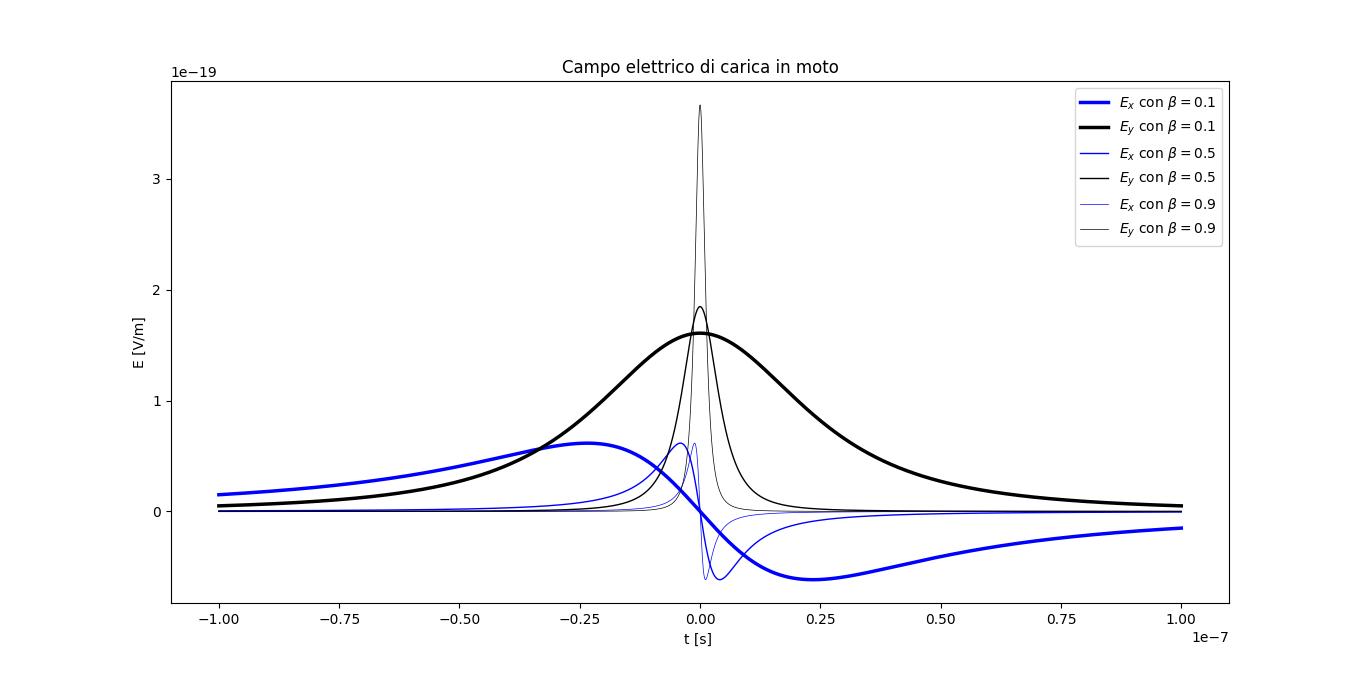
\includegraphics[width=0.8\textwidth]{immagini/carica_in_moto.png}
	\caption{Campi elettrici generati da una carica in moto}
	\label{fig:campo_carica_moto}
\end{figure}
Da notare che il campo lungo $y$ diventa sempre più stretto e piccato all'aumentare di $\beta$ (di conseguenza anche il campo magnetico, soltanto che questo è rifotto di un fattore $\beta$).

\subsection[]{Scrivere in forma covariante l'equazione del moto di una carica in un campo elettromagnetico esterno ("quadri-forza di Lorentz").}
\label{sec:3.b.7}
Analizziamo il caso di una particella puntiforme, l'equazione relativistica (tridimensionale) del moto è: \[
	\frac{\mbox{d} \bs{p}}{\mbox{d} t} = e\left( \bs{E}+ \frac{\bs{v}}{c}\wedge \bs{B} \right) 
.\] 
Nella quale l'impulso spaziale è $\bs{p}=m\gamma \bs{v}$.\\
È quindi ragionevole pensare che si debba sfruttare il 4-impulso $p^{\mu}=m u^{\mu}$ con $u^{\mu}=\gamma\left( c, \bs{v} \right)$, ed il tensore dei campi gia introdotto nelle domande precedenti, ovvero l'entità che contiene tutte le informazioni necessarie dei campi e che viene da un formalismo covariante. Per procedere si cerca quindi una equazione della forma:
\[
	\frac{\mbox{d} p^{\mu}}{\mbox{d} \tau}= N F^{\mu\nu} u_{\nu} 
.\]
Cercando una normalizzazione $N$ ragionando sulle dimensioni: per trarre una forza dall'espressione di destra ci serve una carica a moltiplicare ed una velocità a dividere, si prova ad utilizzare $\frac{e}{c}$. Si prova quindi componente per componente:
\begin{align*}
	F^{0i}u_{i}=& -E_{i}\cdot \left( -\gamma v_{i} \right) =\gamma \bs{E}\cdot \bs{v}\\
	F^{i\alpha}u_{\alpha}=&F^{i 0}u_0+F^{ij}u_{j}=E_{i}c\gamma-\epsilon_{ijk}B_{k}\left( -\gamma v_{j} \right) =\\
	=& c\gamma\left(\bs{E}+\frac{\bs{v}}{c}\wedge \bs{B}   \right) 
.\end{align*}
Considerando il fatto che 
\[
	dt= \gamma d\tau
\]
si ha che li componenti spaziali (le seconde calcolate) danno proprio l'equazione del moto.\\
Considerando invece che $P^{\mu}=\left(\varepsilon /c, \bs{p} \right)$ si ha che la componente temporale rappresenta il teorema delle forze vive:
\[
	\frac{\mbox{d} \varepsilon}{\mbox{d} t} = e \bs{E}\cdot \bs{v}	
.\] 


\subsection[]{Dimostrare che la forza di reazione radiativa è: 
\[
	\bs{F}_{\text{rad}}=\frac{2q^2}{3c^3}\dot{\bs{a}}=z^2m_e \tau_e \dot{\bs{a}} \quad \quad \text{con } \tau_e=\frac{2r_{e}}{3c}=\left(6.2\cdot 10^{-24}\right)
.\]
Indicare inoltre il campo di applicazione di quest'ultima.
}\label{sec:3.b.8}
La dimostrazione euristica e non relativistica è stata affrontata nella \hyperref[subsec: 2.a.15]{Domanda 2.a.15} insieme ai campi di applicazione (moto periodico). 

\subsection[]{Dare la definizione del "tensore energia-impulso" del campo elettromagnetico e scrivere la sua relazione con la "densità di forza di Lorentz".}
\label{sec:3.b.9}
Il tensore energia impulso è definito come:
\[
	\Theta^{\mu\nu}=\frac{1}{4\pi}\left( F^{\mu\alpha}F^{\nu}_{\alpha}- \frac{1}{4}\eta^{\mu\nu}F^{\alpha\beta}F_{\alpha\beta} \right) 
.\] 
Dove $\eta^{\mu\nu}$ è il tensore metrico diag$\left( 1,-1,-1,-1 \right)$.\\
Per inquadrarlo meglio lo si può vedere sotto forma di matrice: 
\[
	 \Theta= 
	 \left(
		 \begin{array}{c|ccc}
			 u_{\text{em}} 	& 		&	\bs{S}  	&	\\   
		 	\hline	 
					&		&  			&	\\
		 	\bs{S} 		&  		&  	-T_{\text{Maxwell}}		& 	\\
		 	 		&  		&  			& 	\\
		 \end{array}
	 \right) 
.\] 

Tale tensore è legato alla densità di forza di Lorentz da:
\[
	\partial_{\mu}\Theta^{\mu\nu}+f^{\nu}=0
.\] 
Dove la densità di forza di Lorentz ricordiamo essere: \[
	f^{\nu}=\frac{1}{c}F^{\mu\nu}j_{\nu}=\left( \frac{\bs{j}\bs{E}}{c}, \rho \bs{E}+\frac{1}{c} \bs{j}\wedge \bs{B}  \right) 
.\] \label{eq:conservazioni-relativita} 
\subsection[]{Dire come si generalizzano i teoremi di conservazione dell'energia e dell'impulso a situazioni in cui sia presente un campo elettromagnetico.}
\label{sec:3.b.10}
Nel caso dell'energia si ha (CGS):
\[
	\frac{1}{8\pi}\frac{\partial }{\partial t} \left( E^2+B^2 \right) + \frac{c}{4\pi}\nabla\left( \bs{E}\wedge \bs{B} \right) = - \bs{E}\cdot \bs{j}
.\] 
Nel caso dell'impulso invece: \[
	\frac{1}{4\pi}\frac{\partial}{\partial t}\left(\bs{E}\wedge\bs{B}\right)+\nabla\cdot T=-\left(\rho\bs{E}+\frac{\bs{j}}{c}\wedge \bs{B}\right) 
.\]
Con T tensore degli stress di Maxwell.\\
Entrambe le equazioni sono generaliate al caso relativistico dalla \hyperref[eq:conservazioni-relativita]{Equazione} che lega la densità di forza di Lorentz al tensore energia impulso.

\subsection[]{Scrivere il tensore degli sforzi per un’onda e.m. piana che si propaga in una direzione definita come $\hat{n}$.}
\label{sec:3.b.11}
Il tensore degli stress è definito come:
\[
	T= \I u_{\text{em}} - \frac{1}{4\pi} \left( E \otimes E + B \otimes B\right) 
\]
Oppure con gli indici:
\[
	T^{ij}= \delta^{ij}u_{\text{em}} - \frac{1}{4\pi}\left( E^{i}E^{j}+ B^{i}B^{j} \right) 
\]
Con 
\[
	u_{\text{em}}=\frac{1}{8\pi}\left( E^2 + B^2 \right) = \frac{1}{8\pi}\left( E_{i}E_{i}+ B_{j}B_{j} \right)
.\]
Quindi con un'onda piana che propaga nella direzione $\hat{n}$ si ha sempre (con una opportuna rotazione del sistema di riferimento) che \[
	T^{ij}=n^{i}n^{j}u_{\text{em}}
.\] 
Per verificarlo basta scegliere il sistema di riferimento in cui l'onda piana propaga nella direzione $\hat{x}=\hat{n}$, in questo modo si ha:
\begin{align*}
	\bs{E}=&E_0 \hat{y} e^{ikx-i \omega t}\\
	\bs{B}=&B_0 \hat{z} e^{ikx-i\omega t}
.\end{align*}
Da cui segue immediatamente che \[
	T^{ij}= \delta^{ij} \frac{E_{i}E_{i}+B_{i}B_{i}}{8 pi} - \frac{1}{4\pi}\left(  E^{i}E^{j}+B^{i}B^{j}\right)
\]
Non ci scordiamo che $E_i$ è diverso da zero solo con $i=1$ (ovvero per la componente $y$), allo stesso modo  $B_i$ è diverso da zero solo con $i=2$. Questo comporta che il secondo termine (quello con il segno meno nella espressione sopra) non si annulla solo per il secondo ed il terzo elemento diagonale (yy e zz) in cui vale $u_{\text{em}}$, tuttavia in entrambi i casi questi vengono annullati dalla presenza del primo termine (che è anche esso diagonale).\\
Infatti, essendoci una $\delta$, il primo termine si collocherà nella matrice $T$ solo sugli elementi diagonali, portando in ognuno di essi lo stesso scalare $u_{\text{em}}$. \\
Se ne conclude che:
\[
	T^{ij}=  u_{\text{em}}n^{i}n^{j}
.\] 
Dove il prodotto scalare tra $n^{i}$ e $n^{j}$ è solo un modo compatto per esprimere la matrice che scriveremo tra poco.
\begin{align*}
	\hat{n}=
	\left( 
	\begin{array}{c}
		i=0 \implies 1\\
		i=1 \implies 0\\
		i=2 \implies 0
	\end{array}
	\right) 
.\end{align*}
Facendo scorrere gli indici e provando a combinarli si trova la forma matriciale di $T$ :
\[
	T=
	u_{\text{em}}
	\left(
	\begin{array}{ccc}
		1 & 0 & 0 \\   
		0 & 0 & 0 \\
		0 & 0 & 0 \\
	\end{array}
	\right)
.\] 
\subsection[]{Scrivere esplicitamente il 4-tensore impulso-energia per un’onda elettromagnetica piana monocromatica che si propaga lungo l’asse x con densita’ di energia $u_{\text{em}}$.}
\label{sec:3.b.12}
Utilizzando i risultati della domanda 3.b.9 e 3.b.11 possiamo dire che:
\[
\Theta=
\left(
\begin{array}{cccc}
	u_{\text{em}} & u_{\text{em}}  & 0 & 0 \\   
	u_{\text{em}} & -u_{\text{em}} & 0 & 0 \\
	0 & 0 & 0 & 0 \\
	0 & 0 & 0 & 0 \\
\end{array}
\right)
.\] 


\subsection[]{Ricavare l’espressione per i potenziali di Lienard-Wiechert ( $\phi$ ed A per una carica puntiforme in moto arbitrario) a partire dai potenziali ritardati.}
\label{sec:3.b.13}
Ricordiamo l'espressione dei potenziali ritardati:
\begin{align*}
	\varphi\left( \bs{r},t \right)=	& \int \frac{\rho\left( \bs{r}', t-\left| \bs{r}-\bs{r}' \right|/c \right) }{\left| \bs{r}-\bs{r}' \right| }d^3r'\\
					&\\
	\bs{A}\left( \bs{r},t \right)=	& \frac{1}{c}\int \frac{\bs{j}\left( \bs{r}', t-\left| \bs{r}-\bs{r}' \right|/c \right)}{\left| \bs{r}- \bs{r}' \right|} d^3r'
.\end{align*}
Sia Q una carica che si muove con la legge oraria $\bs{s}\left( t \right) $, le densità di carica e di corrente ad essa assoiate sono:
\begin{align*}
	\rho\left( \bs{r},t \right) =&q\delta^3\left( \bs{r}-\bs{s}\left( t \right) \right)\\
	\bs{j}\left( \bs{r},t \right) =&q \dot{\bs{s}}\left( t \right) \delta^3\left(\bs{r}-\bs{s}\left( t \right)   \right)
.\end{align*}
Il tempo ritardato è definito come al solito:
\[
	c\left( t- t' \right) = \left| \bs{r}-\bs{s}\left( t \right)  \right| 
.\] 
Si procede quindi al calcolo del potenziale scalare, il calcolo del potenziale vettore è del tutto analogo.
\[	
	\varphi\left( \bs{r},t \right)=	 q\int \frac{\delta^3\left( \bs{r}'-\bs{s}\left( t-\left| \bs{r}- \bs{r}' \right|/c \right)  \right)  }{\left| \bs{r}-\bs{r}' \right| }d^3r'\\
.\] 
Si può quindi utilizzare la prorietà della delta :
\[
	\int \delta\left( f\left( x \right)  \right) dx \ \stackrel{f\left( x \right) = y}{=} \ \int\delta\left( y \right) \frac{1}{\left| f' \right| }dy= \left. \frac{1}{\left| f' \right| }\right|_{f\left( x \right) =0}
.\] 
Ricordandoci che lo stiamo applicando ad un caso vettoriale, concentriamoci sul cambio di variabile (prima uguaglianza della relazione sopra) nel nostro integrale abbiamo:
\[
	f\left( \bs{r}' \right) = \bs{r}'- \bs{s}\left( t- \frac{\left| \bs{r}-\bs{r}' \right| }{c} \right) 
.\]
Nel calcolo della derivata consideriamo direttamente il fatto che, rimanendo una $\delta$ all'interno dell'integrale dopo il cambio di variabile, l'integrale verrà calcolato nei punti in cui la $\delta$ si annulla. Nel nostro caso si annulla in $\bs{r}' = \bs{s}\left( t' \right) $, quindi calcoleremo la derivata di $f$ direttamente nel punto di annullamento della $\delta$ rimanendo astratti nella formulazione dell'integrale. 
E necessario anche notare che la parametrizzazione
\[
\hat{t}=t-\frac{\left| \bs{r}-\bs{r}' \right| }{c}
\]
è tanto valida quanto quella del tempo ritardato, deriveremo rispetto a questo tempo applicando le regole di derivazione di funzioni composte:
\begin{align*}
	\left. f'\left( \bs{r}' \right)\right|_{\bs{r}'=\bs{s\left( t' \right) }} =& \left[ 1 - \frac{\partial \bs{s}\left( t- \frac{\left| \bs{r}-\bs{r}' \right| }{c} \right) }{\partial \left( t - \frac{\left| \bs{r}-\bs{r}' \right| }{c} \right) } \cdot  
			\frac{\partial}{\partial \bs{r}'} \left( t- \frac{\left| \bs{r}-\bs{r}' \right| }{c} \right) \right]_{\bs{r}'=\bs{s}\left( t' \right) } =\\
			=&\left[ 1 - \frac{\bs{v}\left( t-\frac{\left| \bs{r}-\bs{r}' \right| }{c} \right) }{c}\cdot \frac{\left( \bs{r}-\bs{r}' \right) }{\left| \bs{r}-\bs{r}' \right| }\right]_{\bs{r}'=\bs{s}\left( t' \right) } =\\
	=& 1-\bs{\beta}\cdot \hat{n}
.\end{align*}

Inoltre è necessario scrivere il denominatore dell'integranda in funzione della nuova variabile y, senza perdere di generalità possiamo scriverlo come :
\[
	\left| \bs{r}-\bs{r}' \right| = \left| \bs{r}-f^{-1}\left( y \right)  \right| 
.\] 
Detto ciò l'integrale diventa:
\[
	\varphi\left( \bs{r}, t \right) = q\int \frac{\delta\left( y \right)}{\left| \bs{r}-f^{-1}\left( y \right)  \right| } \frac{1}{\left| f'\left( y \right)  \right| }dy 
.\]
Applicando la $\delta$ esce dall'integrale un termine $f^{-1}\left( y=0 \right) $; non è necessario esplicitarlo, basta applicare nuovamente l'operatore di inversione per farlo tornare $\bs{r}'$ calcolato in $\bs{s}\left( t' \right) $. Si conclude quindi che:
\[
	\varphi\left( \bs{r}, t \right) = \left[\frac{q}{\left| \bs{r}-\bs{s}\left( t \right)  \right| \left( 1-\bs{\beta}\left( t \right) \cdot \hat{n} \right) }\right]_{t=t'}
.\] 
Analogamente possiamo ricavare il potenziale vettore:
\[
	\bs{A}\left( \bs{r}, t \right) =\left[\frac{q \bs{\beta\left( t \right) }}{\left| \bs{r}-\bs{s}\left( t \right)  \right| \left( 1-\bs{\beta}\left( t \right) \cdot \hat{n} \right) }\right]_{t=t'}
.\] 

\subsection[]{Calcolare la potenza totale irraggiata da una carica accelerata in moto non relativistico. Esprimere i risultati in MKSA e nelle unità “naturali”.}
\label{sec:3.b.14}
Il campo elettrico di una carica in zona di radiazione è (nell'approssimazione non relativistica):
\[
	\bs{E}_{\text{rad}}\left( \bs{x},t \right)= \frac{q}{c} \left[ \frac{\hat{n}\wedge \left[ \left( \hat{n}-\bs{\beta} \right) \wedge \dot{\bs{\beta}}  \right] }
	{\left( 1-\hat{n}\cdot \bs{\beta} \right) R}  \right]_{\text{rit}}  \approx \frac{q}{c}\left[ \frac{\hat{n}\wedge \left(\hat{n}\wedge \dot{\bs{\beta}}\right)}{R}\right]_{\text{rit}} 
\]
Essendo il campo $\bs{B}=\hat{n}\wedge \bs{E}$ dal calcolo del vettore di Poynting si conclude che (conto affrontato nella domanda \hyperref[sec:3.b.3]{Domanda 3.b.3}):
\[
	\frac{\mbox{d} P}{\mbox{d} \Omega} = \frac{q^2\left| \hat{n}\wedge \dot{\bs{\beta}}\right|^2}{4\pi c}
.\] 
Integrando sull'angolo solido si ottiene che (sistema di riferimento con coordinate sferiche):
\[
	P = \frac{2q^2\left| \dot{\bs{\beta}} \right|^2}{3c}
.\] 
In MKSA si ottiene:
\[
	P = \frac{q^2\left| \dot{\bs{\beta}} \right|^2}{6\pi\epsilon_0c}
.\] 

\subsection[]{Ricavare la formula di Larmor relativistica 
\[
	P=\frac{2q^2}{3c^3}\gamma^{6}\left( \left| \bs{a} \right| ^2 - \left| \bs{a}\wedge \bs{\beta}  \right| ^2 \right) 
.\] a partire dalla formula non relativistica ed utilizzando argomenti di invarianza relativistica.}
\label{sec:3.b.15}
La potenza deve essere un invariante relativistico. Infatti è definita dal rapporto tra un energia ed un tempo, entrambe prime componenenti di un quadrivettore e quindi entrambe trasformanti allo stesso modo (come un tempo).\\
Conviene allora sfruttare l'invariante $a^{\mu}a_{\mu}$, con $a^{\mu}$ quadriaccelerazione definita da:
\[
	a^{\mu}=
	\left( \quad
	\begin{array}{c}
		\gamma^{4}\bs{a}\cdot \bs{\beta}, \quad 
		\gamma^2 \bs{a}+\gamma^{4} \left( \bs{a}\cdot \bs{\beta} \right) \bs{\beta}
	\end{array}
	\quad \right)
.\] 
Possiamo provare a vedere se la quantità giusta è: \[
	P=-\frac{2}{3} \frac{q^2}{c^3}a^{\mu}a_{\mu}
.\] 
Che è un invariante di Lorentz e soprattutto coincide con la formula non relativistica. Proviamo a vedere se torna con il caso cercato:
\begin{align*}
	a^{\mu}a_{\mu}=&\gamma^{4}\left( \gamma^{4}\left( \bs{a}\cdot \bs{\beta} \right) ^2 - \left| \bs{a}+ \gamma^2\left( \bs{a}\cdot \bs{\beta} \right) \bs{\beta} \right| ^2 \right)=\\
	=& \gamma^{4}\left( \gamma^{4}\left( \bs{a}\cdot \bs{\beta} \right)^2-\gamma^{4}\left| \bs{\beta} \right|^2 \left( \bs{a}\cdot \bs{\beta} \right)^2 - \left| \bs{a} \right| ^2 - 2\gamma^2\left( \bs{a}\cdot \bs{\beta} \right) ^2   \right) =\\
	=& \gamma^{4}\left( -\gamma^2\left( \bs{a}\cdot \bs{\beta} \right)^2-\left| \bs{a} \right|^2 \right)=\\
	=& \gamma^{6}\left( \left| \bs{\beta} \right|^2\cdot  \left| \bs{a} \right|^2 - \left( \bs{a}\cdot \bs{\beta} \right)^2 - \left| \bs{a} \right|^2\right)=\\
	=& \gamma^{6}\left( \left| \bs{a}\wedge \bs{\beta}  \right|^2-\left| \bs{a} \right|^2 \right) 
.\end{align*}
Da cui se ne conclude che la quantità provata è quella giusta.

\subsection[]{Dimostrare che la radiazione di sincrotrone ha uno spettro di emissione con una frequenza “critica” $\omega_{u}\approx \omega_0\gamma^3$.}
\label{sec:3.b.16}
Per arrivare al risultato costruiamo geometricamente la situazione di osservazione:
\begin{figure}[ht]
    \centering
    \incfig{luce-sincrotrone}
    \caption{Schema di rilevamento della Luce di Sincrotrone}
    \label{fig:luce-sincrotrone}
\end{figure}
Alla posizione $R$ di Figura c'è un rilevatore di radiazione elettromagnetica, la circonferenza rappresentata è la traiettoria della particella nell'acceleratore. Si rappresentano gli istanti $t'_{1}$ e $t'_{2}$ in cui la radiazione (che può essere rilevata da $R$) viene emessa dalla sorgente. Se la radiazione emessa in tali istanti viene rilevata allora arriva al rivelatore rispettivamente agli istanti $t_{1}$ e $t_{2}$, questa notazione induce le relazioni:
\begin{align*}
	t_1 =& t'_{1}+ \frac{\Delta L + D}{c}\\
	t_2=& t'_{2}+ \frac{D}{c}=t'_{1}+ \frac{\Delta L}{V}+ \frac{D}{c}
.\end{align*}
Possiamo allora dare una stima del tempo in cui si osserva la radiazione come:
\begin{align*}
	\Delta t =& t_2-t_1 =\\
	=&\frac{\Delta L}{V}- \frac{\Delta L}{c}=\\
	=& \Delta L \left( \frac{1}{\beta c} - \frac{1}{c} \right) 
.\end{align*}
Adesso dobbiamo sfruttare il fatto che per particelle che viaggiano a velocità relativistiche $1 /\gamma \approx 1$, quindi l'angolo in figura taglierà un arco di circonferenza piccolo rispetto alle dimensioni dell'apparato. Quindi:
\begin{align*}
	\Delta L \approx \frac{2 \rho}{\gamma} \quad \implies \quad  \Delta t \approx \frac{2\rho}{\gamma}\left( \frac{1-\beta}{\beta c} \right) 
.\end{align*}
Infine moltiplicando e dividendo per $1+\beta$:
\[
	\Delta t = \frac{2 \rho}{\gamma \beta c} \left( \frac{1-\beta^2}{1+\beta} \right)\approx \frac{\rho}{c \gamma^3} 
.\] 
Logicamente se l'impulso dura $\Delta t$ significa che lo spettro angolare di radiazione si estende fino ad una frequenza critica:
\[
	\omega_{c} \sim \frac{1}{\Delta t} = \frac{c\gamma^3}{\rho}= \omega_0\gamma^3
.\] 

\subsection[]{Calcolare il fattore di forma elettromagnetico per una sfera uniformente carica di raggio a.}
\label{sec:3.b.17}
La sfera di raggio $a$ uniformemente carica avrà una distribusione di carica esprimibile come:
\begin{align*}
	\rho\left( \bs{r} \right) =
	\begin{cases}
	\ \frac{3Q}{4\pi a^3} \quad &\text{se} \quad \left| \bs{r} \right| < a  \\
	\ 0  \quad  &\text{se} \quad \left| \bs{r} \right| > a \\
	\end{cases} 
.\end{align*}
Per un dato valore di $q$ scegliamo delle coordinate polari aventi l'asse polare diretto lungo $q$ stesso, si calcola quindi il fattore di forma come:
\begin{align*}
	F\left( \bs{q} \right) 	&= \frac{\int \rho\left( \bs{r} \right) e^{-i \bs{q}\cdot \bs{r}}d^3r}{\int \rho\left( \bs{r} \right) d^3r} \\
			       	&= \frac{1}{Q}\int_{0}^{a}dr\int_{0}^{\pi}d\theta \int_{0}^{2\pi} d\phi \rho\left( r \right) e^{-irq\cos\theta} r^2 \sin\theta \\
			     	&=  \frac{2\pi}{Q}\int_0^a\int_{1}^{-1} \rho\left( r \right) e^{-irq\cos\theta} r^2 \left| d\cos\theta \right| dr=\\ 
				&= \frac{4\pi}{Q} \int_0^{a} \rho\left( r \right) r^2 \frac{\sin\left( qr \right) }{qr}dr= \\
				&= \frac{3}{a^3q}\int_0^{a} r \sin\left( qr \right) dr= \\
				&= \frac{3}{a^3} \left(- \frac{1}{q} r\cos\left( qr \right) + \frac{1}{q^2} \sin \left( qr \right)  \right)_{0}^{a}= \\
				&= 3\left( \frac{\sin\left( aq \right) }{\left( aq \right)^3 } -\frac{\cos\left( aq \right) }{\left( aq \right) ^2} \right)  
.\end{align*}
In quest'ultima si può notare che, grazie alla simmetria del sistema sotto rotazioni, $F\left( \bs{q} \right) = F\left( q \right) $
\subsection[]{Calcolare il fattore di forma per una supeficie sferica uniformente carica di raggio a. [nota: l'interno è vuoto]}
\label{sec:3.b.18}
In tal caso la densità di carica si può esprimere come:
\begin{align*}
	\rho\left( \bs{r} \right) =
	\begin{cases}
		\ 0 \quad \text{se} \quad  \left| \bs{r} \right| < a\\
		\ \frac{Q}{ 4 \pi a^2} \quad \text{se} \quad \left| \bs{r} \right| = a\\
		\ 0 \quad \text{se} \quad \left| \bs{r} \right| > a
	\end{cases}
.\end{align*}
Procedendo come sopra senza interare su $r$ si ottiene:
\[
	F\left( \bs{q} \right) = \frac{3\sin\left( aq \right) }{a^2q}
.\] 

\subsection[]{Calcolare la velocità di un elettrone [e successivamente di un protone] posto in una struttura acceleratrice che abbia: \\
	1) Campo elettrico longitudinale costante.\\ 
	2) Campo elettrico longitudinale oscillante.\\ 
Inserendo valori numerici ragionevoli, calcolare il tempo affinché la particella, partendo da ferma, raggiunga una energia pari al doppio della sua massa a riposo.}
\label{sec:3.b.19}
Supponiamo la struttura lineare, l'equazione di moto di una particella nel campo dell'acceleratore è:
\[
	\frac{\mbox{d} }{\mbox{d} t} \left( p_{x} \right) = qE \implies	\frac{\mbox{d} }{\mbox{d} t}\left( \gamma \beta \right)  = \frac{qE}{mc}
.\] 
\paragraph{Campo elettrico costante}%

Nel caso di campo costante l'equazione si risolve con:
\[
	\gamma \beta = \frac{qE}{mc}\cdot  t = \frac{t}{\tau}
.\] 
Per trovare la velocità (quindi $\beta$) dobbiamo esplicitare $\gamma$ nella precedente:
\[
	\frac{\beta^2}{1-\beta^2}= \frac{t^2}{\tau^2}\implies \beta=\frac{t}{\sqrt{t^2+\tau^2} }
.\] 
Da cui l'energia:
\[
	E= mc^2\gamma= mc^2\sqrt{1+\frac{t^2}{\tau^2}} 
.\] 
Ne segue che per avere una energia che sia il doppio di quella a riposo bisogna imporre:
\begin{align*}
	2=\sqrt{1+\frac{\Delta t^2}{\tau^2}} \implies \Delta t = \sqrt{3}\tau \approx 
	\begin{cases}
		10^{-11} & \text{per l'elettrone}\\
		10^{-7} &  \text{per il protone}
	\end{cases} 
.\end{align*}
Nella stima numerica è stato preso il valore tipico di campo elettrico per un acceleratore lineare di $50$ MeV/m.
\paragraph{Campo elettrico oscillante}%
Gli acceleratori costruiti con questo metodo accelerano le particelle solo nel semiperiodo in cui il campo elettrico è diretto nella direzione in cui è attesa la accelerazione, per far ciò si alternano zone in cui il campo è presente a zone in cui invece non lo è.
\begin{figure}[H]
	\centering
	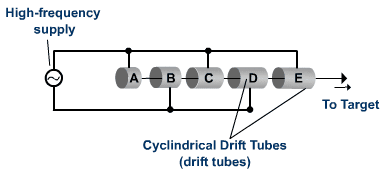
\includegraphics[width=0.4\textwidth]{immagini/drift-tube.png}
	\caption{Drift Tube in un acceleratore lineare}
	\label{fig:Drift Tube}
\end{figure}
Prendiamo adesso un campo elettrico del tipo :
\[
	E= E_0\sin\left( \frac{\pi t}{\tau'} \right) 
.\] 
Non possiamo più applicare il metodo utilizzato sopra, potremmo in qualche modo cercare di discretizzare il problema mediando l'equazione del moto su un semiperiodo (per i motivi spiegati all'inizio), la variabile diventa allora il tempo impiegato a fare un semiperiodo $\tau'$:
\[
	\Delta \left( \beta\gamma \right) = \frac{qE_0}{mc}\int_0^{\tau'} \sin \left( \frac{\pi t}{\tau} \right) dt = \frac{2qE_0\tau'}{\pi mc}
.\] 
Quindi ogni volta che la particella attraversa un Drift tube subisce una variazione di $\gamma\beta$ come quella scritta sopra.
Se parametrizziamo il modulo del campo elettrico iniziale come:
\[
	E_0 \rightarrow \frac{2E_0}{\pi} = E'_0
.\] 
ci si accorge che il risultato non è tanto differente da quello incontrato nel caso di campo costante (ipotizziamo sempre che la particella sia idealmente ferma nel momento dell'accenzione del campo).
\[
	\Delta \gamma\beta = \gamma_{\text{fin}}\beta_{\text{fin}}=\frac{qE'_0}{mc}\tau'=\frac{\tau'}{\hat{\tau}}
.\] 
con $\hat{\tau}=\frac{qE'_0}{mc}$.\\
Notiamo che se vogliamo la quantità $\gamma\beta$ dopo che la particella ha attraversato $n$ Drift Tube basta sommare $n$ volte la quantità $\tau' /\hat{\tau}$.
calcoliamo la velocità della particella all'uscita dell'ennesimo Drift Tube sfruttando il calcolo effettuato in precedenza:
\[
	\beta = \frac{n \tau'}{\sqrt{\hat{\tau}^2 + n^2 \tau'^2} }
.\] 
E in modo analogo l'energia:
\[
	E = mc^2\sqrt{1+\frac{n^2\tau'^2}{\hat{\tau}^2}} 
.\] 
La ricerca del tempo in cui la particella raggiunge il doppio dell'energia a riposo richiede questa volta una piccola considerazione aggiuntiva: per ogni semi periodo trascorso in presenza del campo elettrico ve ne è uno trascorso all'esterno dei Drift Tube. Dobbiamo quindi aggiungere al tempo necessario all'interno dei drift tube (sempre in termini di semi periodi) il tempo trascorso all'esterno senza campo elettrico ed a velocità costante.
\[
	n\tau' + n\tau' = \sqrt{3}\hat{\tau} \implies 2n\tau' = \sqrt{3} \hat{\tau}
.\] 
E chiamando $2\tau'= T$ il periodo di oscillazione si ha:
\[
	nT = \sqrt{3}\frac{2qE_0}{\pi mc}
.\] 
I tempi in cui si riesce a raddoppiare l'energia hanno la stessa espressione  (fattore $\frac{2}{\pi}$ a parte), visto che le tensioni che si riesce a raggiungere nei due casi sono simili anche il valore numerico di tali tempi non differisce di molto.

\subsection[]{A partire dai campi ritardati, dimostrare che 
\[
	\frac{\mbox{d} P}{\mbox{d} \Omega} = \frac{q^2\left| \bs{a} \right|^2\sin^2\theta }{16\pi^2\epsilon_0c^3\left( 1-\beta\cos\theta \right)^5 }
.\] è la potenza (MKSA) irraggiata da una carica accelerata in un moto rettilineo.}
\label{sec:3.b.20}
I campi ritardati citati nel testo sono:
\[
	\bs{E}\left( \bs{x},t \right)= \frac{q}{c} \left[ \frac{\hat{n}\wedge \left[ \left( \hat{n}-\bs{\beta} \right) \wedge \dot{\bs{\beta}}  \right] }
	{\left( 1-\hat{n}\cdot \bs{\beta} \right)^3 R}  \right]_{\text{rit}} 
.\] 
Nel caso affrontato essendo il moto rettilineo velocità ed accelerazione sono parallele, quindi:
\[
	\bs{E}\left( \bs{x},t \right)= \frac{q}{c} \left[ \frac{\hat{n}\wedge \left( \hat{n}  \wedge \dot{\bs{\beta}}  \right) }
	{\left( 1-\hat{n}\cdot \bs{\beta} \right)^3 R}  \right]_{\text{rit}} 
.\] 
Come sempre si può ricavare il vettore di Poynting utilizzando il modulo quadro del campo elettrico:
\[
	\bs{S\left( t \right) }= \frac{c}{4 \pi }\left| \bs{E} \right|^2_{\text{rit}} \hat{n} = 
	\frac{q^2}{4 \pi c}\left|  \frac{\hat{n}\wedge \left( \hat{n}  \wedge \dot{\bs{\beta}}  \right) }{\left( 1-\hat{n}\cdot \bs{\beta} \right)^3 R^2} \right|^2_{\text{rit}} \hat{n}
.\] 
In questo modo si ha il vettore di Poynting parametrizzato per unità di tempo, infatti con questo potremmo calcolare l'energia che attraversa l'elemento infinitesimo di area come:
\[
	W= \int_{-\infty}^{\infty} dt \bs{S}\left( t \right) \cdot \hat{n}
.\] 
Se nell'integrale facciamo il cambio di variabile
\[
	W= \int_{-\infty}^{\infty} dt' \frac{dt}{dt'} \bs{S}\left( t\left( t' \right)  \right) \cdot \hat{n}
.\]
Possiamo ridefinire l'integranda come la potenza irraggiata istantaneamente dalla particella
\[
	\frac{\mbox{d} W}{\mbox{d} t'}= \frac{dt}{dt'} \bs{S}\left( t\left( t' \right)  \right) \cdot \hat{n} 
.\] 
calcolata al tempo in cui la radiazione viene emessa e non al tempo ritardato, ovvero esattamente quella che vogliamo considerare. 
Lo Jacobiano di questo cambio di variabile è (calcolato nella \hyperref[sec:3.b.1]{Domanda 3.b.1}):
\[
	\frac{dt}{dt_{\text{rit}}}= 1- \hat{n}\cdot \bs{\beta}
.\] 
Quindi la potenza irraggiata per unità di angolo solido tornando in MKSA è (come già visto nella \hyperref[sec:3.b.3]{Domanda 3.b.3}): 
\begin{align*}
	\frac{\mbox{d} P}{\mbox{d} \Omega} &= \left| \bs{S} \right| R^2 =\\
	&=  \frac{q^2}{16\pi^2\epsilon_0 c} \left|  \frac{\hat{n}\wedge \left( \hat{n}  \wedge \dot{\bs{\beta}}  \right) }{\left( 1-\hat{n}\cdot \bs{\beta} \right)^3 } \right|^2\left( 1-\hat{n}\cdot \bs{\beta} \right) =\\
	&=  \frac{q^2}{16\pi^2\epsilon_0 c} \frac{\left| \hat{n}\wedge \left( \hat{n}\wedge \dot{\bs{\beta}}  \right)   \right|^2 }{\left( 1-\hat{n}\cdot \bs{\beta} \right)^{5} }
.\end{align*}
Per concludere la dimostrazione manca adesso il sistema di riferimento in coordinate sferiche, facendo riferimento alla seguente figura
\begin{figure}[H]
    \centering
    \incfig{sistema-potenza-relativistica}
    \caption{Sistema di riferimento per una carica accelerata linearmente.}
    \label{fig:sistema-potenza-relativistica}
\end{figure}
è facile concludere l'uguaglianza tra la formula trovata in forma vettoriale sopra e quella richesta nel testo.



\subsection[]{Calcolare l’energia persa in una rivoluzione per una carica in moto uniforme su una circonferenza (acceleratore circolare). Calcolare la frazione di energia persa
in un giro rispetto alla sua energia cinetica, effettuando una valutazione numerica, nel caso di elettroni a LEP (energia 50 GeV, raggio 4km) o protoni ad LHC (energia 7 TeV, raggio ~4km). Nota: utilizzare la formula di Larmor in GCS:
\[
	P=\frac{2q^2}{3c^3}\gamma^{6}\left( \left| \bs{a} \right| ^2 - \left| \bs{a}\wedge \bs{\beta}  \right| ^2 \right) 
.\] }
\label{sec:3.b.21}
Sia $a$ l'accelerazione radiale della particella nel suo moto, $R$ il raggio di curvatura totale e $R_{B}$ il raggio di curvatura nel tratto esclusivamemnte composto da zone con campo magnetico (quelle adibite a curvare).\\
Nel caso di moto uniforme su una circonferenza abbiamo visto nella \hyperref[sec:3.a.21]{Domanda 3.a.21} che la formula di Larmor si può riscrivere come (CGS):
\[
	P = \frac{2\gamma^4\beta^4}{3}\frac{q^2c}{R_{B}^2}
.\] 
O anche, per effettuare stime numeriche, in MKSA:
\[
	P = \frac{\gamma^4\beta^4}{6\pi\epsilon_0}\frac{q^2c}{R_{B}^2}
.\] 
Per una stima della energia persa al giro in irraggiamento dobbiamo considerare solo le zone in cui vi è accelerazione di carica, quindi le zone di curvatura in cui vi è un campo magnetico. Tale tempo, se la particella viaggia a velocità costante è:
\[
	T_{B}= \frac{2\pi R_{B}}{\beta c}
.\] 
Quindi la variazione di energia sul giro (aggiungiamo e togliamo termini per renderla più interpretabile):
\begin{align*}
	\Delta E &= P\cdot T_{B}=\\
	&=  \frac{\gamma^4\beta^4}{6\pi\epsilon_0}\frac{q^2c}{R_{B}^2}\frac{2\pi R_{B}}{\beta c}=\\
	&=  \frac{4\pi }{3}\frac{q^2}{4\pi\epsilon_0m_e c^2} m_ec^2\frac{\beta^3\gamma^4}{R_B}\\
	&= \frac{4\pi}{3}\left( \frac{r_e}{R_B} \right) m_e c^2\beta^3\gamma^4 \\
\end{align*}	
Possiamo quindi già fare una prima stima numerica lasciando liberi i parametri che variano nei due casi:
\[
\Delta E \approx 4 \cdot 2.8 \text{ [fm]}\cdot 0.51 \text{ [MeV]} \frac{\beta^3\gamma^4}{R_B} \approx 5.6 \text{ [fm]} \cdot \text{[MeV]} \frac{\beta^3\gamma^4}{R_B} 
.\] 
Con i dati del testo possiamo calcolare le quantità necessarie alla stima di $\gamma$ e $\beta$:
\begin{align*}
	&\gamma = \frac{E}{mc^2}  &\beta = \sqrt{1- \frac{1}{\gamma^2}} 
.\end{align*}

\paragraph{Acceleratore LEP}%
In tal caso si ha $\gamma=(50 \cdot 10^{3}) / 0.51 \approx 10^5$, $\beta \approx 1$ quindi:
\begin{align*}
	& \Delta E \approx \frac{5.6 \cdot 10^{-15}}{4 \cdot 10^{3}} \cdot 10^{20}\text{ [MeV]}=1.4 \cdot 10^{2} \frac{\text{ [MeV]} }{\text{giro}} = 
	0.14 \frac{\text{ [GeV]} }{\text{giro}}
.\end{align*}
Che da quindi una frazione di energia persa per giro di $\Delta E / E \approx 0.3 \%$
\paragraph{Acceleratore LHC}%
La massa del protone fa la differenza su $\gamma$ e su $\beta$ :
\begin{align*}
	&\gamma = \frac{7 \cdot 10^{6} \text{ [MeV]}}{9.383 \cdot 10^{2}  \text{ [MeV]}}\approx 7.5 \cdot 10^{3} \\
	&\beta \approx \sqrt{1- 10^{-8}}\approx 1 
.\end{align*}
Per l'energia quindi:
\begin{align*}
	& \Delta E \approx \frac{5.6 \cdot 10^{-15} }{4 \cdot 10^{3} } \left( 7.5 \cdot 10^{3}  \right) ^4 \text{ [MeV]} \sim \text{ [eV]}  
.\end{align*}
Da cui si deduce che la frazione di energia persa per irraggiamento nel caso di protoni è pressochè nulla.

\subsection[]{Calcolare la potenza emessa in funzione dell’angolo per una carica oscillante armonicamente in linea retta (termine di dipolo elettrico)}
\label{sec:3.b.22}
Potremmo riallacciarci al campo di radiazione del dipolo sempre passando per i campi di radiazione di Lineard-Wiechert nell'approssimazione non relativistica:
\begin{align*}
\bs{E}_{\text{rad}}\left(\bs{x},t\right) 	&\approx\frac{q}{c}\left[\frac{\hat{n}\wedge\left(\hat{n}\wedge\dot{\bs{\beta}}\right)}{R}\right]_{\text{rit}} \\
						&= \frac{q}{c^2R} \left[ \left( \ddot{\bs{x}}\wedge \hat{n} \right)\wedge \hat{n}\right]_{\text{rit}}  \\
						&= \frac{1}{c^2R} \left( \left[ \ddot{\bs{p}} \right]_{\text{rit}}\wedge \hat{n}\right)\wedge \hat{n}
.\end{align*}
Dove $\bs{p}$ è il momento di dipolo oscillante del tipo: $\bs{p} = qx_0e^{i \omega t}\hat{x}$, preso in questo caso (a titolo di esempio) nella direzione $\hat{x}$.\\
Abbiamo visto in precedenza (\hyperref[sec:3.b.3]{Domanda 3.b.3}) che la potenza irraggiata per unità di angolo solido si può esprimere come:
\[
	\frac{\mbox{d} P}{\mbox{d} \Omega}  = R^2\left| \bs{S} \right| = R^2 \frac{c}{4\pi} \left| \bs{E}_{\text{rad}} \right|^2 
.\] 
Chiamando quindi $\theta$ l'angolo tra la direzione di oscillazione $\hat{x}$ e la direzione di osservazione $\hat{n}$ possiamo eesprimere i prodotti vettoriali in funzione di tale angolo, inoltre la doppia derivata fa scendere un fattore $\omega^2$, se ne conclude che: 
\[
	\frac{\mbox{d} P}{\mbox{d} \Omega} = \frac{\left| \bs{p} \right|^2 \omega^4}{4\pi c^3} \sin^2\theta
.\] 

\subsection[]{Calcolare, a partire dalla formula di Larmor relativistica, la potenza totale dissipata in un acceleratore lineare in funzione di $\frac{\mbox{d} \bs{p}}{\mbox{d} t}$ oppure di $\frac{\mbox{d} E}{\mbox{d} x}$ (energia fornita per unita’ di lunghezza). Dimostrare che la frazione di energia persa nell’accelerazione e’ trascurabile, fornendo adeguati valori numerici nel caso di accelerazione di elettroni o protoni.}
\label{sec:3.b.23}
Come visto nella \hyperref[sec:3.a.21]{Domanda 3.a.21} la potenza dissipata per irraggiamento in un acceleratore lineare è:
\[
	P = \frac{q^2\gamma^6}{6\pi\epsilon_0}\left| \bs{a} \right|^2=\frac{q^2}{6\pi\epsilon_0m^2}\left| \frac{\mbox{d} \bs{p}}{\mbox{d} t}  \right|^2
.\] 
Infatti per la componente spaziale del quadrimpulso si ha:
\begin{align*}
	\frac{\mbox{d} p}{\mbox{d} t} 	&= \frac{\mbox{d} mv\gamma}{\mbox{d} t} =\\
				      	&= m a \gamma + m v \frac{\mbox{d} \gamma}{\mbox{d} t} =\\
					&= ma\gamma + ma\beta^2\gamma^3=\\
					&= ma\gamma^3 
.\end{align*}
Inoltre siamo andati subito in una dimensione essendo il moto unidimensionale.
Se la volessimo in funzione della variazione lineare di energia potremmo sfruttare la relazione:
\begin{align*}
	c \frac{\mbox{d} p}{\mbox{d} t} &= \frac{\mbox{d} }{\mbox{d} t}\sqrt{E^2-m^2c^4} =\\
	&= \frac{2E}{2\sqrt{E^2-m^2c^4} }\frac{\mbox{d} E}{\mbox{d} t}=  \\
	&= \frac{E}{cp}\frac{\mbox{d} E}{\mbox{d} t} = \\
	&= \frac{mc^2\gamma}{mv\gamma c}\frac{\mbox{d} E}{\mbox{d} t} = \\
	&= \frac{1}{\beta}\frac{\mbox{d} E}{\mbox{d} t} = \\
	&= c \frac{\mbox{d} E}{\mbox{d} x}  
.\end{align*}
Quindi si otterrebbe il medesimo risultato.\\
L'uguaglianza tra le due variazioni ci è utile invece per calcolare $f_{\text{rad}}$: la frazione di energia persa rispetto all'incremento di energia:
\begin{align*}
	f_{\text{rad}}	&= \frac{P}{\frac{\mbox{d} E}{\mbox{d} t} }=\\
		      	&= \frac{q^2}{6\pi\epsilon_0 c^3m^2}\left( \frac{\mbox{d} p}{\mbox{d} t} \right)^2 \frac{1}{v \frac{\mbox{d} E}{\mbox{d} x} }=  \\
			&= \frac{2}{3\beta} \frac{r_e \left( \frac{\mbox{d} E}{\mbox{d} x}  \right) }{mc^2} 
.\end{align*}
Si vede che questa è trascurabile sempre, infatti in una distanza dell'ordine dei fm non si riescono ad ottenere variazioni di energia dell'ordine di  $mc^2$.\\
La domanda del testo era invece la frazione di energia persa $\hat{f}$, la calcoliamo sempre a partire dalla formula di Larmor:
\[
	P= \frac{q^2}{6\epsilon_0c^3}\gamma^6 a^2= 
	 \frac{q^2}{6\pi\epsilon_0c^3}\frac{1}{m^2}\left( \frac{\mbox{d} p}{\mbox{d} t}  \right)^2 
\]
sia $E_0$ il modulo del campo elettrico applicato,  si ha sempre dall'equazione di moto:
\[
	\frac{\mbox{d} p}{\mbox{d} t} = qE_0
.\] 
Introducendo questa nella potenza irraggiata:
\[
	P= \frac{q^4E^2_0}{6\pi\epsilon_0m^2c^3}
.\] 
Il calcolo da effettuare per ottenere $\hat{f}$ è:
\[
	\hat{f}= \frac{P\cdot t_f}{E_f}
.\] 
Dove $t_f$ è il tempo necessario a raggiungere l'energia finale $E_f$. Si risolve se $t_f$ è lineare in $E_f $, calcoliamo questo tempo seguendo la linea di quanto fatto nella \hyperref[sec:3.b.19]{Domanda 3.b.19}:
\[
	\gamma_f=\sqrt{1+\left( \frac{t_f}{\tau} \right)^2 } \implies t_f =
	\tau\sqrt{\gamma^2_f-1} \approx \tau \cdot \gamma_f = \frac{mc}{qE_0}\cdot \frac{E_f}{mc^2}= \frac{E_f}{qE_0 c}
.\] 
Otteniamo quindi che:
\[
	\hat{f} = \frac{q^4}{6\pi \epsilon_0m^2c^2}\frac{E_0}{q}=\frac{E_0}{E_{\text{crit}}}
.\] 
Concentriamoci su $E_{\text{crit}}$, nel caso di elettroni:
\[
	E_{\text{crit}}=q \frac{6\pi\epsilon_0m^2c^4}{q^4}= \frac{3}{2}\frac{q}{4\pi\epsilon_0 r_e^2} \approx 2.7 \cdot 10^{20} \ \frac{\text{[V]}}{\text{[m]}}
.\] 
Quindi non c'è speranza, si raggiungono al massimo i MV/m: trascurabile.\\
Nel caso di protoni invece non occorre nemmeno fare il conto: basta guardare l'espressione di $\hat{f}$, dipende inversamente dalla massa, se è trascurabile per gli elettroni lo è anche per i protoni.


\subsection[]{Calcolare la lunghezza d’onda critica della radiazione di sincrotrone (elettroni) nei casi seguenti: \\
i) energia=50GeV, raggio=4km; \\
ii) energia=5GeV, raggio=30m}
\label{sec:3.b.24}
La frequenza critica è stata calcolata nella \hyperref[sec:3.b.16]{Domanda 3.b.16}, la lunghezza d'onda critica che ne deriva è:
\[
	\lambda_c = \frac{2\pi c}{\omega_c} = \frac{2\pi\rho}{\gamma^3} 
.\] 
con $\rho$ raggio dell'acceleratore.
\paragraph{Caso i)}    $\gamma\approx 10^5 \implies \lambda_{c}\approx 2500 \text{ A}^o$
\paragraph{Caso ii)}	$\gamma\approx 10^4 \implies \lambda_{c}\approx 1.8 \text{ A}^o $


\subsection[]{Enunciare il teorema ottico e spiegarne il significato fisico nel caso di radiazione elettromagnetica su un ostacolo opaco.}
\label{sec:3.b.25}
Si consideri un'onda elettromagnetica $\bs{E}_{in}= \bs{E}_{0}e^{-i\left( \omega t - kz \right) }$ incidente su un bersaglio opaco ortogonalmente. Tale "interazione" produce una onda sferica rifratta che può essere scritta come:
\[
	\bs{E}_s= \frac{e^{-i\left( \omega t - kr \right) }}{r}\bs{f}\left( \bs{k} \right) 
.\] 
Dove $\bs{f}\left( \bs{k} \right) $ è l'ampiezza di scattering: racchiude tutta la dinamica del processo diffrattivo.\\
Si ha che la potenza dissipata in tutto il processo di scattering è:
\[
	P_{\text{diss}}= \frac{c}{2k} \text{Im}\left[ \bs{E}^*_{0}\cdot \bs{f}\left( k \hat{z} \right)   \right] 
.\] 
Che è l'enunciato del teorema ottico.

\subsection[]{Come si ricava la sezione d'urto differenziale Rayleigh a partire dalla sezione d'urto Thomson ?}
\label{sec:3.b.26}
Nello scattering Thompson si ha che, per un fotone che incide su un elettrone:
\[
	\left.\frac{\mbox{d} \sigma_{\text{el}}}{\mbox{d} \Omega}\right|_{\text{el}} =  \frac{r_e\omega^4}{\left( \omega^2_0-\omega^2 \right)^2 + \omega^2\Gamma^2_{\text{tot}}\left( \omega \right)} \sin^2\alpha
.\] 
Con $\alpha$ angolo tra la direzione di polarizzazione del campo e direzione di osservazione. Per il resto della notazione facciamo riferimento alle domande \hyperref[subsec: 2.a.15]{2.a.15} e \hyperref[subsec: 2.a.16]{2.a.16}. \\
Lo scattering Rayleigh serve invece nel caso di più centri scatteranti, come ad esempio un'onda incidente su un atomo, in tal caso è necessario introdurre nel calcolo della potenza irraggiata l'effetto della possibile interferenza tra i campi generati dai vari elettroni.\\
A questo scopo nasce il fattore di forma, tiene di conto di tali interferenze, in modo tale che se avessimo una distribuzione $\rho$ di carica con $\int \rho\left( \bs{r}\right)d^3r=Q$ il campo generato da questa non sarebbe altro che il campo di una carica puntiforme Q moltiplicato per $F\left( \bs{q} \right) $ della distribuzione.\\
Risulta quindi chiaro che l'unica correzione da aggiungere allo scattering dell'elettrone singolo è proprio il modulo quadro di questo fattore moltiplicato per il numero di elettroni presenti nell'atomo: lo scattering Rayleigh risulta:
\[
	\frac{\mbox{d} \sigma_{\text{el}}}{\mbox{d} \Omega} = \left.\frac{\mbox{d} \sigma_{\text{el}}}{\mbox{d} \Omega}  \right|_{\text{el}}\left| ZF\left( \bs{q} \right)  \right| ^2
.\] 




 % da aggiustare e fare



\section{Interazione radiazione-materia}
\setcounter{section}{0}
\renewcommand*{\theHsection}{chX.\the\value{section}}


\section{Domande a scelta}
 
\end{document}
